% !Mode:: "TeX:UTF-8"
% !TEX builder = LATEXMK
% !TEX program = xelatex
\documentclass[master,oneside]{zjuthesis} % 如果你的论文不满80页,还是单面印刷吧
% \usepackage{subfigure}
\usepackage{multirow}
%%%%%%%%%%%%%%%%%%%%%%%%%%%%%% 开始填写前置部分使用的变量
%%%%%%%%%%%%%%%%%%%%%%%%%%%%%% 样式设定在 zjuthesis.cls 下, 人类可读,爱请查阅
% \usepackage{graphicx}
\usepackage{makecell}
\usepackage{enumerate}
\usepackage{diagbox}
\usepackage{tabularx}
\usepackage{graphics}
\usepackage{booktabs}
\usepackage{amssymb}
\usepackage{amsmath}
\usepackage{makecell}

\usepackage{listings}
\usepackage{subcaption}
\usepackage{algorithmic}
\usepackage{url}
\usepackage{notoccite}
\usepackage{graphicx}
\usepackage{float}
\usepackage{chngcntr}
\usepackage[table,xcdraw]{xcolor}
\newcolumntype{Z}{>{\centering\let\newline\\\arraybackslash\hspace{0pt}}X}

% 这里写这么鬼畜是为了测试多几个字会不会造成溢出
\title{结合强化学习的图结构大语言模型关键技术研究} % 封面和题名页使用
\englishtitle{Key Techniques for Graph-Structured Large Language Models with Reinforcement Learning} % 封面和题名页使用
% 如果您的标题用字过多,请自行调节 zjuthesis.cls 里的 ZJUmakecover 里的各项距离。

%\author{}          % 申请人姓名 封面使用
\author{马晓峰}           %董爱祁

\classification{TP311.5}    % 封面头使用
\serialnumber{10335}        % 封面头使用
\secretlevel{无}            % 封面头使用
\studentnumber{22351147}    % 封面头使用

%\supervisor{御坂美琴}       % 导师 封面使用
\supervisor{耿卫东}               % {耿卫东}
%\spvtitle{电击使}           % 职称 封面使用
% \spvtitle{教授}              % 职称 封面使用{教授}
\spvtitle{教授}     
%\cpsupervisor{桂和纱}       % 合作导师,如果没有合作导师,就在此文件第 4 行\documentclass选项栏中加上"nocpsupervisor"。
\cpsupervisor{}
\cspvtitle{}             % 合作导师职称

% 从机械工程学院改来,保留设定变量命名
%\major{船舶工程}            % 专业学位类别栏 填 工程硕士
\major{电子信息}
%\research{白学}             % 专业学位领域栏 填 软件工程
\research{软件工程}
\institute{软件学院}         % 所在学位栏 填 软件学院

\submitdate{2026年3月30日}   % 论文提交日期 栏 0306

% 题名页的评阅人及答辩席
% 归档时候填写
% 论文评阅人1 2 3 4 5
\reviewerA{隐名评阅} \enreviewerA{}
\reviewerB{隐名评阅} \enreviewerB{}
\reviewerC{隐名评阅} \enreviewerC{}
\reviewerD{} \enreviewerD{}
\reviewerE{} \enreviewerE{}

% 答辩委员会主席
% \chairperson{张微$\setminus$教授级高工$\setminus$浙江大学软件学院\quad\quad\quad\quad\quad} \enchairperson{}
\chairperson{倪超$\setminus$副教授$\setminus$浙江大学软件学院} \enchairperson{}

% 答辩委员 1 2 3 4 5
\commissionerA{曾丽敏$\setminus$副教授$\setminus$浙江大学软件学院} \encommissionerA{}
\commissionerB{张文$\setminus$副教授$\setminus$浙江大学软件学院} \encommissionerB{}
\commissionerC{房子荃$\setminus$助理研究员$\setminus$浙江大学软件学院} \encommissionerC{}
\commissionerD{周鑫崴$\setminus$高级工程师$\setminus$宁波市地方金融监管局} \encommissionerD{}
\commissionerE{} \encommissionerE{}

% 答辩日期
% \defencedate{2023年3月5日} \eendefencedate{}  % 因为endefencedate 命名被占用
\defencedate{2026年3月1日} \eendefencedate{}  % 因为endefencedate 命名被占用

% 论文前置部分变量填写完毕 开始全书排版
\begin{document}
% \include{m_contents/review}      % 论文修改说明
% 封面、中文题名页、英文题名页、独创声明和版权使用书 无页码
\maketitle

% 摘要部分
\abstractmatter
% 定义中文摘要和关键字
\begin{cabstract}
    目前,图结构数据广泛存在于社交网络、引文网络与电商推荐等真实场景中,其节点通常附带丰富的文本属性,构成文本属性图(Text-Attributed Graphs, TAGs)。当前,图大语言模型(Graph-LLMs)已成为处理这类数据的核心技术,在学术引文分析、电商关联推荐、金融风险挖掘等领域展现出实用价值。
    
    图大语言模型核心是融合图神经网络(GNN)的结构建模能力与大语言模型(LLMs)的语义理解优势,通过图序列化转换、跨模态表征投影等方式,实现图拓扑关系与文本语义信息的联合处理。尽管大语言模型在自然语言处理任务中展现出强大能力,但其在图结构理解与推理方面仍面临显著挑战。现有 Graph-LLMs 普遍存在图结构编码信息损失、图文表征空间割裂、依赖高质量人工标注数据以及推理过程不可追溯等问题,严重制约了模型在复杂图任务中的泛化能力与实用性。
    因此,为了解决上述的问题和挑战,本文提出一种结合强化学习的图结构大语言模型关键技术框架,主要工作包括:

    1)图结构表征改进:针对传统图模型在序列化过程中存在结构信息损失的问题,本文引入基于欧拉路径的可逆图序列化方法,通过引入节点身份多重编码与可重采样机制,实现图结构的无损、可逆序列化,有效保留全局拓扑信息,为模型统一处理节点、边与图级任务奠定基础。实验证明,该方法在OGB-PCQM4Mv2与ogbl-ppa数据集上较X基线提升约X\%。

    2)图 - 文跨模态表征的多层次对齐改进。为弥合图嵌入与文本语义空间的模态鸿沟,设计多层次跨模态对齐策略,融合全局对比损失、生成式交叉熵损失与细粒度匹配损失,分别从全局语义相似性、局部 token 级对应性、语义生成完整性维度,弥合图结构拓扑特征与文本语义特征的异构鸿沟,将跨模态相似度提升至 0.65 以上,显著提升图结构与文本语义在嵌入空间的一致性。

    3)基准训练范式与强化学习优化。为增强模型在复杂图推理场景下的泛化能力,结合HPT统一训练框架,将监督微调与强化学习融合,在无需人工偏好标注的前提下,引导模型生成逻辑正确、可验证的推理链。实验结果表明,所提方法在Erdős图论推理基准及Cora、PubMed、OGB-Arxiv等真实图数据集上均取得显著性能提升,不仅增强了模型的零样本泛化能力,还实现了可追溯、高可信的图推理过程。

    最后,本文整合上述技术方案,设计并实现了一套统一图语言模型原型系统,整合集成了节点分类和链路预测等下游任务在内的相关技术方案,通过系统功能和性能测试,验证了所提出方案的有效性和实用性。
\end{cabstract}
    
\ckeywords{图大语言模型,文本属性图,跨模态对齐,强化学习}
\begin{eabstract}
    Currently, with the rapid development of generative artificial intelligence, generative digital humans have gradually widely applied across various industries. It can be utilized in many application scenarios such as short video generation, intelligent customer service systems. Realistic and good interactive generative digital humans can significantly improve the user experience in human-computer interaction.

    Generative digital human modeling relies on multi-dimensional features extracted from raw data, including expressions,hand and full-body gestures, as well as other dimensional features in temporal and spatial dimensions. In current work on generative digital human modeling, most studies have not fully leveraged the advantages of multi-dimensional features, instead using only single-dimensional features extracted from monocular video data sources or fusing only a few dimensional features. This leads to suboptimal digital human modeling results. Additionally, existing work lacks data processing methods that can directly extract multiple dimensional features from monocular videos. Specifically, this has led to current digital human modeling methods facing challenges in four aspects: controllability, generation quality, generation speed, and temporal consistency.
    
    To address the aforementioned problems and challenges, this thesis explores a digital human modeling solution based on multi-dimensional feature fusion. The main contributions include:
    
    1) Fusion and Enhancement of Global Body Features and Local Positional Features:
    Designed and implemented an adversarial generation network architecture based on multi-dimensional feature fusion balances generation quality and speed. For the task of multi-dimensional feature fusion involving global body features and local positional features, a loss function based on a large-scale human body model and a discriminator structure tailored to digital human tasks were developed. These improvements enhance both the local details and the overall appearance in digital human modeling for higher-quality digital human generation.
    
    2) Temporal Consistency Improvement through Fusion of Inter-frame Continuity and Normal Attributes:
    Designed and implemented a temporal feature fusion method based on 3D group convolution and a normal feature fusion method based on multi-task learning. These methods enhance the temporal consistency of generated digital human videos by addressing both frame consistency and cross-frame geometric consistency. Additionally, leveraging the benchmark dataset construction method presented in this thesis, a temporal closed-loop detection method was designed to further evaluate the temporal consistency of the generative digital human videos.
    
    3) Benchmark Dataset Construction Method and Benchmark Digital Human Dataset for Multi-dimensional Feature Fusion:
    Integrated multiple key technologies to achieve high-quality multi-dimensional synthetic digital human data representations extracted from monocular video data. These synthetic image representations accurately depict the digital human’s mouth, eyes, hands and body gestures, facilitating neural network modeling and significantly enhances the controllability of digital humans. Utilizing this benchmark dataset construction scheme, this thesis constructed a character dataset encompassing various scenarios such as speeches, sign language performances, and news broadcasts, covering both half-body and full-body characters. The dataset includes over 30 hours of high-quality digital human video data across 525 digital human identities and corresponding multi-dimensional synthetic images.
    
    Finally, the multi-dimensional feature fusion-based digital human modeling solution developed in this thesis has been adopted by companies such as Hangzhou Cultural Broadcasting Television Group and China Post Consumer Finance Company. For the customer service digital human scenario and the program production digital human scenario, corresponding digital human application solutions were developed, thereby validating the digital human modeling method presented in this thesis.
\end{eabstract}

\ekeywords{Generative Digital Human, Multi-dimensional Feature Fusion, Generative Artificial Intelligence}
    

% 目录和术语表
\frontmatter
\tableofcontents % 正文目录
\listoffigures   % 图目录
\listoftables    % 表目录
% 术语及缩略词表(需要则开)
%\include{contents/denotation}

% 正文排版开始 建议一章一文件 (好像无法嵌套 include) 
\mainmatter
\chapter{绪论}

\section{课题背景与研究意义}
随着生成式人工智能(AIGC)产业的发展,生成式数字人已经逐渐成为各行业中广泛应用的技术,如短视频生成,智能客服系统,虚拟主播等应用。逼真、交互性良好的生成式数字人可以显著改善人机交互场景中的用户的使用体验。
2024年11月,我国科技司发布了《数字虚拟人的技术要求》\cite{数字虚拟人技术要求},对于我国广播电视和网络视听行业数字虚拟人分类、应用场景、形象、驱动技术、平台能力等提出规范要求。从侧面证明了数字人产业已经在我国建立一定体量的市场,并在未来仍具有极大的潜力和巨大的市场价值。
与基于传统图形学的数字人技术需要大量的人工参与不同,当前生成式人工智能技术可以在仅依赖于单目视频数据的条件下完成全流程的写真数字人建模,驱动,呈现,交互多个环节。这有效的降低了数字人的生产成本,符合当下大规模产业化的需求。因此如何利用现有的各种AIGC基础技术实现更高质量的生成式数字人是当下的研究热点。

虚拟数字人技术主要由建模,驱动,呈现和交互四个部分组成\cite{JSJF202310001}。当具体结合生成式数字人技术时,以上四个部分可被理解为:建模即通过神经网络模型建模目标数字人形象,驱动即通过特定的驱动数据表示来改变目标数字人的对应状态,呈现即将基于神经网络隐式表示的数字人模型转化为可视的图像序列,交互即定义了数字人如何与环境或对象之间的交互,交互可能涉及情感,言语,动作等多个部分。

% 通过构建面向精细化数字人生成的多维度数据构建方法,使得该多维度表示能够准确反映人物的表情、动作等信息

本文探讨的基于多维度特征融合的生成式数字人建模技术与系统,重点关注多维度特征的构建和基于多维度特征的条件式数字人生成。旨在探讨如何从人物视频当中提取以人物为核心的能够准确反映人物的表情、动作等信息的多维度表示;如何利用生成式模型进行多维度特征融合,将该多维度特征表示与人物形象进行隐式建模。并探索如何增强生成式数字人模型的画面质量和时序一致性。
最后,针对建模完成的数字人如何应用,对本文实际产业化应用的高逼真数字人案例进行分析,阐明了数字人下游应用的核心架构设计和交互流程。
% 最后本文整合集成以上技术,分析在下游数字人实际案例中,构建一个生成式数字人系统,使得模型能够依赖于提取的多维度驱动表示,生成该驱动表示下表情、动作一致的人物形象。

%如何在驱动呈现阶段,依赖于该多维度特征表示进行驱动,生成与该驱动表示下表情、动作一致的人物形象。

\section{相关研究工作}

本节对当前生成式数字人技术在国内外的研究现状进行综述。主要按生成模型技术分类进行讨论和阐述,重点关注各生成式数字人方法的技术细节,优势和局限性,最后介绍生成式数字人常用的中间数据表示形式。
具体来说分为如下六个小节:基于生成对抗模型\cite{2014gan}的数字人生成技术,基于扩散模型\cite{ddpm}的数字人生成技术,基于神经辐射场\cite{nerf}的数字人生成技术,基于三维高斯 \cite{kerbl20233d} 的数字人生成技术,基于其他方案的生成式数字人技术,数字人数据表示。

\subsection{基于生成对抗模型的数字人生成技术}

生成对抗网络(GAN)\cite{2014gan}是一种基于基于博弈论的生成模型,其基本结构由生成器和判别器两部分组成,生成器负责生成伪造的数据样本,期望能够尽可能逼真以欺骗判别器;判别器则需要尽可能负责判断输入样本的真假。这种博弈过程使得生成器能够逐渐学习到数据的真实分布,从而生成逼真的样本。

GAN被广泛应用在数字人任务当中。如经典的视频生成模型 Vid2vid\cite{vid2vid} 中,构建了一种基于光流的自回归条件式生成对抗模型,
其可以从 OpenPose\cite{openpose} 关键点图像序列与真实人物视频图像序列中学习对应的映射关系,从而建模对应的数字人形象,实现条件图像驱动对应动作的视频生成。
同时为了进一步提高生成的效果,还引入了多尺度时序判别器和可选的局部位置增强判别器。
而 Few-shot vid2vid\cite{few-shot-vid2vid} 则在 Vid2vid的基础上通过引入一个额外的网络权重生成模块,用以提取条件图像与对应真实视频间的模式,有效地增强了模型的域外泛化性。

StyleGAN\cite{stylegan,styleGAN2,stylegan3} 系列模型作为GAN领域内的一个重要分支,通过映射网络将从高斯噪音中采样的原始噪音 $z$ 映射到特征解耦良好的潜在变量 $w$ 中,该潜在变量进一步输入合成网络中的逐层风格调制层以控制模型端到端的生成高分辨率的图像。StyleGAN2\cite{styleGAN2} 通过在FFHQ\cite{ffhq} 人脸数据集上进行预训练,能够生成高质量的面部图像;而StyleGAN-human\cite{styleganhuman} 则收集了一个77万规模的全身人物图像数据集,并针对该数据集预训练了一个针对全身人物的 StyleGAN2 基准模型。StyleGAN 模型为数字人任务提供了便利的条件,StyleGAN 网络拥有解耦良好的隐空间,引发了大量工作探索如何利用其潜在空间实现生成图像的控制和编辑任务 \cite{inversionsurvey}。因此基于该类工作,数字人领域中出现了很多基于隐空间编辑的面部和全身重演方案。如STIT\cite{stit} ,StyleGAN-V\cite{styleganv},VidStyleODE\cite{ali2023vidstyleode} 等等。

此外,也有很多数字人生成工作在 StyleGAN2\cite{styleGAN2} 结构上进行了进一步探索。如 StyleAvatar\cite{styleAvatar} 将 StyleGAN2 生成器从仅编码器结构扩展成了 U-Net\cite{U-net} 编解码结构,使其从无条件生成网络转化为了一个条件生成对抗网络,并保留强大的网络编码能力。该网络直接学习 3DMM\cite{3dmm} 到真实人物图像序列的映射。StyleHeat\cite{styleheat} 通过在 StyleGAN2 中引入额外的动作编码器,利用3DMM系数或者音频条件生成对应的光流场来扭曲 StyleGAN2 网络的中间层特征。LIA\cite{wang2024lia} 则利用自监督学习的方式,从原始视频中学习一个隐空间路径字典,再利用 StyleGAN2 中的特征调制层根据参考图像信息和字典信息生成多尺度掩码和光流场,对原始图像进行扭曲得到最终的驱动视频。Anitalker \cite{liu2024anitalker}则引入了度量学习和互信息最小化等技术进一步提高了 LIA 方法的驱动数字人说话头的真实感。

但值得注意的是,GAN~\cite{2014gan} 天然也存在训练不稳定的问题,容易在训练过程中出现模式崩溃或者梯度消失的问题。一般而言,在GAN的训练过程,会集成 R1 正则化\cite{styleGAN2}等正则化技术,R1 正则化通过对真实样本在判别器中得到的梯度进行惩罚,避免在训练过程中学习到过于复杂或不稳定的决策边界。这种做法有助于稳定训练过程,防止生成器陷入梯度消失或模式崩溃。总得来说,GAN 模型的练涉及大量的工程化技巧。

\subsection{基于扩散模型的数字人生成技术}

扩散模型(Diffusion Model)\cite{ddpm,ddim}是一类概率生成模型,通过逐步的去噪过程来生成样本。去噪过程从一个纯噪声分布开始,通过神经网络逐步预测加入的噪音,来逐步去噪来恢复出真实样本数据。原始的扩散模型被设计为一个U-Net~\cite{U-net}型结构,总的来说,其生成过程与传统生成对抗网络\cite{2014gan}和变分自编码器(VAE)\cite{vae}不同,它不依赖于对抗训练或潜变量空间的优化,而是通过逐步去噪学习数据的真实分布。通过扩散模型这种渐进式的生成过程,扩散模型将生成能力解耦在多个去噪步骤中,逐渐调制图像,最终得到超过其他模型的高质量生成结果。

潜在扩散模型(Latent Diffusion Model)\cite{rombach2022high} 则进一步结合了潜空间学习和扩散过程的优势,将潜空间作为生成的中介空间,利用预训练的自编码器,如VAE~\cite{vae} 或 VQ-VAE \cite{vq-vae},将高维数据映射到低维潜空间。通过在潜空间中执行扩散过程,然后再将生成的潜空间样本解码回高维数据,能够显著提高生成速度和效率,降低模型的显存占用和生成成本。目前大多数基于扩散模型的数字人生成任务依赖于潜在扩散模型在文本驱动图像(T2I)或视频生成任务(T2V)上预训练的模型,如Stable Diffusion Model\cite{stablediffusion}。

基于扩散模型的数字人生成任务,已经逐渐形成了一套固定的解决方案,其整合集成了多种技术。其中动作控制网络(PoseGuider)、参考图像网络(RerenceNet)和时序注意力层(Motion Module)是最为关键的三种技术。分别用以解决动作控制、人物形象保持和时序连续性三个关键问题。Animate anyone\cite{hu2024animate} 中的模型结构图~\ref{fig:anyone}~充分展示了这一套解决方案是如何构建的。

\begin{figure}[!htbp]
	\centering
	\includegraphics[width=0.9\textwidth]{./m_figures/chapter1/other_model/f2_final.pdf}
	\caption{Animate anyone模型结构图\cite{hu2024animate}}
	\label{fig:anyone}
\end{figure}

其中,PoseGuider 的方法来源于ControlNet \cite{controlNet},其通过空间对齐的方式实现对原始扩散模型生成结果中姿态等信息的有效控制。其结构由扩散模型权重初始化的对应编码器和零初始化的卷积层构成解码器两部分组成,其解码器每层输出均直接注入到扩散模型的解码器对应层中,该结构被设计用以解析额外的如姿态图、深度图、边缘图等额外的条件输入图像。在数字人生成任务中,如 MaigcAnimate~\cite{magicanimate} 中直接使用了 ControlNet 结构作为 PoseGuider,而Animate Anyone~\cite{hu2024animate},Champ\cite{zhu2024champ},Realisdance\cite{zhou2024realisdance} 等方法中都将该PoseGuider进一步轻量化,只使用若干卷积层来实现姿态图像的注入。

Referencenet 用以解决人物身份一致性问题。其方法首先在标准的 U-Net 扩散模型中复制一份由相同权重和结构的模型,该模型以一张人物参考图作为输入,该参考图像首先经过 VAE 编码被输入到该参考网络中,然后将两个 U-Net~\cite{U-net} 网络中各层的自注意力的对应的键值对 Key 和 Value 拼接在一起,作为扩散模型部分自注意力模块拓展的键值对 Key 和 Value,通过修改自注意力图的方式实现对参考图的人物形象的参考。该方法不仅被应用于全身数字人驱动\cite{hu2024animate,zhu2024champ,zhou2024realisdance,zhang2024mimicmotion,magicanimate}任务当中,在数字人说话头\cite{tian2024emo,wei2024aniportrait,xu2024hallo}、数字人换装\cite{huang2024parts,vivid}中也被广泛使用。

时序注意力层方法来源于 AnimateDiff \cite{guo2024animatediff}。其扩展了 T2I 任务,通过在图像扩散模型的各层中引入基于通道维度的时序注意力机制,使得图像生成模型能够直接从图像序列中学到运动特征,捕捉不同帧中的时间连续性,从而进一步生成自然、流畅的视频序列。相较于直接使用视频扩散模型,时序注意力层训练成本更小,且能充分利用图像扩散预训练模型的先验知识。上述基于视频的扩散模型的数字人方法均使用了时序注意力层方法来提高生成的时序效果。

虽然扩散模型的多样性强、生成质量高,但同样存在计算开销大、生成时间长的问题。因为其模型参数量大,同时需要多次进行采样步骤来逐步去噪,使得其无法应用于实时生成领域或部署在资源受限的边缘设备当中。

\subsection{基于神经辐射场的数字人生成技术}

神经辐射场(NeRF) \cite{nerf} 是一种基于深度神经网络进行三维场景隐式表示的方法。通过神经网络学习一组在空间中不同相机视角下的二维图像,使得神经网络学习得到场景任意一点的辐射度和密度分布,从而实现新视点图像的合成。原始的 NeRF 通过优化一个连续的五维场景表示,包括空间中的位置 $(x,y,z)$ 和观察方向 $(\theta,\phi)$,来生成三维场景的辐射度和密度分布。NeRF 的核心思想是通过体渲染积分公式最终得到渲染图像中特定像素的颜色。

NeRF同样被广泛用以数字人生成相关人物。如 AD-NeRF\cite{adnerf} 将输入的音频特征作为额外的特征优化动态辐射场,从而能够根据音频产生新的人物肖像动画。GeneFace\cite{geneface}则进一步构建音频到任意不同身份的人脸关键点映射方法,将关键点作为额外特征优化动态辐射场,取得了比直接使用音频特征带来更强的约束效果。
在 Neural Actor\cite{neuralactor} 中,将SMPL表示与神经辐射场相结合,实现了高保真的动态人物外观生成。

EG3D\cite{eg3d}中沿用了 NeRF 中的体渲染方案。针对从单视角图生成三维视图的任务,利用StyleGAN 2\cite{styleGAN2}网络生成了特殊的三平面隐式表示,该表示可以视为一种结合了三维先验的隐式表示方法。在 Real3DPortrait\cite{ye2024realdportrait} 基于三平面表示和 3DMM\cite{3dmm} 实现了从单张人物图像驱动生成肖像动画。

\subsection{基于三维高斯的数字人生成技术}

三维高斯泼溅技术与NeRF类似,是一种可微渲染方法。其使用高斯核函数对三维场景进行建模和渲染,将场景表示为三维高斯集合,这些高斯分布可以有效地近似场景的几何形状和外观。
与NeRF使用神经网络来存储场景隐式表示相比,三维高斯具有更好的生成速度和性能开销,往往和实时生成或移动端数字人任务相结合。其中 Human 101\cite{li2023human101} 从自旋单目视频重建人体,其采用以人为中心的正向高斯动画方法来变形三维高斯参数。SplattingAvatar\cite{splattingavatar} 将 SMPL\cite{smpl} 作为驱动源,并利用表面网格与三维高斯相结合进行混合人体表示,构建高质量的三维人体化身。ExAvatar\cite{exavatar} 则在此前工作的基础上进一步将 SMPLX\cite{SMPL-X:2019} 作为模型驱动数据源,并通过修正SMPLX的关节偏移量和面部偏移量使得SMPLX模型更好的拟合人体,最终与三维高斯表示结合时产生更高质量的三维人体化身。

\subsection{其他生成式数字人技术}

自编码器、Transformer\cite{transformer} 等模型也被广泛应用于数字人生成任务当中。其中数字人说话头应用场景相对其他数字人生成任务简单,不如全身或者半身数字人需要建模大量的身体姿态和细节,因此结构较为简单的 VAE\cite{vae} 常常被直接用以数字人头像的生成,如 VASA \cite{vasa} 和 GAIA\cite{gaia} 方法中,均直接使用 VAE 作为图像渲染模型,将人物音频和头部动态之间的关联关系使用扩散模型进行建模。基于这种建模方式,将扩散模型从画面渲染中解耦出来,最大化的利用了 VAE 模型带来实时性。

基于 Transformer 的数字人工作通常利用了注意力机制和自回归生成的优点。在Audio2photoreal\cite{ng2024a2p} 中,数字人的伴随语音动作使用 transformer 以自回归的形式生成,再进一步通过扩散模型提高帧率。在Hu等人的工作\cite{hu2022one}中,则使用 ViT\cite{dosovitskiy2021an} 实现从驱动图像到参考图像的光流估计,再进一步使用卷积网络将面部关键点坐标变换建模为风格转换问题,并利用光流和风格两种信息驱动生成新的人物肖像。同时最新的 DiT\cite{DiT} 架构结合了 Transformer 拓展性强和 Diffusion 模型去噪效果优越的优势,如 HumanDiT\cite{humandit} 和 OmniHuman\cite{omnihuman} 等工作就以 DiT 架构为骨干网络,使用更大的数据规模和模型参数量,进一步提高了数字人的生成质量。

\subsection{数字人数据表示}

正如前文介绍的各类生成式数字人方法,绝大多数方法还依赖于从原始视频提取的显式人体数据模态。相较于少部分工作\cite{wang2024lia,liu2024anitalker,xu2024hallo}直接从数字人视频中学习相应的隐式表示进行生成式数字人建模,从原始视频中提取的关键点信息或者三维模型信息包含丰富的人体先验信息,能够在生成式数字人模型中对人体外观、姿态、表情提供更强的先验并产生更强的约束的效果,能够有效提高数字人重建的效果。

目前常用的关键点表示包括 COCO 格式\cite{coco-wholebody}、Openpose 格式\cite{openpose}、Mediapipe 格式\cite{mediapipe}等。
COCO 格式的人体关键点是第一个具有133个全身人体关键点的数据集格式,其包括了人脸的68个点,身体的17个点,脚的6个,以及每只手的21个点, 如图~\ref{fig:coco} 所示。
Openpose 则分别包括 25 个身体关键点、每只手21个关键点、脸部68个关键点,如图~\ref{fig:openpose} 所示。

\begin{figure}[htbp]
    \centering
    \begin{subfigure}[b]{0.52\textwidth}  % 修改宽度以适应横向排列
        \centering
        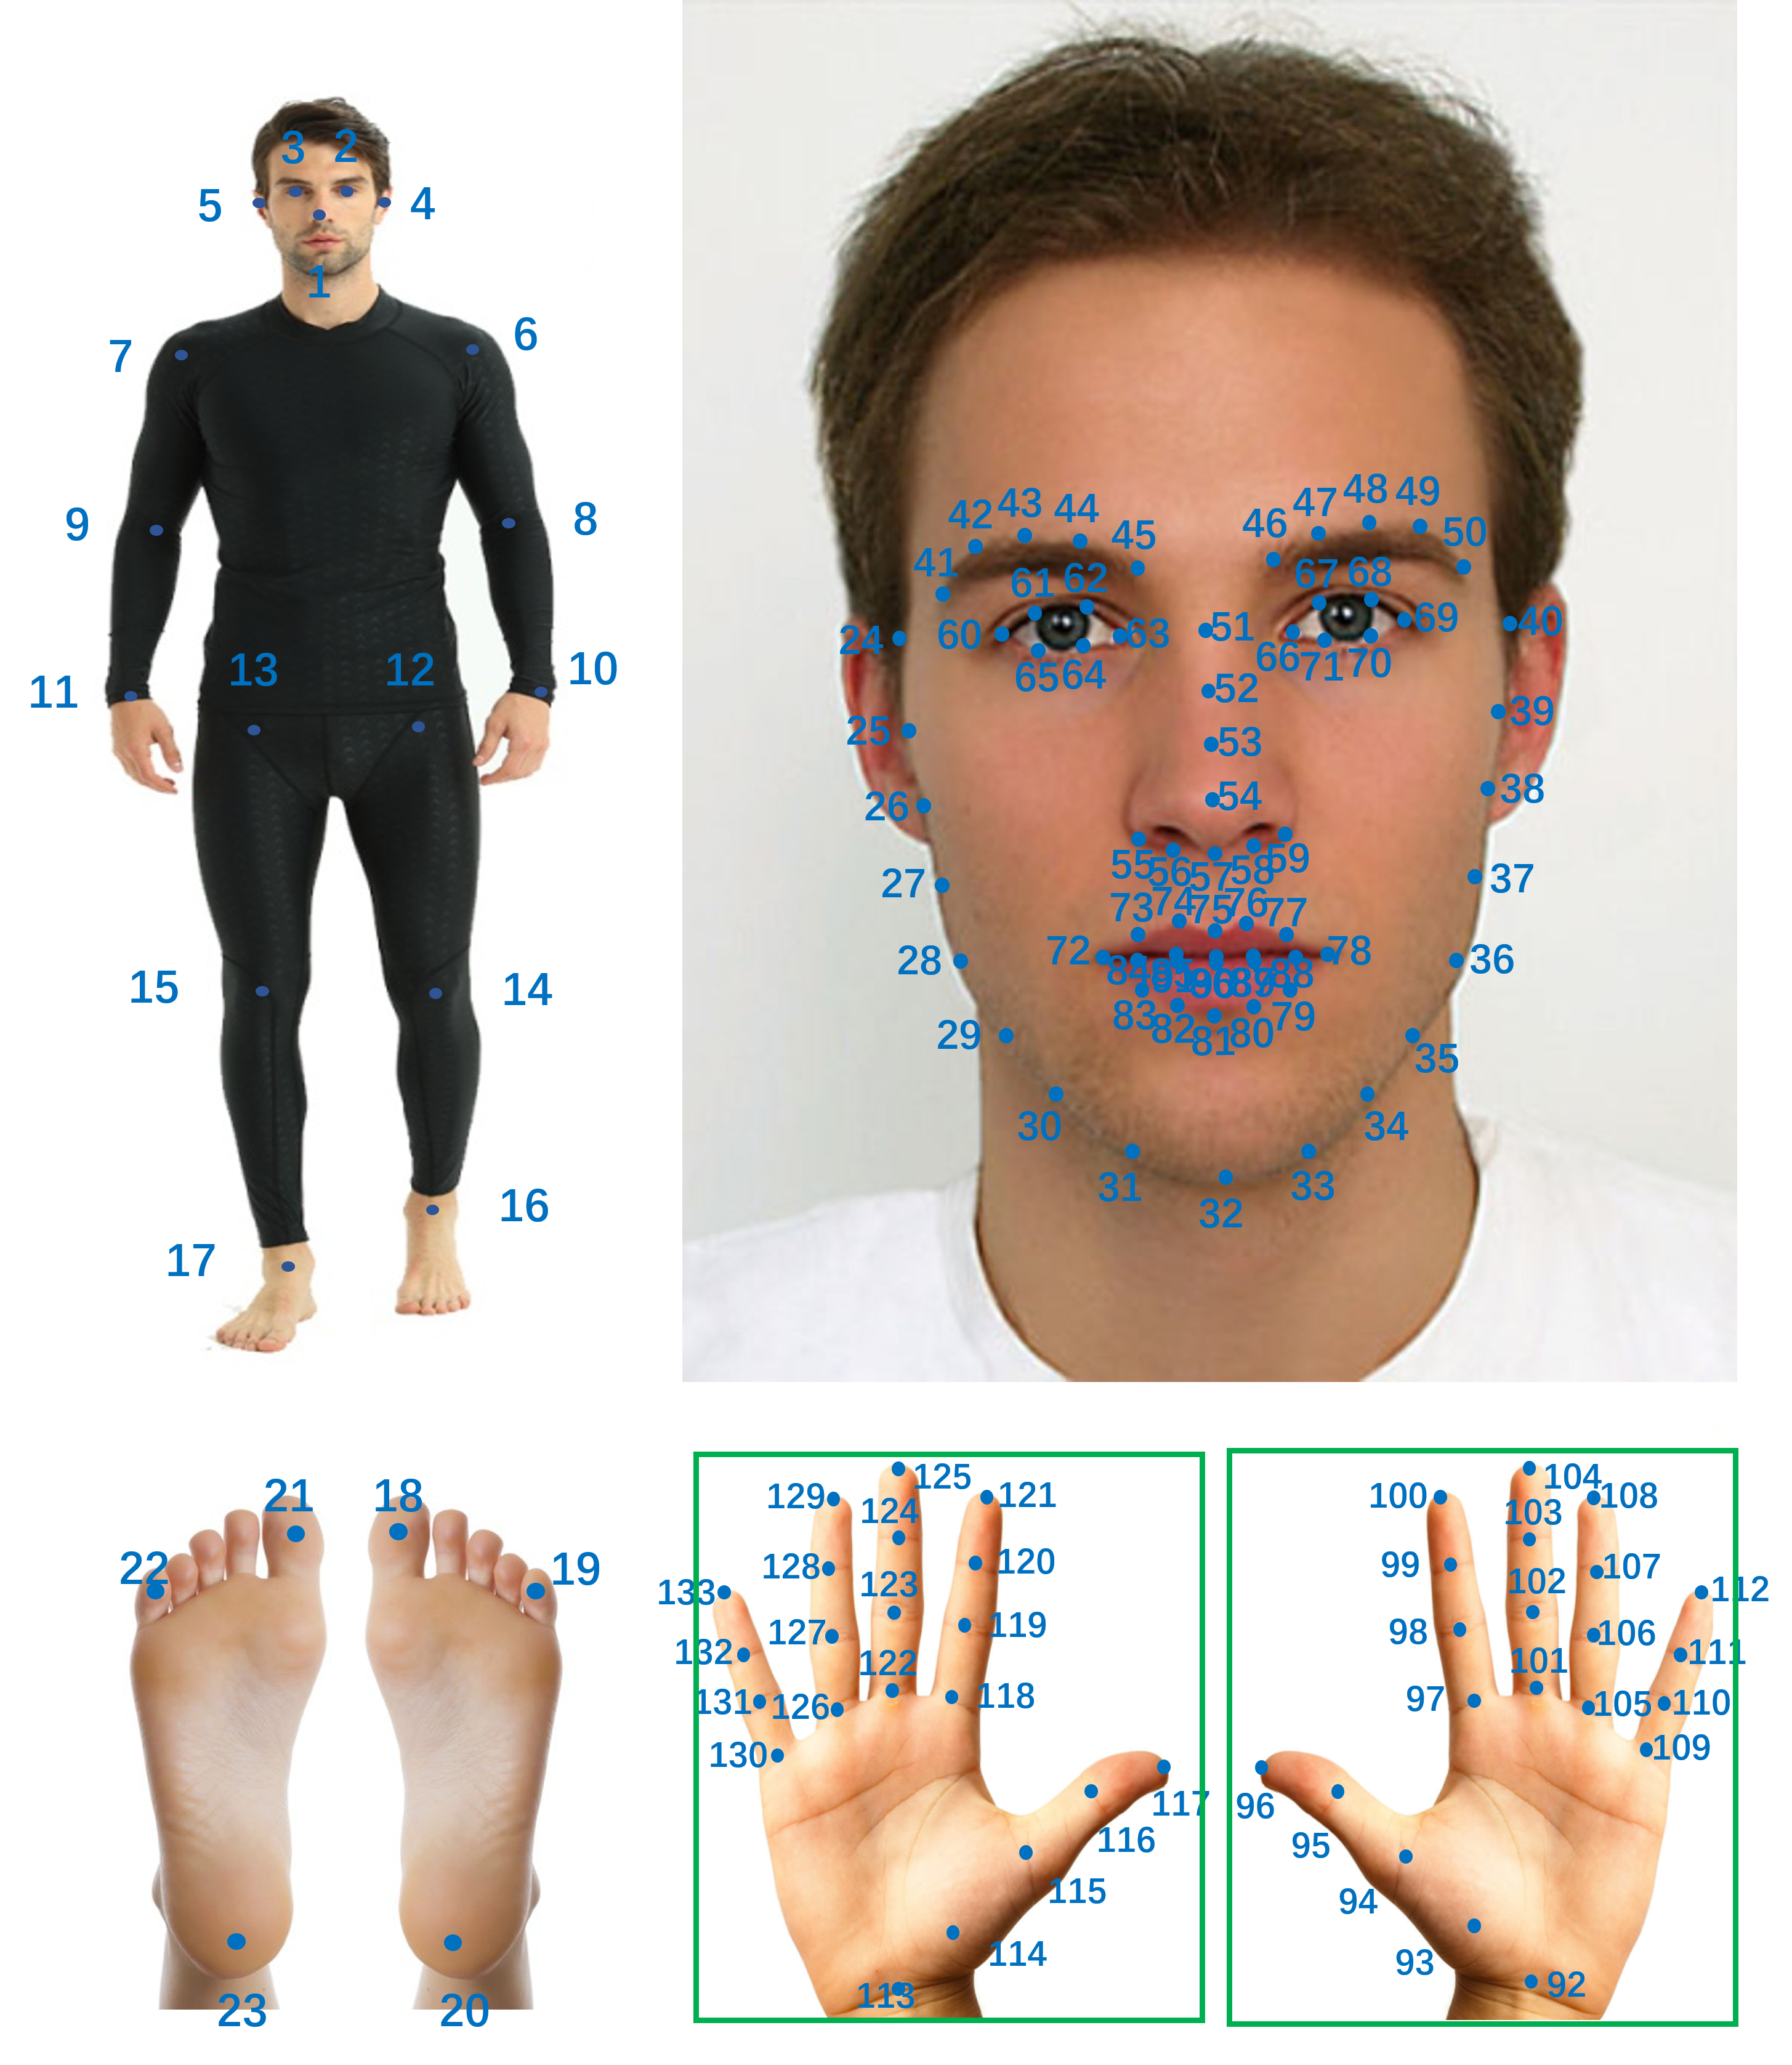
\includegraphics[width=\textwidth]{./m_figures/chapter1/other_model/coco.png}
        \caption{COCO~\cite{coco-wholebody} 格式参考}
        \label{fig:coco}
    \end{subfigure}
    \hfill  % 添加水平间距
    \begin{subfigure}[b]{0.35\textwidth}  % 修改宽度以适应横向排列
        \centering
        \includegraphics[width=\textwidth]{./m_figures/chapter1/other_model/openpose_25.png}
        \caption{Openpose~\cite{openpose} 格式参考}
        \label{fig:openpose}
    \end{subfigure}
    \caption{COCO 和 Openpose 格式参考}
    \label{fig:kp}
\end{figure}


MediaPipe中除了左右手21个关键点,和全身33个关键点的表示之外,对面部有更为详细的定义。
其面部由包括眼球、嘴部等部位在内的478个密集点进行定义,并给出了各点之间构成三角面片的组合关系,使其可进一步重建成网格表示,如图~\ref{fig:mediapipe} 所示。

相较于直接从视频中识别人体关键点,人体各部位均具有很强的结构化信息,可以利用深度学习或统计学方法从人体扫描数据建立基于网格的先验模型,并进一步通过参数控制的方式控制该先验模型,用以表征不同的人体形态和姿态,人体参数化模型表示具有更强的表示能力。
% 1.18 改到这一段
\begin{figure}[!htbp]
    \centering
    \begin{subfigure}[b]{0.9\textwidth}
        \centering
        \includegraphics[width=0.3\textwidth]{./m_figures/chapter1/other_model/m_body.png} \hfill
		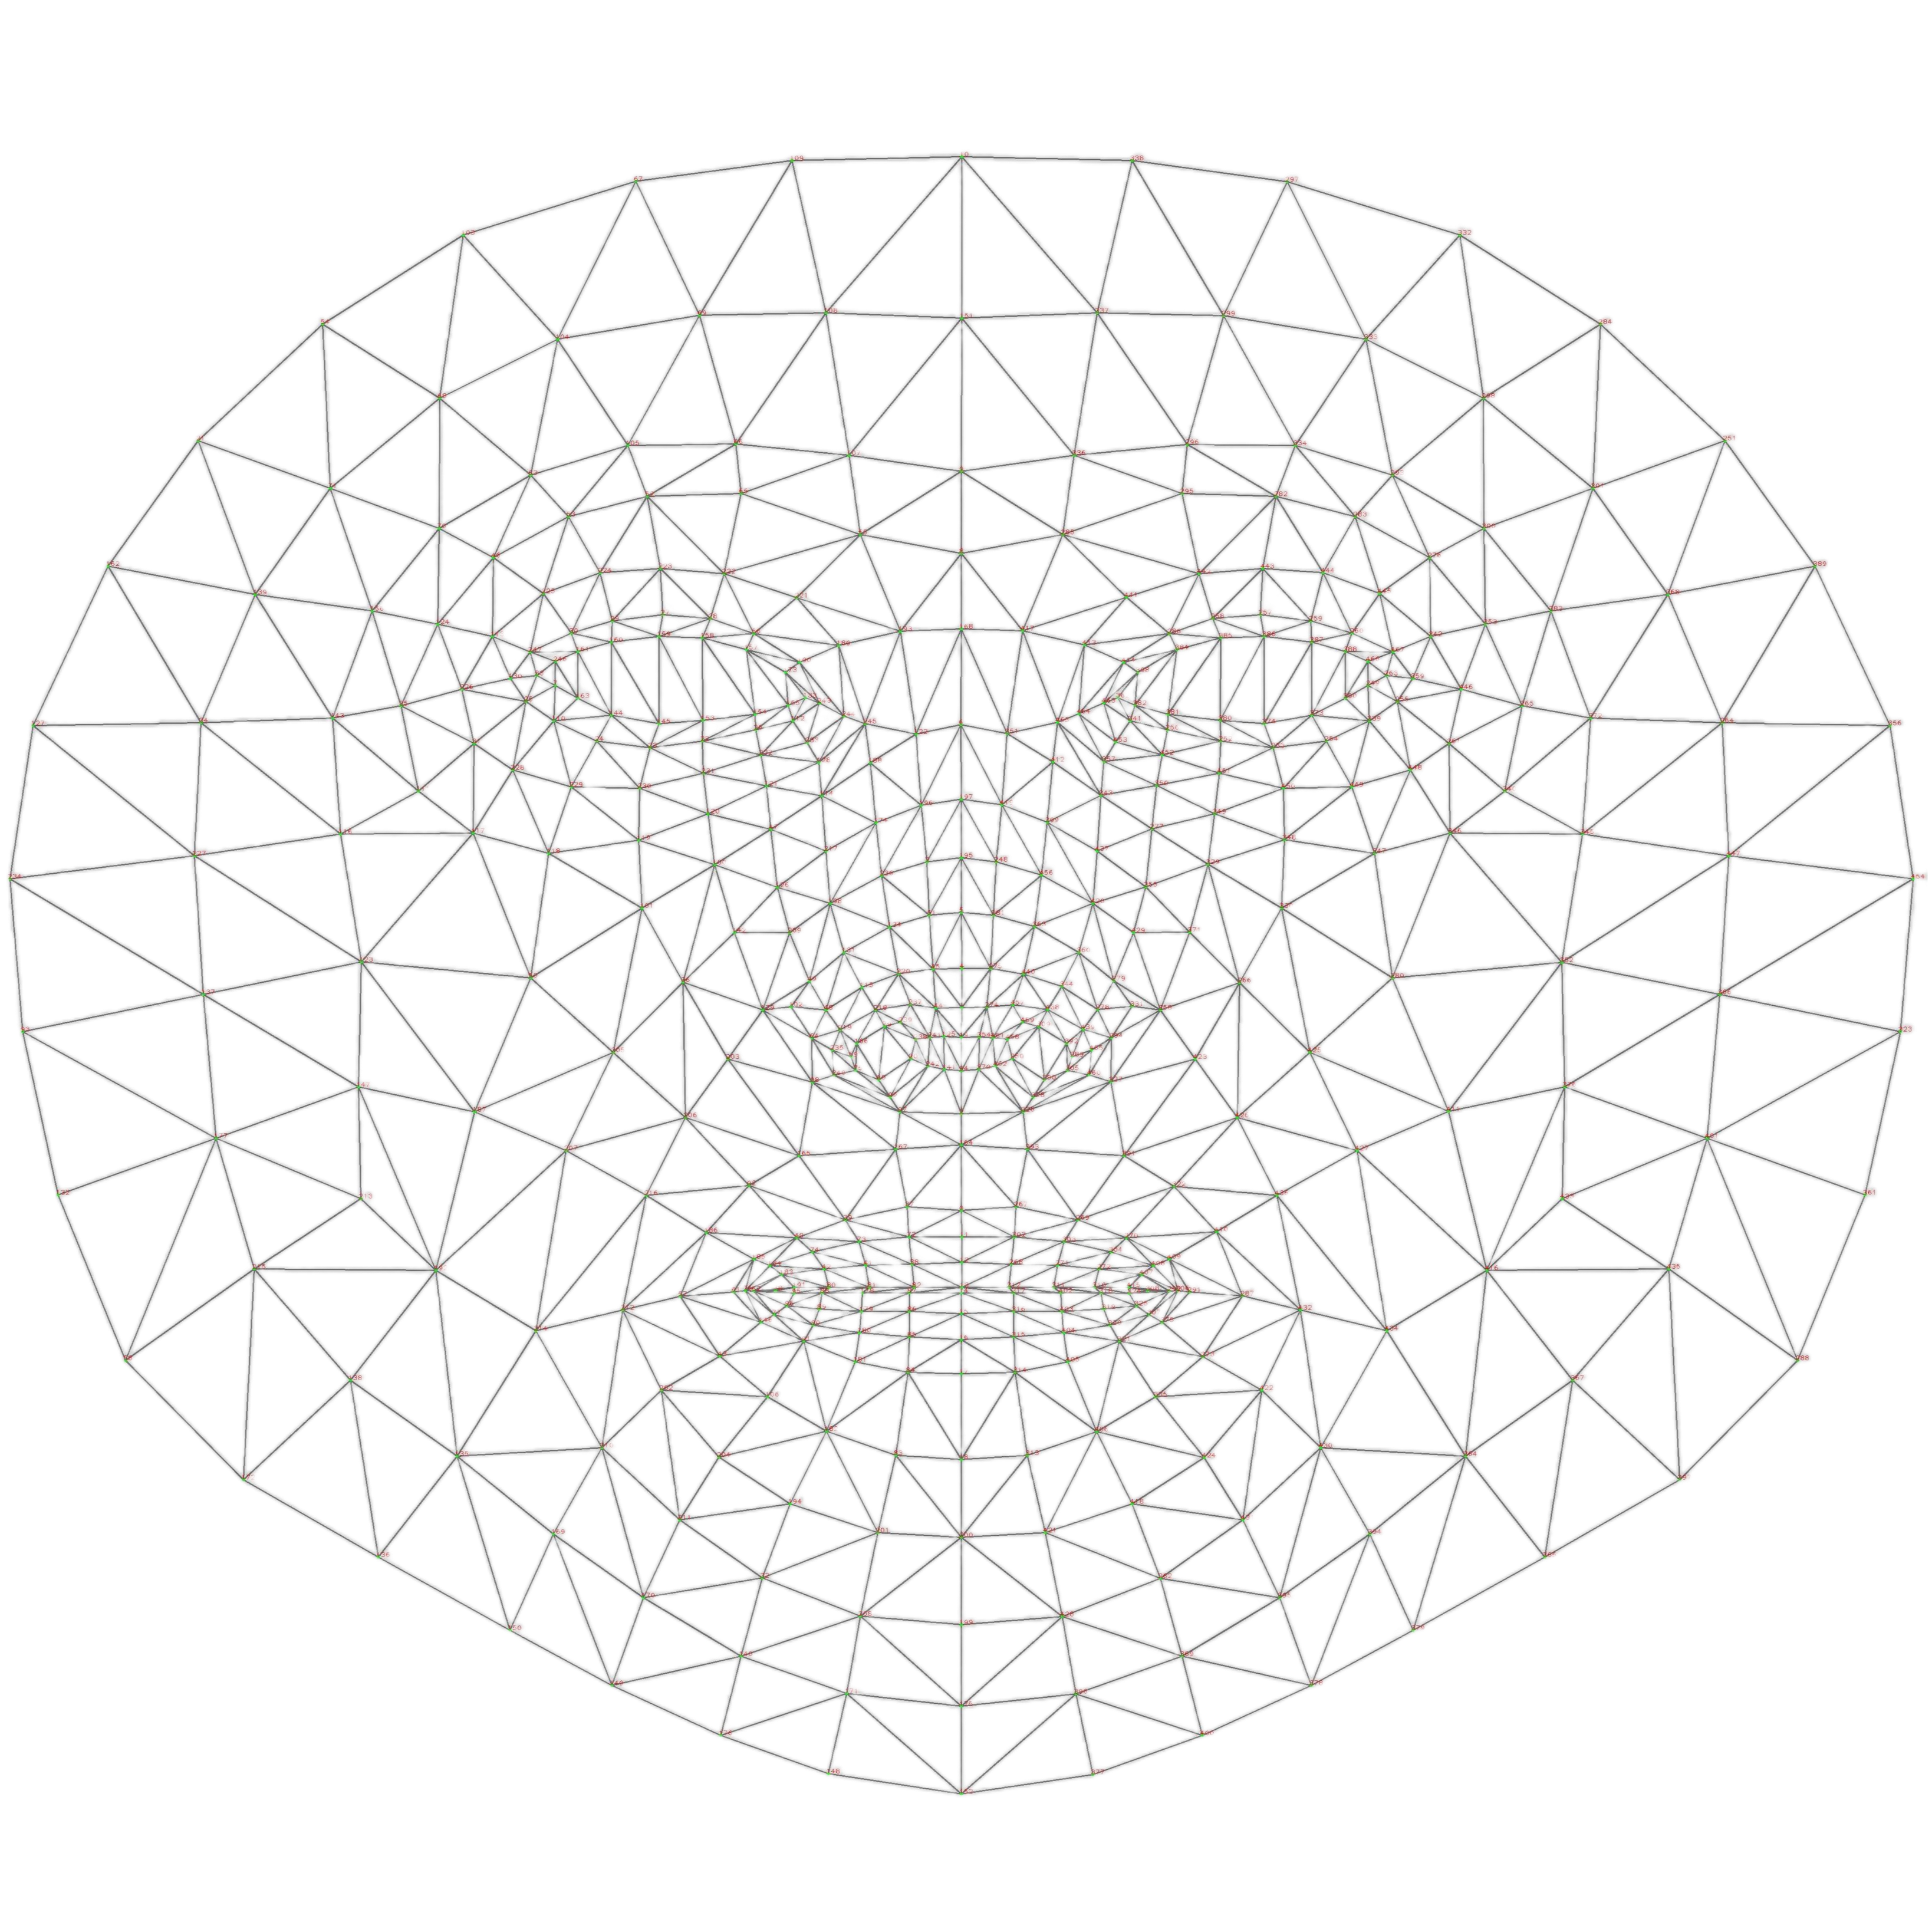
\includegraphics[width=0.3\textwidth]{./m_figures/chapter1/other_model/m_face.png} \hfill
		\includegraphics[width=0.3\textwidth]{./m_figures/chapter1/other_model/m_hand.png}
	\end{subfigure}
	\caption{MediaPipe~\cite{mediapipe} 格式参考}
	\label{fig:mediapipe}
\end{figure}

其中,三维人脸形变模型方法(3D Morphable Face Model,3DMM)\cite{3dmm}首次从三维人脸扫描数据中使用主成分分析方法构建参数化模型。该模型分别使用了表示面部形状和纹理的基向量。通过线性组合这些基向量,模型能够表示不同的三维人脸。一系列衍生方法在 3DMM 模型的基础上进行了拓展和改进,其中 LSFM 方法\cite{lsfm}进一步在模型中分解了人脸表情系数,构建了三维扫描表情数据集;
BFM 方法\cite{bfm}则在人脸模型当中引入了多尺度对称性,能够更细粒度的对人脸的细节变化进行控制;FLAME 方法\cite{FLAME:SiggraphAsia2017}进一步从人脸模型拓展到人头模型,在其中引入了姿态变量,能够进一步对人物头部转动、下颚张合、眼球转动等进行建模;Faceverse \cite{wang2022faceverse} 中利用从 Mediapipe\cite{mediapipe} 检测得到的关键点拟合得到相应的人脸模型系数,进一步提高了拟合速度。图~\ref{fig:3dmm}~展示了部分三维人脸形变模型。

\begin{figure}[!htbp]
    \centering
    \begin{subfigure}[b]{0.5\textwidth}
        \centering
        \includegraphics[height=3cm,width=\textwidth]{./m_figures/chapter1/3dmm/faceverse.jpg}
        \caption{Faceverse~\cite{wang2022faceverse} 模型}
    \end{subfigure}
    \hfill
    \begin{subfigure}[b]{0.45\textwidth}
        \centering
        \includegraphics[width=\textwidth]{./m_figures/chapter1/3dmm/bfm.png}
        \caption{BFM~\cite{bfm} 模型}
    \end{subfigure}
    \vspace{0.5cm}  % 增加竖直间距

	\begin{subfigure}[b]{0.9\textwidth}
        \centering
        \includegraphics[width=\textwidth]{./m_figures/chapter1/3dmm/flame.jpg}
        \caption{FLAME~\cite{FLAME:SiggraphAsia2017} 模型}
    \end{subfigure}
    \caption{各种3DMM模型示例}
    \label{fig:3dmm}
\end{figure}

针对手部的参数化模型最具代表性的工作是 MANO 模型\cite{mano},通过从大规模三维手部扫描数据中建立统计模型,其中基于PCA方法对手部形状建模,基于前向运动学树对手部姿态建模,MANO 模型通过形状参数 $\beta$ 和 姿态参数 $\theta $ 分别控制手部的静态形状和动作姿态。后续的工作如 HTML \cite{qian2020html} 将PCA分解后的纹理表示引入 MANO 模型当中;NIMBLE \cite{li2022nimble} 则结合肌肉和骨骼构建了针对手部的参数化模型。

针对全身的参数化模型,在工作\cite{allen2003space}中,首次将PCA分解应用于表示三维人体形态变化;SCAPE \cite{anguelov2005scape} 中将姿态形变模型引入参数化模型当中,
使得身体模型更具有真实肌肉形变感;在后续的工作\cite{allen2006learning} 则定义了标准线性蒙皮函数来建模姿态相关的形变;而SMPL \cite{smpl} 模型的出现使得参数化人体模型进一步被广泛使用。与 MANO 模型类似,SMPL模型的训练过程主要通过对大量的3D人体扫描数据进行分析,学习形状和姿态之间的关系。为了从3D扫描数据中提取出人体的统计特征,SMPL 也采用了PCA技术,将每个人体的形态表示为形状参数向量,并结合人体的前向运动学树来拟合具体姿势。具体来说,
SMPL\cite{smpl}  网格顶点由如下蒙皮公式(\ref{eq:smplM})控制。
\begin{equation}
    M(\beta, \theta) = W(T_P(\beta, \theta), J(\beta), \theta, W)
    \label{eq:smplM}
\end{equation}

其中,\(W(\cdot)\)表示混合蒙皮公式,\(\beta\)表示人体形状参数,\(\theta\)表示人体姿态参数,\(J(\beta)\)表示模型回归出的关节位置,\(W\)表示混合蒙皮权重。\(T_P(\beta, \theta)\)表示经过体和四肢变形后的人体模型顶点位置,由平均人体模板,形状以及姿态参数混合得到。
后续研究则在SMPL模型的基础上增加了手部、面部等信息,得到了更加生动的身体模型。SMPLH~\cite{smplh} 模型将 MANO 模型与SMPL 模型相结合,使得身体模型能够具有相应的姿态。
SMPLX~\cite{smplx} 在 SMPLH 的基础上进一步引入了 FLAME 模型,将面部动态变化也纳入身体模型当中。图\ref{fig:smpl} 展示了常用的身体模型。
\begin{figure}[!htbp]
    \centering
    \begin{subfigure}[b]{0.35\textwidth}
        \centering
        \includegraphics[width=\textwidth]{./m_figures/chapter1/other_model/smpl.png}
        \caption{SMPL~\cite{smpl} 模型}
    \end{subfigure}
    \hfill
    \begin{subfigure}[b]{0.3\textwidth}
        \centering
        \includegraphics[width=\textwidth]{./m_figures/chapter1/other_model/smplx.png}
        \caption{SMPLX~\cite{smplx} 模型}
    \end{subfigure}
	\hfill
	\begin{subfigure}[b]{0.3\textwidth}
        \centering
        \includegraphics[width=\textwidth]{./m_figures/chapter1/other_model/mano.jpg}
        \caption{MANO~\cite{mano} 模型}
    \end{subfigure}
    \caption{身体模型示例}
    \label{fig:smpl}
\end{figure}

\section{本文主要工作}

综上所述,随着近几年生成式人工智能的高速发展,生成式数字人工作层出不穷,出现了大量的不同的技术方案。但目前生成式数字人作为生成任务的子课题,仍处于探索阶段,目前现有的工作往往从可控性、生成速度、质量、连续性等多个方面探索如何提高生成式数字人的能力,并取得了可观的进展。但是由于人物视频数据的复杂性较高,且包含细粒度标注的视频数据集匮乏,在当前的研究工作中,如下4点局限性依然存在。

1) \textbf{可控性:}生成式数字人需要能够根据输入的动作、文本等多维度数据驱动对应的数字人形象,产生与驱动动作一致,且自然真实的人物视频序列。
然而,部分数字人技术\cite{liu2024anitalker,xu2024hallo}仅局限于单独的人物头像重演,缺乏自然的手势语言交互,缺乏真实感。
部分数字人技术\cite{lin2024cyberhost}仅从音频输入中驱动人物形象,缺乏对人物肢体的控制。
因此为了提高生成式数字人模型对驱动信息的可控性,需要提高驱动模态的有效性和模型对驱动信息的理解能力。

2) \textbf{生成速度:}生成式数字人对于生成速度也存在要求。视频合成实时率用来描述视频合成耗时与输出视频时长比值。
我国《数字虚拟人技术要求》\cite{数字虚拟人技术要求}中要求生成的数字人视频需要不低于25帧每秒,同时在1080分辨率条件下,合成实时率需小于1。
这个要求的提出是因为数字人任务往往需要应用于直播、在线客服等实时领域。而基于扩散模型及 Transformer 架构的生成式数字人模型虽然能够合成高质量的数字人,但其往往需要数十倍于视频时长的生成时间。
难以满足生成式数字人的生成速度要求。同时较长的生成时长也存在明显的产品控制风险,如当进行离线的长时间的数字人节目生成时,冗长的制作周期,使得在制作过程中难以对其中的问题片段进行调整。

3) \textbf{生成质量:}生成式数字人需要能够生成高保真的写实数字人视频序列。
尤其是生成画面细节的丰富度和逼真度。生成式数字人模型最终生成的图像结果不仅需要能够生成嘴部,头部,躯干等主体内容,也需要能够重现眨眼,头发,手部等细微特征的表达,细微表达的缺少会导致生成视频效果呆板,真实性和表现力的下降。

4) \textbf{时序一致性:}生成式数字人需要能够生成具有时序一致性的数字人帧序列。
该连续性包括了数字人动作一致性和视频帧间的一致性。其中动作一致性一般包括人物动作连贯一致,无跳变等方面,而视频一致性则一般包括帧间的过渡效果,画面流畅性等方面。
因此相比于图像生成任务,视频生成任务需要额外考虑帧间的时序建模问题。时序一致性差可能表现为伪影、画面色彩抖动和数字人动作不自然,不规则运动等问题。

因此,本文主要工作围绕生成式数字人领域目前存在的局限性进行研究和改进。提出了基于多维度特征融合的生成式数字人解决方案。首先,本文提出了基于多维度特征的基准数据集构建方法,整合集成了多种关键技术,实现从单目视频数据中提取高质量多维度合成人体数据表征,该合成图像表征能精确的表征数字人的嘴型、眼部、手部及躯体动作,并利于神经网络模型建模。

接着针对该解决方案,以条件式对抗生成网络为基础架构具体实现多维度特征融合的数字人建模。并进一步在该框架下针对数字人生成任务的整体形象和细节表示引入了基于人体大模型的损失函数和基于数字人任务判别器结构优化。从这两个方面实现全局维度特征和局部维度特征的融合。针对生成过程中的时序一致性,本文在当前数字人模型中引入了基于帧间连续特征的时序特征融合方法方法和基于多任务学习的法线特征融合方法。

最后本文整合了驱动与呈现的相关技术方案,以数字人下游实际的应用为例,阐明数字人实际解决方案。利用建模完成的数字人模型,实现了对上述改进方案的验证。

具体来说,本文的主要工作如下:

1) 数字人基准数据集构建方法。该方法从数据的角度出发,解决数字人生成任务中数据匮乏和不一致的问题,提出了一个基于多维度融合的数据集构建流程,整合了多种关键技术,实现了从单目视频数据中提取高质量多维度合成数字人数据样本,构建的合成图像特征能精确的表征数字人的嘴型、眼部、手部及躯体动作,并利于神经网络模型建模。该工作针对性的解决了生成式模型的可控性问题。

2)数字人局部细节和整体形象增强的改进。针对生成式数字人任务,提出基于多维度特征融合的条件对抗生成网络基本架构,该架构能够实时、可控的生成高保真数字人视频。并进一步设计并实现了基于人体大模型的损失函数和基于数字人任务的局部判别器结构。分别从整体形象和局部细节增强数字人建模效果。其中基于条件对抗式生成的模型有效解决了生成速度问题,满足了实时性应用的要求;而针对数字人任务的模型优化则进一步提高了生成质量。

3) 基于帧间连续性和法线约束的时序一致性改进。分别提出基于法线约束的多任务学习方法和基于多帧时序连续性的时序增强方法。前者通过跨帧几何一致性,后者通过连续帧条件约束,均有效提升了生成数字人视频生成的时序一致性。同时结合本文数字人基准数据集构建方法,设计了时序一致性闭环检测方法,用以对生成式数字人视频的时序一致性进行评估。该工作针对时序一致性提出并实现了可行的解决方案,并进一步提出在数字人任务上的时序一致性衡量标准。

4) 基于多维度特征融合的生成式数字人应用案例。本文首先阐明了本文模型在推理驱动阶段时的数据通路,并结合生成式数字人应用案例,进一步阐明了本文所提出的生成式数字人方法如何与其他技术进行结合进行驱动呈现,验证了本文提出的生成式数字人建模方案的可行性。

\section{本文章节安排}

本文章节组织结构如图 \ref{fig:framework} 所示,由如下六个章节组成:
\begin{figure}[!htbp]
	\centering
	\includegraphics[width=0.6\textwidth]{./m_figures/chapter1/框架.pdf}
	\caption{论文结构图}
	\label{fig:framework}
\end{figure}

第 1 章:绪论。该章节介绍了本文的研究背景和研究意义,论述了目前相关的研究工作和数字人生成领域存在的问题,明确了本文主要的工作内容和相关贡献,最后给出文本的结构安排。

第 2 章:生成式数字人中的多维度特征融合总体方案。该章节从宏观的角度概述了本文数字人基于多维度融合的数字人建模方案的总体方案,详细阐述以人为中心的多维度训练集构建流程,并深入分析了本文构建的各模态信息在生成式数字人建模任务的用途。本文构建的合成图像特征能精确的表征数字人的嘴型、眼部、手部及躯体动作,并利于神经网络模型建模。并进一步利用该建模方法构建本文的基准数据集,并针对数字人生成任务,阐明相关的评估指标。

第 3 章:全局人体特征和局部位置特征的融合增强方法。本文以 StyleUNet\cite{styleAvatar} 为实现基准方案,构建了能够融合多维度特征的数字人建模方法。在该框架下针对数字人生成任务的整体形象和细节表示引入了基于人体大模型的损失函数和基于数字人任务的局部判别器结构优化。从这两个方面实现全局维度特征和局部维度特征的融合。

第 4 章:帧间连续性与法线属性融合的时序一致性改进。该章节在上一章实现的基准模型上,分别探索了两条改进路线;即基于法线约束的多任务学习方法和基于连续帧的时序融合方法。分别从几何一致性和帧间时序连续性的两个角度对生成式数字人进行了改进,提升生成数字人视频的时序一致性。最后,本文设计了一套数字人时序一致性闭环检测方法,利用该检测方法,对本章节中的改进在数字人动作时序一致性上进行了评估实验和结果分析,并将最终改进的模型与其他开源模型进行了性能对比。

第 5 章:生成式数字人应用案例。该章节针对数字人驱动呈现任务,首先阐明本文模型在推理时的数据通路,并将建模完成的数字人应用于实际系统当中,进一步阐明了基于本文提出的多维度特征融合的生成式数字人应用方案和具体的交互流程。

第 6 章:总结和展望。该章节对全文工作进行了回顾和总结,提炼了本文的重点工作成果,并对本文工作的局限性及未来可能的改进方向进行了展望。

% \chapter{数字人基准数据集构建方法}
% 
当前的生成式数字人方法缺少统一的数据处理标准,使得在构建完整的数字人解决方案时,
往往需要根据所使用的基础模型,修改对应的数据预处理方法;并且当驱动模态发生变化时,也难以对方法进行公平比较。
如在 Animate anyone\cite{hu2024animate} 数字人视频生成模型中,
模型使用基于DWpose\cite{dwpose} 绘制的身体点线图作为驱动模态,在 Champ\cite{zhu2024champ} 中,
额外使用了 SMPL\cite{smpl} 模型的法线图、语义图、深度图加以融合。在Magicanimate\cite{magicanimate}中,
则使用Densepose\cite{guler2018densepose} 渲染图作为驱动模态。
因此本文提出了一种细粒度高质量的以人为中心的数据预处理流程,用以从人物视频数据集当中提取包含全身多部位细粒度的合成模态数据,并进一步分析了提取出的合成模态表征能力。%该数据处理方法和生成的多维度数据集为多维度驱动的数字人生成模型提供了。

\section{概述}
在生成式数字人任务当中,现有开源的单目视频数据在分辨率、帧率设置,其采集质量、和背景信息中均存在很大差异。另一方面这些原始视频数据中缺乏模型能够直接使用的和经过标注和清洗的信息。因此在本文中,针对单目人物视频数据,构建了一套全流程的多维度数据集处理方法,并对本文所使用的数据集和数字人模型质量评估方法进行介绍。

本文聚焦于通过多维度数据生成数字人视频序列,因此需要能够高效准确的从单目视频获取所需的多维度数据,并进一步对原始视频帧进行优化。结合当前相关人体任务研究成果,本文提出了一种自动化的多维度数字人数据集构建方法,用以从任意单目全身视频中提取数字人训练素材。简单来说可以将数据集构建流程分为以下五个步骤:

\textbf{1)数据自动化清洗和分割}

将原始视频数据处理成以人物为中心的 1024\(\times\)1024 分辨率的视频,调整其帧率为 25 帧每秒 。并利用每帧检测的 MediaPipe\cite{mediapipe} 检测结果,将人物视频切分为若干人物片段。利用该方式能够去除视频当中非人物帧、存在质量问题和面部显示不完整的视频片段。
最后利用 Arcface\cite{deng2019arcface} 将所有视频根据人物的身份特征进行聚类。此步骤旨在对数据进行初步的清洗和人物身份分类。
    
\textbf{2)全身关键点检测}

利用 Mediapipe\cite{mediapipe}, DWpose\cite{dwpose} 等方法对步骤一中得到的预处理视频片段进行全身关键点检测,分别获取脸部、眼部、躯干的 landmark ,并进行时序平滑处理。此步骤旨在利用检测算法提供的关键点为后续前景分割和人体先验模型拟合提供基础。
    
\textbf{3)人物前景分割}

利用上一步骤中关键点作为提示标记人物对象在图中的位置,指导 SAM2\cite{sam2} 进行掩码分割,将任意视频中的人物与其背景分离。针对掩码过程中可能存在的噪点等问题,通过形态学算法和最大流方法进行进一步清洗。该步骤旨在利用掩码生成绿幕背景视频序列。

\textbf{4)人体先验模型拟合}
    
分别利用 Faceverse\cite{wang2022faceverse}, AiOS~\cite{sun2024aios}, HaMeR~\cite{hamer} 等方法提取人物视频中的 Faceverse 面部表示,
全身 SMPLX~\cite{smplx} 表示,手部 MANO~\cite{mano} 表示,及相应的相机姿态。针对AiOS全身识别中手部不准确的情况,利用更准确的 HaMeR 识别结果对其校准。对于相机姿态,和各姿态表示使用平滑算法进行平滑。该步骤旨在存储人体先验模型参数,为最终多维度图像绘制提供基础。

\textbf{5)合成数据生成}

通过将各人体先验模型将对应的系数映射成网格顶点,并回归出关节点,分别绘制 SMPLX 语义图,法线图,深度图以及 MANO 手部图。利用 OpenGL 将关节点和面部 Mesh 顶点绘制成神经语义图像序列。将面部顶点对应的眼部关键点绘制成眼部注视图像。该步骤旨在得到最终的模型多维度输入数据。

经过上述步骤。单目人物视频数据即被处理为高质量、细粒度标注的数字人多维度数据集。具体来说,该数据集被存储为如下数据格式:真实图像文件,关键点标注文件,绿幕背景图像文件,二值掩码文件,
SMPLX~\cite{smplx} 系数文件,MANO~\cite{mano} 系数文件,Faceverse~\cite{wang2022faceverse} 系数文件,CCBR 图像文件,眼睛注视图像文件,SMPLX 语义图像文件, SMPLX 法线图像文件,
MANO 手部图像文件。其总体的流程与各模态数据格式示例如图~\ref{dataset_pipeline}~所示。
\begin{figure}[!htbp]
	\centering
	\includegraphics[width=0.9\textwidth]{./m_figures/chapter2/数据集处理绘图.pdf}
	\caption{数据处理流程及数据存储格式}
	\label{dataset_pipeline}
\end{figure}

\section{数据自动化清洗和分割}

数据清理与分割的核心目标是提升数据集质量,减少如噪声、缺失的人物帧等不良信息对模型性能的负面影响。保证每段视频中的人物形象和动作相对稳定。

对于采集的原视频,读取其元数据中包含的信息,并过滤掉低于预设阈值的视频,避免低分辨率数据对模型训练的影响。分辨率达标的视频使用 MediaPipe\cite{mediapipe} 工具对视频逐帧检测得到对应的全身关键点和对应点置信度。通过MeidaPipe每帧是否检测成功标记人物的完整出现区间,识别并提取具有完整人物的起始帧和结束帧。经过该处理,将每个视频被切分为若干人物片段。

对提取的每段人物片段,进行裁剪操作。假设在第一帧中检测到的人物关键点集合为:\(K = \{(x_i, y_i)\}_{i=1}^N\)其中 \(N\) 为关键点总数。
遍历得到关键点的最小坐标值\(x_{\text{min}}\), \(x_{\text{max}} \)和最大坐标值\(y_{\text{min}} , y_{\text{max}}\)。
接着根据最小和最大坐标值,计算包围盒的初始宽度和高度,如公式(\ref{eq:center})所示:
\begin{equation}
(x_c, y_c) = \left(\frac{x_{\text{min}} + x_{\text{max}}}{2}, \frac{y_{\text{min}} + y_{\text{max}}}{2}\right)
\label{eq:center}
\end{equation}

选取包围盒的长边\(L\)作为方形裁剪区域的边长,并按照一定的比例拓展,以确保覆盖整个人物。考虑拓展比例 \(\alpha > 1\),拓展后的裁剪区域边长如公式(\ref{eq:length})所示。
\begin{equation}
L = \max(w_{\text{box}}, h_{\text{box}}), L' = \alpha L
\label{eq:length}
\end{equation}

如果拓展后的包围盒超出视频底边,则调整包围盒中心坐标向上移动,直至其完全处于视频范围内。
此时假设视频高度为 \(H\),\(\text{若 } y_c + \frac{L'}{2} > H, \quad \text{则 } y_c = H - \frac{L'}{2}\)对于除底边外其他超出视频范围的部分,使用绿幕色背景进行填充,
其RGB值为$[0, 177, 64]$。最后,裁剪区域的范围可被定义为公式(\ref{eq:box})所示。
\begin{equation}
    \begin{split}
    (x_{\text{crop,min}}, y_{\text{crop,min}}) &= \left(x_c - \frac{L'}{2}, y_c - \frac{L'}{2}\right) \\
    (x_{\text{crop,max}}, y_{\text{crop,max}}) &= \left(x_c + \frac{L'}{2}, y_c + \frac{L'}{2}\right)
    \end{split}
    \label{eq:box}
\end{equation}

最终得到的方型裁剪区域采用双线性插值方法缩放至 $1024\times1024$ 的标准分辨率,并使用 25 帧每秒的视频速率进行下采样,生成统一规格预处理视频,确保数据输入的规范性与统一性。

最后使用 ArcFace 方法\cite{deng2019arcface},从预处理视频中的第一帧人脸中提取身份特征对人物进行聚类,存入特定身份的数据目录。通过上述处理流程,基本实现了对原始视频数据的初步清洗过滤,并按照不同人物身份进行划分,为后续多维度数据集构建提供了高质量的基础素材。

\section{全身关键点检测工具}

从视频帧中进行关键点的提取,是对视频中的人物进行建模的第一步。本文分别用 MediaPipe\cite{mediapipe} 和 Dwpose\cite{dwpose} 提取视频帧中的面部和身体关键点及其置信度。MediaPipe 能提供准确且细粒度面部顶点标注,而 Dwpose 在身体关键点的识别上更准确。具体来说, MediaPipe 方法用以提取面部共 478 个关键点,该关键点除像素平面的$(x,y)$坐标外,还具有预测的伪深度坐标 $z$。Dwpose 则分别提取身体 23 个二维关键点,以及双手共 42 个二维关键点。面部和全身关键点均具有置信度。

为了减少提取关键点在时序上的抖动,本文利用一欧元滤波器 \cite{casiez20121} 对关键点进行平滑处理,减少各帧间检测噪音导致的小幅度抖动。同时对于部分检测结果缺失的视频帧,利用视频帧上下文,采用线性插值的方式对可能缺失的关键点进行补全。
处理后的全身关键点将作为标签点提示SAM2 \cite{sam2}进行人物前景分割;Faceverse \cite{wang2022faceverse} 方法中使用 Mediapipe 面部关键点拟合得到人物各帧面部系数;手部关键点及其置信度将用以 HaMeR \cite{hamer} 方法中包围盒的确定和用以辅助手部神经语义图像绘制。

\section{人物前景分割工具}

人物前景分割通过对人物视频帧进行背景剔除,能够消除背景对生成结果的干扰,
使得后续模型在建模过程中不必要去学习复杂的背景生成,从而进一步提高数字人生成任务的生成质量。在该部分,
本文使用 SAM2~\cite{sam2} 从视频中进行人物前景分割。

SAM2 基于提示编码器、记忆注意力层和记忆编码器的架构设计能够有效处理遮挡问题,并将前序掩码在时序中进行传播,完成复杂的视频跟踪分割任务。 该模型中的提示编码器用以处理输入的提示信息。具体来说点、框、文本等多维度提示都可用于指导模型分割图像中的特定对象。通常 SAM2 采用的是交互式分割的方法,即模型将用户传入的标记点作为提示来选择和细化目标对象,模型会根据这些提示自动将分割传播到视频的后续帧。本文基于该种方式进行拓展,通过识别的关键点进行自动化的人体前景风格。


在实际处理中,为了防止预处理视频过长,导致人物追踪失效,将预处理视频片段首先划分为25秒总500帧的子片段。
将每个子片段中的第一帧中识别并存储的关键点中选择Dwpose中的 12 个主要躯干关键点加上 1 个面部鼻子部位关键点作为人体前景标记点。进一步,为了防止处理时物体遮挡导致的分割错误,对标记点置信度进行遍历判断,保留置信度超过阈值的点。传入给 SAM2 的提示编码器,用以标记视频中的人体对象前景。通过该方法能够很好使得SAM2分割出人体对象。


% 在实际处理中,为了防止预处理视频过长,导致人物追踪失效,将预处理视频片段首先划分为25秒总500帧的子片段。将每个子片段中的第一帧中识别并存储的关键点中选择如表\ref{tab:dwposeindex}所示的12个躯干关键点加上1个面部鼻子部位关键点作为人体前景标记点。进一步,为了防止处理时物体遮挡导致的分割错误,对标记点置信度进行遍历判断,保留置信度超过阈值的点。传入给 SAM2 的提示编码器,用以标记视频中的人体对象前景。通过该方法能够很好使得SAM2分割出人体对象。

% \begin{table}[!htbp]
%     \centering
%     \begin{tabular}{cc|cc|cc}
%     \toprule
%     \textbf{索引} & \textbf{部位名称} & \textbf{索引} & \textbf{部位名称}& \textbf{索引} & \textbf{部位名称}\\   
%     \midrule
%     0 & 鼻子 & 5 & 左肩膀 & 6 & 右肩膀 \\
%     7 & 左肘部 & 8 & 右肘部 &  9 & 左手腕 \\
%     10 & 右手腕 & 11 & 左臀部 & 12 & 右臀部 \\
%     13 & 左膝部 & 14 & 右膝部 & 15 & 左踝部 \\
%     16 & 右踝部 \\
%     \bottomrule
%     \end{tabular}
%     \caption{对应Dwpose关键点索引及部位}
% \label{tab:dwposeindex}
% \end{table}

直接通过该方法得到的二值背景掩码可能会存在噪点问题,并且人物边缘可能存在背景缝隙,因此还需要进一步对掩码进行处理。
首先通过形态学腐蚀操作断开可能与人体掩码相连的噪点,并且减少可能在人物边缘可能存在的背景缝隙。此时进一步将掩码当中的中最大连通分量作为人物掩码。最终可得到如图~\ref{fig:sam2_2}~所示的掩码。

为了进一步对掩码边缘进行平滑,减少边缘锯齿,将二值掩码拓展为范围从 0 到 255 灰度掩码,对该灰度掩码进行高斯滤波处理。
本文将背景处理成RGB色彩为$[0, 177, 64]$的绿幕背景。将该灰度掩码融合回原图时,对于掩码边缘,使用灰度值混合绿幕背景和原始视频信息。
当完成掩码融合后,得到最终的人物前景分割图像,如图~\ref{fig:sam2_3}~所示。此时分别将未经过灰度变换和平滑处理的掩码和人物前景分割图像进行存储。

\begin{figure}[!htbp]
    \centering
    \begin{subfigure}[b]{0.3\textwidth}
        \centering
        \includegraphics[width=\textwidth]{./m_figures/chapter2/sam2/origin.png}
        \caption{原始视频图像}
        \label{fig:sam2_1}
    \end{subfigure}
    \hfill
    \begin{subfigure}[b]{0.3\textwidth}
      \centering
      \includegraphics[width=\textwidth]{./m_figures/chapter2/sam2/sam2.png}
      \caption{SAM2 掩码示例}
      \label{fig:sam2_2}
    \end{subfigure}
    \hfill
    \begin{subfigure}[b]{0.3\textwidth}
      \centering
      \includegraphics[width=\textwidth]{./m_figures/chapter2/sam2/sam_final.png}
      \caption{SAM2 掩码叠加结果}
      \label{fig:sam2_3}
    \end{subfigure}
    \caption{SAM2~\cite{sam2} 结果图}
    \label{fig:sam2}
\end{figure}


\section{人体先验模型拟合}

人体先验模型拟合进一步利用人体先验模型提取单目人物视频中的人体数据并进行重构。

\textbf{1)面部模型拟合}

首先本文利用Faceverse~\cite{wang2022faceverse} 利用 Mediapipe~\cite{mediapipe} 中 478 个关键点作为伪真值拟合人物的面部系数。针对序列中的一帧人物数据 $I \in \mathbb{R}^{W\times H\times C}$ 而言,
面部系数包括形态系数$\beta\in \mathbb{R}^{150}$、表情系数$exp \in \mathbb{R}^{52}$、姿态系数$\theta \in \mathbb{R}^{3} $ 、相机位移系数$trans \in \mathbb{R}^{3} $等。此时全脸关键点由$ID$、$exp$、$rot$、$eye$、$trans$等系数共同决定。$base_{id}$ 是Faceverse的身份基向量,$base_{exp}$ 表情基向量,$base_{mean}$是Faceverse的平均关键点。
通过式(\ref{eq:faceverse})线性组合得到完整的人脸顶点映射表示$V_{shape}$:
\begin{equation}
  \begin{split}
    V_{shape} = base_{id} \times ID + base_{exp} \times exp + base_{mean}
  \end{split}
  \label{eq:faceverse}
\end{equation}

最后利用与 Mediapipe 中对应的478个关键点索引,获得稀疏表示的 Faceverse 面部顶点。

\textbf{2)手部模型拟合}

本文利用 HaMeR\cite{hamer}  提取人物基于 MANO 模型\cite{mano}的手部系数。具体来说针对每只手,
其提取的系数包括全局转动系数$rot \in \mathbb{R}^{3} $、姿态系数$\theta \in \mathbb{R}^{45}$、形态系数$\beta\in \mathbb{R}^{10}$和相机位移$trans \in \mathbb{R}^{3} $。而后使用 MANO 平均关键点和对应的表面蒙皮函数重建得到表面顶点。

此外,在原始的 HaMeR 推理管线中,其依赖于 VitPose\cite{xu2022vitpose} 提取的手部关键点确定手部包围盒并识别左右手信息,并根据关键点置信度阈值判断该帧手部是否真实存在,仅重建达到阈值的手部。本文将该过程修改为直接使用步骤二中 Dwpose\cite{dwpose} 的关键点信息,更高效的利用已有的提取结果,降低处理成本。

\textbf{3)全身模型拟合}

本文使用 SMPLX模型\cite{SMPL-X:2019} 对于全身系数的提取。
具体来说,其包括了手部姿态系数$\theta_\text{hand} \in \mathbb{R}^{90}$,
头部姿态系数$\theta_\text{head} \in \mathbb{R}^{9}$,身体姿态系数$\theta_\text{body} \in \mathbb{R}^{63}$,
面部表情系数$exp \in \mathbb{R}^{10}$,形态系数$\beta\in \mathbb{R}^{10}$,相机位移$trans \in \mathbb{R}^{3} $。当得到系数,同样使用对应的 SMPLX 蒙皮函数和平均关键点得到对应参数状态下的网格关键点并回归出对应的全身共144个身体关节点。

为了得到相对准确的全身表示,本文选取了一段15秒总375帧的自采集人物动作片段,分别对比 
Smpler-X\cite{cai2024smpler}, OSX \cite{lin2023one},
multi-HMR\cite{multi-hmr2024},AiOS~\cite{sun2024aios} 进行 SMPLX 拟合结果。
其结果可视化对比表明,Smpler-X 和 OSX 不能够很好拟合人物的动作,在全身尤其是手部动作上存在较大的差距。而 multi-HMR 虽然全身拟合结果很好,但从时序结果上观察存在剧烈的手部抖动。而 AiOS 可视化结果与 multi-HMR 相当,但是在时序上效果更加平滑,因此相对其余三个模型更好。图~\ref{fig:smplx_result}~展示了四种方法在同一帧中的检测表现。本文最终使用 AiOS 提取全身先验。

\begin{figure}[!htbp]
    \centering
    \begin{subfigure}[b]{0.24\textwidth}
        \centering
        \includegraphics[width=\textwidth]{./m_figures/chapter2/smplx/smpler2.jpg}
        \caption{Smpler-X\cite{cai2024smpler} 结果}
    \end{subfigure}
    \hfill
    \begin{subfigure}[b]{0.24\textwidth}
        \centering
        \includegraphics[width=\textwidth]{./m_figures/chapter2/smplx/osx2.jpg}
        \caption{OSX\cite{lin2023one} 结果}
    \end{subfigure}
    \hfill
    % \vspace{0.5cm}  % 增加竖直间距
    \begin{subfigure}[b]{0.24\textwidth}
        \centering
        \includegraphics[width=\textwidth]{./m_figures/chapter2/smplx/hmr2.jpg}
        \caption{multi-HMR\cite{multi-hmr2024} 结果}
    \end{subfigure}
    \hfill
    \begin{subfigure}[b]{0.24\textwidth}
        \centering
        \includegraphics[width=\textwidth]{./m_figures/chapter2/smplx/aios2.jpg}
        \caption{AiOS\cite{sun2024aios} 结果}
    \end{subfigure}
    \caption{检测结果可视化比较}
    \label{fig:smplx_result}
\end{figure}

\textbf{4)全身模型手部修正}

使用 AiOS 提取的系数针对全身具有较好的拟合程度,但是本文发现,如数字人做出如图~\ref{fig:bad_case}~所示的动作时,对应手部姿态并不能够很好。基于这个观察结果,本文进一步进行了实验验证,发现当 AiOS 模型在拟合侧边举手的特殊姿势时,手型会与真实图像有较大差异,其中手腕转角的错误最为明显。而前文基于 HaMeR 的手部系数提取方法,拟合形成的MANO手型对该类手型能够很好的拟合。因此本文将两者结合,将 AiOS 提取的 SMPLX 手部系数修正为 HaMeR 提取的 MANO 手部系数。

\begin{figure}[!htbp]
  \centering
  \scalebox{0.8}{
  \begin{subfigure}[b]{0.49\textwidth}
      \centering
      \includegraphics[width=\textwidth]{./m_figures/chapter2/smplx/bad_gt.jpg}
      \caption{图像真值}
    \end{subfigure}
  \hfill
  \begin{subfigure}[b]{0.49\textwidth}
    \centering
    \includegraphics[width=\textwidth]{./m_figures/chapter2/smplx/bad_case.jpg}
    \caption{较差拟合结果}
  \end{subfigure}
  }
  \caption{AiOS 模型\cite{sun2024aios}拟合失效案例}
  \label{fig:bad_case}
\end{figure}


此时,若仅考虑手部的局部参数空间,SMPLX~\cite{smplx} 采用 MANO~\cite{mano} 作为其手部表示,
SMPLX 手型和 MANO 手型具有一致的默认手部均值和参数空间。
MANO 中左手的姿态系数和全局转角相对 SMPLX 而言是处于以y轴对称的坐标系下。
因此对于左手的姿态系数和全局转角,将其旋转轴角表示的x,z坐标轴取反,即得到相同参数空间下系数。
而右手所处的坐标系与 SMPLX 坐标系一致,无需进行转换。利用转换完成的 MANO 姿态系数替换 AiOS~\cite{sun2024aios} 中得到的原始 SMPLX 手部姿态系数中,即完成了手部姿态的转换。

在局部参数空间调整完成后,还需要进一步调整全身参数空间下的手部姿态。
本文假设在 AiOS~\cite{sun2024aios} 模型拟合得到的姿态参数中除手腕姿态外,对于全身其他部位已经得到了较好的姿态拟合结果,
因此将问题约束为在人体前向运动学树中对 SMPLX 的手腕角度进行修正。
SMPLX 下手腕在世界坐标系下的转角可被表示为前向运动学树中从根关节转角到手腕转角积累量。
以左手为例,此时左手腕的全局转角如(\ref{eq:sum})表示:
\begin{equation}
  \begin{split}
    R_\text{Left Wrist Global} = & R_\text{Pelvis} \times R_\text{Spine1} \times R_\text{Spine2} \times R_\text{Spine3} \times R_\text{Left Collar} \\ 
    & \times R_\text{Left Shoulder} \times R_\text{Left Elbow} \times R_\text{Left Wrist Local}
  \end{split}
  \label{eq:sum}
\end{equation}

其中,使用四元数作为旋转表示,因为四元数表示能够很好的通过乘积表示进行组合旋转,并避免万向节死锁。
对于 MANO~\cite{mano} 模型,其左手全局转角直接由项 $R_\text{Left Wrist MANO}$ 表示,
对上式中的 $R_\text{Left Wrist Global}$ 进行替换,此时解得修正后的 $R_\text{Left Wrist Local}$ 如式(\ref{eq:new_axis})所示:
\begin{equation}
  \begin{split}
    R_\text{Left Wrist Local} = & R_\text{Left Wrist MANO} \times \left( R_\text{Pelvis} \times R_\text{Spine1} \times R_\text{Spine2} \times R_\text{Spine3} \right. \\
    & \times R_\text{Left Collar} \times R_\text{Left Shoulder} \times R_\text{Left Elbow} )^{-1}
  \end{split}
  \label{eq:new_axis}
\end{equation}

可视化结果图~\ref{fig:aios_fixed}~表明,该方法能够有效的修正AiOS~\cite{sun2024aios}当中识别不正确的手型。因此

\begin{figure}[!htbp]
  \centering
  \begin{subfigure}[b]{0.24\textwidth}
      \centering
      \includegraphics[width=\textwidth]{./m_figures/chapter2/smplx/human.png}
      \caption{原始图像}
  \end{subfigure}
  \hfill
  \begin{subfigure}[b]{0.24\textwidth}
      \centering
      \includegraphics[width=\textwidth]{./m_figures/chapter2/smplx/org.png}
      \caption{修复前检测结果}
  \end{subfigure}
  \hfill
  % \vspace{0.5cm}  % 增加竖直间距
  \begin{subfigure}[b]{0.24\textwidth}
      \centering
      \includegraphics[width=\textwidth]{./m_figures/chapter2/smplx/mano.png}
      \caption{MANO 手型表示}
  \end{subfigure}
  \hfill
  \begin{subfigure}[b]{0.24\textwidth}
      \centering
      \includegraphics[width=\textwidth]{./m_figures/chapter2/smplx/fixed.png}
      \caption{修复后法线图}
  \end{subfigure}
  \caption{手部修复结果}
  \label{fig:aios_fixed}
\end{figure}

\textbf{5)拟合结果后处理}

本节中针对各个方法提取的身体各部分参数表示,均先进行后处理再进行模型顶点映射。
后处理中对于各参数模型均将其身份系数固定为第一帧提取的身份系数结果;
均使用一欧元滤波方法针对相机位移系数进行平滑;
均使用 SmoothNet \cite{zeng2022smoothnet} 以64的滑窗大小平滑全局转动系数和姿态系数。
如表~\ref{tab:smooth}~所示,本文选取了一段20秒左右的人物基本静止站立视频,除小幅度晃动外无其他的全身运动。分别对比了原始识别结果,使用 SmoothNet 和使用 Savitzky-Golay 滤波方法平滑后的身体部分二维关键点位移,方差和最大关键点位移。实验结果表明 SmoothNet 在平滑姿态系数中具有良好的表现。

\begin{table}[!htbp]
  \centering
  \scalebox{0.8}{
  \begin{tabular}{cccc}
  \toprule
  \textbf{方法} & \makecell{\textbf{平均关键点位移}\\ 单位:像素} & \makecell{\textbf{关键点位移方差}\\ 单位:像素} & \makecell{\textbf{最大关键点位移} \\ 单位:像素} \\   
  \midrule
  原始结果 & 2.98 & 3.83 & 17.16 \\
  Savitzky-Golay & \textbf{1.84} & 2.27 & 6.78 \\
  SmoothNet~\cite{zeng2022smoothnet} & \textbf{1.84} & \textbf{2.25} & \textbf{6.75} \\
  \bottomrule
  \end{tabular}
  }
  \caption{平滑方法效果对比}
\label{tab:smooth}
\end{table}

此外,针对面部模型和身体模型的平滑在整个视频的时序范围内进行;
而针对手部模型,人物手部可能在视频序列中存在运动范围大,运动速度快,出现超出视频拍摄范围的问题或者手部高速运动导致模糊的问题,导致该帧缺少相应的手部系数。因此本文使用了分段平滑方法解决手部缺失值问题。具体来说,根据该帧检测结果存在与否识别左手和右手在视频中连续存在的片段,再对每个连续片段单独应用平滑过程,这种预先检测分段再进行逐段平滑处理的方法,可以避免平滑过程中未检测出手部的片段导致的突变问题。

本节获取了身体、手部、面部的精准的参数化表示,并进一步的可通过参数化模型公式得到对应的网格顶点。除网格顶点外,
将面部关键点位置定义为Faceverse~\cite{wang2022faceverse} 中与 Mediapipe~\cite{mediapipe} 
对应索引的 Mesh 顶点和身体关键点定义为 SMPLX~\cite{smplx} 身体模型回归出的身体关节点。在下一节中,将利用相机参数进行投影,得到对应的在像素空间下的网格顶点和关键点,用以绘制生成人体合成数据。

\section{合成数据生成}

本节合成的数据模态包含基于 SMPLX~\cite{smplx} 的法线图、语义图;基于 MANO~\cite{mano} 的手部图像;基于关键点的神经语义图像、眼部注视图像。各图像表示如~\ref{fig:dataset_res}~所示,其中为了更清晰的展示眼部图像、和手部图像,在图中对其进行了放大处理,在实际处理完成的结果中,其大小与位置和原始视频帧中身体部位对应。

\begin{figure}[!htbp]
    \centering
    \begin{subfigure}[b]{0.3\textwidth}
        \centering
        \includegraphics[width=\textwidth]{./m_figures/chapter2/result/origin.png}
        \caption{图像真值}
      \end{subfigure}
      \hfill
      \begin{subfigure}[b]{0.3\textwidth}
        \centering
        \includegraphics[width=\textwidth]{./m_figures/chapter2/result/ccbr.png}
        \caption{神经语义图像}
      \end{subfigure}
      \hfill
      \begin{subfigure}[b]{0.3\textwidth}
        \centering
        \includegraphics[width=\textwidth]{./m_figures/chapter2/result/senmatic.png}
        \caption{SMPLX 语义图像}
      \end{subfigure}
      \vspace{0.5cm}
      \begin{subfigure}[b]{0.3\textwidth}
        \centering
        \includegraphics[width=\textwidth]{./m_figures/chapter2/result/normal.png}
        \caption{SMPLX 法向图像}
      \end{subfigure}
      \hfill
      \begin{subfigure}[b]{0.3\textwidth}
        \centering
        \includegraphics[width=\textwidth]{./m_figures/chapter2/result/hand.jpg}
        \caption{MANO 手部图像}
      \end{subfigure}
      \hfill
      \begin{subfigure}[b]{0.3\textwidth}
        \centering
        \includegraphics[width=\textwidth]{./m_figures/chapter2/result/eye.jpg}
        \caption{眼睛注视图像}
      \end{subfigure}
    
    \caption{多维度图像绘制结果}
    \label{fig:dataset_res}
\end{figure}

%加入法线球图
\subsection{基于 SMPLX 、 MANO 的图像绘制}
% SMPLX 语义图和法线图绘制示例 

对于 SMPLX~\cite{smplx} 的法线图和语义图,本文使用 MMHuman3D~\cite{mmhuman3d} 进行渲染。其能够方便地定义渲染 shader 并与提供了与 SMPLX 模型进行交互的接口,生成高质量的渲染结果。本文在具体的光栅化渲染过程中,不使用额外的光照模型,直接将 SMPLX 模型作为渲染对象,使用对应提取的相机参数对网格体进行透视投影,在法线图中,使用 SMPLX 三角面片法线进行渲染,在语义图中网格使用各身体区域定义颜色进行渲染。
具体来说,在法线图渲染中将表面法线定义为垂直于 SMPLX 三角面片的法向量,在渲染时通过插值的方式得到表面任意像素区域的法向量。其所在坐标系被定义在 SMPLX 模型所在的相机坐标系中,
本文参照标准的法线图绘制方法,与 BiNI\cite{bini} 等论文中所使用的类似,如图~\ref{fig:normal}所示,其中将该坐标系定义为右手系,其中 $x$ 轴向右, $y$ 轴向上, $z$ 轴向屏幕外,法向量分量在$xyz$坐标轴下的颜色表示空间分别对应为8位的红,绿,蓝颜色表示,取值范围为$[0,255]$。在绘制时,法线首先被归一化为空间中的单位向量。该向量在各坐标轴下的分量取值范围为$[-1,1]$,将其变换到$[0,1]$ 空间下,此时再将其变换到对应颜色的空间范围内,此时对应的法线被表示为三种色彩的混合。在实际渲染法线图时,法线经过三角面片间的插值最终得到逐像素的法线信息。

%法线图被认为是一种三维和二维结合的表示方法,法线图中包含了物体表面的空间朝向信息,因此在大量的三维重建、渲染方法\cite{}当中作为辅助模态使用。

\begin{figure}[!htbp]
    \centering
    \includegraphics[width=0.3\textwidth]{./m_figures/chapter2/bini_normal.jpg}
    \caption{法线图坐标系示例\cite{bini}}
    \label{fig:normal}
\end{figure}

基于 SMPLX~\cite{smplx} 的语义图像,将 SMPLX 身体部分划分为若干个语义区域,如头部、身体、四肢等,每个语义区域使用不同的颜色进行表示,
使用关键点索引将身体区域与范围内的模型顶点进行对应。语义图像能够直观地对人物表面进行划分,
有助于模型在学习过程中理解人物的结构和形状。本文参考 Champ \cite{zhu2024champ} 的对于 SMPL模型 的语义图定义方法,将相邻身体区块用近似的颜色进行表示,对称区块使用相同颜色。但与之不同的是,针对模型易重叠的左右两只手,本文使用不同的颜色进行表示,辅助模型在驱动过程中区分左右手。在渲染过程中,将 SMPLX 对应部位下的顶点渲染为对应颜色,并使用顶点颜色插值得到逐像素的语义图像。
表~\ref{tab:body_color}~展示了基于SMPLX 语义图像绘制时,各部位对应的颜色值。

\begin{table}[!htbp]
    \centering
    \scalebox{0.8}{
    \begin{tabular}{lll|lll}
    \hline
    \textbf{部位名称} & \textbf{RGB颜色值} & \textbf{实际颜色} & \textbf{部位名称} & \textbf{RGB颜色值} & \textbf{实际颜色} \\
    \hline
    左脚 & [130, 130, 210] & \textcolor[rgb]{0.51,0.51,0.82}{\rule{1cm}{0.5cm}} & 左大腿 & [130, 180, 210] & \textcolor[rgb]{0.51,0.71,0.82}{\rule{1cm}{0.5cm}} \\
    左脚趾根部 & [150, 150, 230] & \textcolor[rgb]{0.59,0.59,0.90}{\rule{1cm}{0.5cm}} & 左小腿 & [160, 190, 230] & \textcolor[rgb]{0.63,0.74,0.90}{\rule{1cm}{0.5cm}} \\
    右脚 & [130, 130, 210] & \textcolor[rgb]{0.51,0.51,0.82}{\rule{1cm}{0.5cm}} & 右大腿 & [130, 180, 210] & \textcolor[rgb]{0.51,0.71,0.82}{\rule{1cm}{0.5cm}} \\
    右脚趾根部 & [150, 150, 230] & \textcolor[rgb]{0.59,0.59,0.90}{\rule{1cm}{0.5cm}} & 右小腿 & [160, 190, 230] & \textcolor[rgb]{0.63,0.74,0.90}{\rule{1cm}{0.5cm}} \\ \midrule
    脊柱关节 & [120, 200, 120] & \textcolor[rgb]{0.47,0.78,0.47}{\rule{1cm}{0.5cm}} & 臀部 & [130, 210, 170] & \textcolor[rgb]{0.51,0.82,0.67}{\rule{1cm}{0.5cm}} \\
    脊柱关节2 & [160, 220, 160] & \textcolor[rgb]{0.63,0.86,0.63}{\rule{1cm}{0.5cm}} & 脊柱关节3 & [160, 220, 180] & \textcolor[rgb]{0.63,0.86,0.71}{\rule{1cm}{0.5cm}} \\ \midrule
    左肩膀 & [140, 220, 140] & \textcolor[rgb]{0.55,0.86,0.55}{\rule{1cm}{0.5cm}} & 右肩膀 & [140, 220, 140] & \textcolor[rgb]{0.55,0.86,0.55}{\rule{1cm}{0.5cm}} \\
    左臂 & [170, 210, 120] & \textcolor[rgb]{0.67,0.82,0.47}{\rule{1cm}{0.5cm}} & 左前臂 & [180, 220, 150] & \textcolor[rgb]{0.71,0.86,0.59}{\rule{1cm}{0.5cm}} \\
    右臂 & [170, 210, 120] & \textcolor[rgb]{0.67,0.82,0.47}{\rule{1cm}{0.5cm}} & 右前臂 & [180, 220, 150] & \textcolor[rgb]{0.71,0.86,0.59}{\rule{1cm}{0.5cm}} \\ \midrule
    左手 & [230, 180, 120] & \textcolor[rgb]{0.90,0.71,0.47}{\rule{1cm}{0.5cm}} & 左手食指 & [240, 190, 150] & \textcolor[rgb]{0.94,0.74,0.59}{\rule{1cm}{0.5cm}} \\
    右手 & [180, 210, 220] & \textcolor[rgb]{0.71,0.82,0.86}{\rule{1cm}{0.5cm}} & 右手食指 & [190, 220, 230] & \textcolor[rgb]{0.74,0.86,0.90}{\rule{1cm}{0.5cm}} \\ \midrule
    脖子 & [210, 120, 120] & \textcolor[rgb]{0.82,0.47,0.47}{\rule{1cm}{0.5cm}} & 头部 & [230, 130, 130] & \textcolor[rgb]{0.90,0.51,0.51}{\rule{1cm}{0.5cm}} \\
    左眼 & [230, 130, 130] & \textcolor[rgb]{0.90,0.51,0.51}{\rule{1cm}{0.5cm}} & 右眼 & [230, 130, 130] & \textcolor[rgb]{0.90,0.51,0.51}{\rule{1cm}{0.5cm}} \\
    \hline
    \end{tabular}
    }
    \caption{语义图各身体部位的颜色和RGB值}
    \label{tab:body_color}
    \end{table}

MANO~\cite{mano} 手部图像,其绘制过相对简单,采用 Pyrender\cite{pyrender} 作为渲染底层。与上述 SMPLX 渲染不同,参考 Realisdance \cite{zhou2024realisdance}, 首先将基于 Mano 模型左右手的基础颜色分别定义为红色和绿色,其RGB值分别为$[252,195,193],[193,252,193]$。并使用光照强度为0.3的环境光,利用模型预测的相机姿态进行网格模型透视投影,使用 Pyrender 默认的PBR设置进行光栅化渲染。

\subsection{基于关键点的神经语义图像与眼部注视图像绘制}

针对神经语义图像,本文参考了 NSR\cite{neural_sign_reenactor}中的密集神经渲染表示方法进行定义,原文中称其为颜色编码身体表示(Color Coded Body Representation,CCBR)。具体来说,CCBR 被定义为3通道8位RGB图像表示。该表示中通过结构和颜色建模身体姿态和面部表情的语义信息。


\textbf{CCBR 颜色定义:} CCBR颜色定义如图~\ref{fig:ccbr}~所示,对于身体姿态关键点,给定每个关键点一个预定义的颜色,
其中红色和绿色通道的值由归一化的UV坐标得到,蓝色通道采用预定义的固定值。对于面部关键点和手部关键点上的颜色同样使用类似的定义模式。

\begin{figure}[!htbp]
	\centering
	\includegraphics[width=1.0\textwidth]{./m_figures/chapter2/preprocess_rule.png}
	\caption{CCBR图像渲染方法\cite{neural_sign_reenactor}}
	\label{fig:ccbr}
\end{figure}


\textbf{CCBR 关键点定义:} 本文针对CCBR绘制的关键点定义在 NSR 的基础上进行拓展。
针对身体关键点,NSR 仅定义了上半身8个关键点,本文中,考虑到构建数据集中对全身数字人生成任务的支持,额外增加了下半身4个关键点定义。表示身体的 12 个关键点由 SMPLX 参数回归出身体关节点后利用相机透视投影得到。
原文对身体中的相邻关键点中进行插值,最后得到79个渲染身体关键点,本文中加入 4 个关键点后经过插值最终得到99个渲染身体关键点。
针对 CCBR 绘制的面部关键点,本文使用 Faceverse\cite{wang2022faceverse} 透视投影后,利用 Mediapipe 索引获得对应的 478 个关键点。其中嘴部对应的20个关键点用以绘制人物嘴型。针对手部关键点,本文同样采用 SMPLX 手部回归出的 42 个关节点投影得到。

\textbf{CCBR 绘制方式定义:}NSR 中并未给出具体的CCBR绘制实现方案,因此本文采用 OpenGL\cite{opengl} 结合着色器管线的方式将其中的面部、嘴型、手掌绘制定义为面片绘制,身体定义为点绘制,手指定义为线绘制。其中面部网格点的连线关系,采用 Mediapipe 给出的网格连段定义。嘴部、手掌、手指的连接关系,由本文根据顶点的邻接关系构成三角面片或线段。

针对眼部注视图像,本文参考了 Head2head++\cite{head2head++}中的方法,将其表示为眼白部分使用白色,瞳孔部分使用红色绘制的眼部注视图像。其中瞳孔部分由5个关键点进行表示,眼白部分由16个关键点进行表示,其均表示为 Faceverse 顶点子集。与CCBR图像绘制类似,同样采用着色器进行渲染。

本文参考 Mimicmotion\cite{zhang2024mimicmotion} 在CCBR绘制过程中额外加入 $\alpha$ 通道,利用额外的透明通道建模手部置信度。特别地,该方案中并不将 CCBR 扩展为4通道RGBA图像。而是在渲染管线中直接利用$\alpha$通道对应取值进行透明度混合。该部分使用第二节中得到 Dwpose 手部置信度作为$\alpha$通道的取值。通过这种方式,在神经网络建模数字人的过程中,手部的透明度将会反映该实际人物视频帧的手部质量。从而使得神经网络模型在一定程度上学到手部置信度和真实手部的关联关系,降低在手部遮挡或模糊导致低置信度时,样本对于模型学习产生的负面影响。

本文使用400帧的相应数据对绘制方法进行性能测试。表~\ref{tab:speed}~中展示了在单一V100 GPU中,测试绘制神经语义图像和眼部注视图像所需的总时间。该实现具有良好的性能,对于 2160 分辨率和 1024 分辨率的下图像绘制仍具有实时性,并且显存占用均在可接受范围内。 

\begin{table}[!htbp]
  \centering
  \scalebox{0.9}{
  \begin{tabular}{cccc}
  \toprule
  \makecell{\textbf{分辨率} \\ 单位:像素} & \makecell{\textbf{单帧平均绘制时间}\\ 单位:毫秒} & \makecell{\textbf{显存占用}\\ 单位:MB} & \textbf{绘制设备} \\   
  \midrule
  2160 & 63.64 & 45  &V100\\
  1024 & 16.96 & 25&V100\\
  512 & 4.73 & 13 &V100\\
  \bottomrule
  \end{tabular}
  }
  \caption{绘制性能测试}
\label{tab:speed}
\end{table}

\section{小结}

本文介绍了论文中的生成式数字人基准数据集构建方法,得到了包括人物掩码、关键点标注、多维度合成图像等细粒度的人体表征。其中在绘制阶段得到的五种合成图像,在生成式模型建模过程中能发挥出不同的优势。其中基于 SMPLX 的法线图和语义图,前者通过法线表示提高模型建模几何形态的能力;后者通过不同部位的色块差异,让模型在建模过程中学习身体各部位的差异。基于 MANO 的手部图像,则通过单独的手部表示图像,让模型在建模过程中关注。最后眼部注视图像,则将眼部信息单独解耦,使得模型能够单独建模数字人眼部交互,生成更具真实感的人物形象。神经语义图像则针对面部细节进行了建模,使得模型能够拟合数字人丰富的面部细节和对应的嘴型,同时对于神经语义图像中通过插值获得的全身密集关键点表示,是对基于 SMPLX 图像的良好补充,能对身体建模起到辅助作用。

 
% \chapter{基于条件对抗生成模型的数字人建模方案}

在上一章节中,本文定义了精细化的生成式数字人基准数据集构建方法,得到了能够准确表示数字人各部位的精细化合成数据表示。但如何充分利用该表示来建模对应的数字人形象还有待解决。在本节中,本文首先针对数字人的生成任务进行科学严谨的问题描述,并进一步将其转化为一个科学问题来解决。在本节中将基于数据流阐述本文基于对抗生成模型框架下的数字人生成模型的总体建模流程。

最后,针对生成式数字人任务所需要的建模数据样本,本文利用上一章提出的方法构建了本文所使用的基准数据集。同时为了进一步衡量构建的数字人模型效果,进一步阐明了本文测评数字人所使用的主要评价指标。

\section{生成式数字人建模问题描述}

本文研究重点是单目视频的生成式数字人建模,因此本文的总体研究目标描述如下。

给定一系列包含人物面部、肢体的单目视频序列 $Y_{1:n} = {Y_1,\dots,Y_n}$ ,其中$n$为视频总帧数。模型根据该视频序列进行数字人建模,输出与该单目视频中身体姿态、口型表情均保持一致的视频序列 $\widetilde{Y}_{1:n}= {\widetilde{Y}_1,\dots,\widetilde{Y}_n}$。

当完成建模后,给定一系列输入驱动数据序列 $I_{1:m} = {I_1,\dots,I_m}$ 时。需要输出具有与给定身份一致身份信息,且与驱动序列身体姿态、口型表情均保持一致的视频序列$\widetilde{Y}_{1:m}= {\widetilde{Y}_1,\dots,\widetilde{Y}_m}$。

根据上述定义,模型应在建模和驱动过程保持的输入数据源,为此在建模过程中,人物面部、肢体的单目视频序列 $Y_{1:n}$需要先映射为与驱动数据一致的序列 $I_{1:n}$ 对模型进行建模。

针对上述研究目标,结合上一章中的基准数据集构建方法,本文将生成式数字人建模拆解为如下两个子科学问题。

1)多维度驱动数据提取:输入 $n$ 帧单目视频序列 $Y_{1:n}$,输出用以驱动模型进行建模的多维度表示序列 $I_{1:n}$。

2)条件式生成模型建模: 输入 $n$ 帧多维度表示序列 $I_{1:n}$作为条件,输出与原始视频$Y_{1:n} = {Y_1,\dots,Y_n}$一致的视频序列 $\widetilde{Y}_{1:n}$。

\section{基于条件对抗生成模型数字人建模总体流程框架}

针对上述科学问题,本文提出了一套基于条件对抗生成模型的数字人技术总体解决方案。其总体框架如图\ref{fig:pipe}所示。

\begin{figure}[!htbp]
	\centering
	\includegraphics[width=0.9\textwidth]{./m_figures/chapter2/pipe.pdf}
	\caption{总体框架图}
	\label{fig:pipe}
\end{figure}

在该架构下,通过间接的两个阶段分别解决两个子科学问题,实现数字人建模,旨在实现条件可控的针对特定身份的数字人视频生成。第一阶段中,通过基准数据集构建方法,输入人物单目视频 $Y_{1:n}$,生成建模所需的多维度合成图像序列$I_{1:n}$;第二阶段,通过构建条件对抗生成网络,以第一阶段得到的多维度合成图像序列$I_{1:n}$为条件,模型学习从多维度合成图像序列到真实人物视频帧的映射$P(Y_{1:n}|I_{1:n})$。

其中基准数据集构建方法在第二章中已经详细介绍,在下一节中将会介绍本文依s赖该方法构建的基准数据集,该数据集能够的良好应用到演讲、手语、节目制播等多个数字人生成任务场景当中。

针对条件式对抗网络的具体架构,在本文的第四章中,以 StyleUNet\cite{styleAvatar} 模型为基础作为条件对抗生成网络的具体实现,构建了逐帧映射的数字人生成模型。并在此基础上通过基于人体大模型,分别实现了基于人体大模型的损失函数和基于数字人任务的判别器结构。分别从整体形象和局部细节增强 StyleUNet 数字人建模生成的质量。在第五章中则针对基准模型中逐帧映射可能出现的时序一致性问题,分别从跨帧几何一致性和时序连续性的两个角度对该问题进行解决;提出了基于法线约束的多任务学习方法和基于连续帧的时序融合方法,两种方法均对时序改善有较大提升。

\section{面向多维度特征融合的基准数据集构建}

当前的生成式数字人方法缺少统一的数据处理标准,使得在构建完整的数字人解决方案时,
往往需要根据所使用的基础模型,修改对应的数据预处理方法;并且当驱动模态发生变化时,也难以对方法进行公平比较。
如在 Animate anyone\cite{hu2024animate} 数字人视频生成模型中,
模型使用基于DWpose\cite{dwpose} 绘制的身体点线图作为驱动模态,在 Champ\cite{zhu2024champ} 中,
额外使用了 SMPL\cite{smpl} 模型的法线图、语义图、深度图加以融合。在Magicanimate\cite{magicanimate}中,
则使用Densepose\cite{guler2018densepose} 渲染图作为驱动模态。
因此本文提出了一种细粒度高质量的以人为中心的数据预处理流程,用以从人物视频数据集当中提取包含全身多部位细粒度的合成模态数据,并进一步分析了提取出的合成模态表征能力。

\section{基准数据集介绍}

本节使用上一章提出的基准数据集构建方法构建本文使用的数据集。本文数据集来源包括演讲场景\cite{ted-talk} ,手语场景\cite{how2sign,slovo}以及本文自采集的高清播报数据集。在该节中,本文对这些数据集进行简要介绍并给出部分处理流程。

目前数字人领域常用的公开数据集有 TikTok\cite{tik-tok},ubc-fashion\cite{dwnet}数据集,其分别针对短视频舞蹈场景和模特走秀场景。前者视频总时长较短,且视频质量良莠不齐,存在很多模糊的片段。fashion 数据集则场景极为固定,该数据集中具有服装和人物的多样性,但是缺少手部动作变化,同时也缺少数字人面部嘴型和表情的多样性。因此,本文未将以上数据集作为基准数据集的一部分。

首先在演讲场景下,本文重新处理了 Ted-talk\cite{ted-talk} 数据集,该数据集针对全身数字人生成任务。原始的 Ted-talk 数据集仅给出了半身的裁剪镜头包围盒和视频帧索引,并使用较低分辨率的视频源。本文重新从 youtube 中下载对应$1920 \times 1080$和$1280 \times 720$的高清视频,并保留原始Ted-talk给出的视频帧索引标准。
% 针对索引对应的视频帧,直接利用基准数据集构建方法的数据自动化清洗和分割,将其处理为 $1024 \times 1024$ 分辨率 25 帧每秒的
利用基准数据集处理丰富将其处理为全身数字人预处理视频。最终在ted-talk中共保留338个角色约3.5小时的数字人视频数据。

本文认为手语识别领域的数据集是对数字人生成任务的有利补充,该类数据集在其他的生成式数字人工作中被利用的很少。手语数据集往往针对人物进行半身拍摄,具有清晰的手部动作、同时会配合相应的唇形动作用以描述对应的词汇。
因此该类数据集与演讲数据集类似,生成式模型同样可以通过该类数据集学习到对应丰富的手部动作和唇形表示。针对基于泛化性的数字人任务,手语数据集中丰富的手部动作能能够增强模型的手部表现能力。针对基于特定身份的数字人任务,该类模型也能建构出良好的数字人形象表示,作为针对演讲场景或手语场景的数字人。
本文将手语识别数据集 How2sign \cite{how2sign} 和 Slovo \cite{slovo} 纳入本文的数字人基准数据集构建当中。其中 How2sign 数据集质量较高,为绿幕场景下多视角采集数据集,包含有11个手语主播形象,每个手语主播具有多种不同的服装外观,总共包含约 90 小时分辨率为 $1280 times 720$ 视频数据,本文仅采用其正面视角采集的人物视频图像,并将该数据集规模与其他数据集匹配,保留其中约10小时的数据。slovo 数据集中包含有194个手语主播形象,其采集质量则稍低,使用手机作为设备进行录制,其原始数据集中包含有$1920 \times 1358$,$768 \times 1328$等多种分辨率,slovo数据集中开头均为手语主播点开手机进行录制,该部分缺乏实际意义,并往往使得人物在视频中产生较大的位移和手部模糊,因此该部分数据被剔除,最终保留约8小时的手语数据集。

本文针对数字人任务同样采集了高质量超清数据集。其主要面向新闻播报场景,其中包含有超过50个人物身份,视频总时长超过10小时。根据采集半身人物形象和全身人物形象不同,该数据集均采用 $3840 \times 2160$ 或 $2160 \times 3840$ 的 4K 分辨率以每秒50帧以上的速率进行采集。此外自采集数据集中还包含了不同的采集场景,主要可分为室内恒定光照恒定镜头下的绿幕采集视频和可变光照可变镜头的室外采集视频。

最终,本文将上述数据集通过第二章提出的数字人基准数据集构建方法进行多维度数据和合成图像的生成,作为本文的基准数据集。通过此流程处理完成的数据集如表\ref{tab:datasets_comparison}所示。在后续的章节中,本文使用了该基准数据集的子集作为实验数据集。
% 数据集场景 人物类型 原始分辨率 处理分辨率 总视频时长 角色数量
\begin{table}[!htbp]
    \centering
    \caption{本文采集的数据集}
    \label{tab:datasets_comparison}
    \begin{tabular}{@{}lllll@{}}
    \toprule
    数据集场景          & 人物类型          & 处理分辨率            & 处理后总时长    & 角色数量 \\ \midrule
    演讲(Ted-Talk)    & 全身              & $1024 \times 1024$ &  3.5小时     & 338     \\
    手语(How2sign)    & 半身              & $1024 \times 1024$ & 10小时     & 11      \\
    手语(Slovo)       & 半身              & $1024 \times 1024$ & 8小时     & 194     \\
    新闻播报            & 半身/全身人物     & $1024 \times 1024$ & 10小时     & 52     \\ \bottomrule
    \end{tabular}
    \end{table}


\section{数字人模型质量评估}

当模型完成建模任务后,需要利用一系列的定量、定性指标评估方法衡量生成式数字人模型生成的视频质量。

本文从视频和图像质量两大方面对数字人生成模型的性能进行评估,具体可以被分为像素质量评估和感知质量评估。
% 此外,本文使用基于视频质量的平均主观评分(Mean Opinion Score,MOS)的主观测评方法\cite{huynh2010study},将人的主观感知作为数字人生成质量评估的有力补充。在本文中不少于10人对数字人形象与真人进行5分的相似度评分,再去除一个最高分和最低分后取多人平均分作为结果。

\subsection{像素质量}
像素级质量评估直接利用生成视频与真实视频之间的像素差值进行指标计算,用于直接评估生成视频与真实视频在图像像素值上的误差大小。

\begin{itemize}
    \item 平均像素误差APD(Average Pixel Distance)\cite{head2head++} 直接衡量生成图像与真实图像之间的像素误差。为生成图像和真实图像之间像素颜色的均方误差。
    其使用8位RGB表示进行计算,对于一个大小为$H \times W$的图像 $S$ 和生成图像 $T$ ,APD的计算公式如(\ref{APD})所示。APD越小,表示生成图像和真实图像越相似。
    \begin{equation}
        \text{APD}(T, S) = \frac{1}{H \times W} \sum_{i=1}^{H} \sum_{j=1}^{W} \| T_{ij} - S_{ij} \|_2
        \label{APD}
    \end{equation}
    在本文中,生成图像的背景在生成过程中差异过小,因此为了进一步衡量人物实际的重建效果,使用上述数据处理过程的SAM2人物前景掩码 $M$ 对APD进行加权计算,将掩码部分权重设置为0,
    非掩码部分权重设置为1,得到人物部分的APD指标,称之为MAPD( Masked Average Pixel Distance)平均掩码像素距离\cite{head2head++}。MAPD的计算公式如(\ref{MAPD})所示。
    MAPD越小,表示生成图像和真实图像越相似。
    \begin{equation}
        \text{MAPD}(T, S, M) = \frac{1}{H \times W} {\sum_{i=1}^{H} \sum_{j=1}^{W} M_{ij}}\| T_{ij} - S_{ij} \|_2
        \label{MAPD}
    \end{equation}

    \item 峰值信噪比PSNR(Peak Signal-to-Noise Ratio\cite{antkowiak2000final} 是最广泛使用的衡量生成图像结果的指标方法。该指标用以衡量图像峰值信号的能量与噪声的平均能量之比。
    通常表示的时候取 $log$ 用分贝作为结果表示,公式(\ref{PSNR})表示如下。其中 $MSE$ 即是平均像素误差项,$MAX_I$ 表示像素最大值,PSNR值越大,图像质量越高。
    %一般来说,该指标计算的结果大于40可认为图像质量好,30-40则图像质量可接受; 20-30则图像质量差;低于20表示不可接受。
    \begin{equation}
        \text{PSNR} = 10 \cdot log_{10}(\frac{MAX_I^2}{MSE})
        \label{PSNR}
    \end{equation}

    \item 结构相似性指数SSIM(Structural Similarity Index\cite{ssim} 基于人类实际视觉系统的特性,即对空间频率较低的对比差异敏感度较高,对亮度对比差异的敏感度较色度高,
    对一个区域的感知结果会受到其周围邻近区域的影响。于是结构相似性指标首先将RGB色彩空间转换到HVS空间来进行评估。并综合考虑了亮度,对比度和结构信息。其中亮度用均值来表示,
    对比度为均值归一化的方差表示,结构则表示为相关系数即统计意义上的协方差与方差乘积比值。对于样本$x$和样本$y$,其计算公式如(\ref{eq:SSIM})所示,
    其中$\mu_x$为$x$的均值,$\mu_y$为y的均值,$\sigma_x^2$为$x$的方差,$\sigma_{y}^2$为$x$的方差,$\sigma_{xy}$为$x$和$y$的协方差,$c_1$,$c_2$为两个常数,
    避免除零。SSIM的取值范围为$(0,1]$,值越大表示两个图像越相似。
    \begin{equation}
        \text{SSIM(x,y)} = \frac{(2\mu_x\mu_y + c_1)(2\sigma_{xy}+c_2)}{(\mu_x^2+\mu_y^2+c_2)}
        \label{eq:SSIM}
    \end{equation}
\end{itemize}

\subsection{感知质量}
感知质量评估则基于神经网络提取特征,根据特征差异评估生成视频与真实视频,模拟人类视觉感知上的接近程度。

弗雷歇视频距离 FVD(Fréchet Video Distance)用于衡量生成视频与真实视频在时间序列上的相似度,是基于FID\cite{heusel2017gans}扩展的视频质量评估指标,FVD值越小,表示生成视频与真实视频的特征分布越接近。
该指标使用预训练的Inflated-3D(I3D)\cite{i3d}网络从视频片段中提取特征,然后计算两组视频的特征向量的均值和协方差矩阵,使用Fréchet距离来度量它们之间的差异,计算公式(\ref{eq:fvd})如下所示:
\begin{equation}
    \text{FVD}(\mu_r, \Sigma_r, \mu_g, \Sigma_g) = \left\| \mu_r - \mu_g \right\|_2^2 + \text{Tr}\left( \Sigma_r + \Sigma_g - 2\left( \Sigma_r^{1/2} \Sigma_g \Sigma_r^{1/2} \right)^{1/2} \right)
\label{eq:fvd}
\end{equation}

其中各项表示如下:
\begin{enumerate}
    \item $\mu_r$: 真实视频的特征向量的均值。
    \item $\Sigma_r$: 真实视频的特征向量的协方差矩阵。
    \item $\mu_g$: 生成视频的特征向量的均值。
    \item $\Sigma_g$: 生成视频的特征向量的协方差矩阵。
    \item $\left\| \mu_r - \mu_g \right\|_2^2$: 真实视频和生成视频的均值向量之间的平方欧几里得距离。
    \item $\text{Tr}$: 矩阵的迹运算,计算矩阵对角元素的和。
    \item $\Sigma_r^{1/2}$: 真实视频协方差矩阵的平方根。
    \item $\Sigma_g^{1/2}$: 生成视频协方差矩阵的平方根。
    \item $\left( \Sigma_r^{1/2} \Sigma_g \Sigma_r^{1/2} \right)^{1/2}$: 真实视频和生成视频的协方差矩阵的几何平均。
\end{enumerate}

感知图像块相似度Learned Perceptual Image Patch Similarity(LPIPS) 是基于深度网络的线性加权距离度量,一般可使用VGG\cite{vgg}、ALEXNet\cite{alex} 等网络的多层次特征表示进行度量,
用于评估真实图像和生成图像之间的感知相似性的指标,LPIPS越小,表示两张图像的特征分布越接近,计算公式(\ref{eq:LPIPS})如下所示。
\begin{equation}
    \text{LPIPS}(x, y) = \frac{1}{L} \sum_{l=1}^{L} w_l \| f_l(x) - f_l(y) \|_2^2
\label{eq:LPIPS}
\end{equation}

其中各项表示如下:
\begin{enumerate}
    \item $x$ 和 $y$ 分别表示待比较的两张图像,通常是生成图像 $y$ 和真实图像 $x$。
    \item $L$ 是网络中的层数,表示使用的网络总共有多少层。
    \item $f_l(x)$ 和 $f_l(y)$ 分别表示图像 $x$ 和图像 $y$ 在第 $l$ 层的特征输出。
    \item $\| f_l(x) - f_l(y) \|_2^2$ 表示两张图像在第 $l$ 层特征空间的差异,使用平方欧几里得距离。
    \item $w_l$ 是第 $l$ 层的权重,用于控制每一层对最终相似度的影响。
\end{enumerate}

\section{本章小结}     
\chapter{生成式数字人中的多维度特征融合总体方案}

本章对多维度特征融合的生成数字人建模任务进行科学严谨的问题描述,阐述数字人多维度特征融合建模的总体解决方案,并具体解释相应的方法流程框架,从数据流的角度理清流脉络。此外,本章提出一种多维度特征的数字人数据集构建策略,能够从单目视频中生成基于人物多维度特征合成图像,对本文提出的生成式数字人方法进行验证和评估。

\section{问题描述}

本文研究重点是多维度特征融合的生成式数字人建模,其科学问题描述如下:
给定一系列包含目标人物面部和肢体的单目图像序列 $Y_{1:N} = \{Y_1,\dots,Y_M\}$ ,其中$N$为视频总帧数。本文模型根据该图像序列进行数字人建模,输出与该单目视频中身份、姿态、表情均保持一致的图像序列 $\widetilde{Y}_{1:N}= \{\widetilde{Y}_1,\dots,\widetilde{Y}_N\}$。

在该过程中模型隐式融合原始视频数据源中的多维度特征序列 $M_{1:N}= \{M_1,\dots,M_N\}$,以更好的建模原始人物视频到生成数字人视频的分布映射。同时依赖于该多维度特征,当模型完成建模后,给定另一多维度特征驱动序列 $M_{1:T} = \{M_1,\dots,M_T\}$ 时,模型能够输出具有与建模身份一致的,且与驱动序列姿态、表情均保持一致的数字人图像序列$\widetilde{Y}_{1:T}= \{\widetilde{Y}_1,\dots,\widetilde{Y}_T\}$。

针对上述研究目标,本文将生成式数字人建模拆解为如下两个子科学问题:
\begin{enumerate}
    \item 多维度特征提取:输入 $N$ 帧单目图像序列 $Y_{1:N}$,输出用以驱动模型进行建模的多维度特征表示序列 $M_{1:N}$。
    \item 条件式生成模型建模: 输入 $N$ 帧多维度表示序列 $I_{1:N}$作为条件,模型输出与原始视频 $Y_{1:N}$一致的图像序列 $\widetilde{Y}_{1:N}$。
\end{enumerate}

\section{数字人多维度特征融合总体方案}

针对上述科学问题,本文提出了一套基于多维度特征融合的条件对抗生成模型的数字人技术总体解决方案。其总体框架如图~\ref{fig:pipe}~所示。

\begin{figure}[!htbp]
	\centering
	\includegraphics[width=0.9\textwidth]{./m_figures/chapter2/pipe2.pdf}
	\caption{基于条件式生成对抗模型的数字人技术框架图}
	\label{fig:pipe}
\end{figure}


首先本文将上述科学问题中的多维度特征序列 $M_{1:N}$ 具体解耦为显式的人体多维度合成图像序列 $I_{1:N}$ 和隐含在视频中的时序、尺度、空间等隐式多维度特征条件 $F_{1:N}$。

在第一阶段中,通过基准数据集构建方法,输入人物单目视频 $Y_{1:N}$,生成建模所需的多维度合成图像序列 $I_{1:N}$,该合成图像序列包括了局部条件图像序列合全身条件图像序列,因此能够良好的表征数字人的手部姿态,身体动作和面部表情,可以被应用到演讲、手语、节目制播等多种数字人生成任务场景当中。

具体来说,针对第一阶段,本章节引入构建面向多维度特征融合的基准数据集构建方法,从单目视频中生成能够良好的表征数字人的手部姿态,身体动作和面部表情的多维度合成图像序列。并以该构建方法为基础,构建了大规模数字人数据集。

在第二阶段中,通过构建条件对抗生成网络,以第一阶段得到的多维度合成图像序列 $I_{1:N}$ 和从原视频中得到的额外多维度特征条件 $F_{1:N}$,模型通过训练的方式建模到真实人物视频帧的映射 $P(Y_{1:N}|I_{1:N},F_{1:N})$。

针对第二阶段,在第三章中,本文以 StyleUNet\cite{styleAvatar} 模型为基础构建了以单帧多维度合成图像 $I_t$ 为条件的数字人对抗生成模型。
并在此基础上提出基于全局人体特征和局部位置特征的融合增强方法,
分别基于人体大模型的损失函数和面向高保真数字人生成的局部判别器结构,融合大模型特征与局部特征,从数字人整体形象和局部细节增强数字人建模生成的质量。
在第四章中则针对基准模型中逐帧映射时可能出现的数字人时序一致性问题,
分别从基于帧间连续特征的时序一致和嵌入法线特征的多维度融合的两个角度针对该问题进行解决,
并实现了基于三维分组卷积的时序特征融合方法和基于多任务学习的法线特征融合方法两个具体解决方案。

\section{面向多维度特征融合的基准数据集构建}

当前的生成式数字人方法缺少统一的数据处理标准,使得在构建完整的数字人解决方案时,
往往需要根据所使用的基础模型,修改对应的数据预处理方法;并且当驱动模态发生变化时,也难以对方法进行公平比较。
如在 Animate anyone\cite{hu2024animate} 数字人视频生成模型中,
模型使用基于DWpose\cite{dwpose} 绘制的身体点线图作为驱动模态,在 Champ\cite{zhu2024champ} 中,
额外使用了 SMPL\cite{smpl} 模型的法线图、语义图、深度图加以融合。在Magicanimate\cite{magicanimate}中,
则使用Densepose\cite{guler2018densepose} 渲染图作为驱动模态。
因此本文提出了一种细粒度高质量的以人为中心的数据预处理流程,从人物视频数据集当中提取包含全身多部位细粒度的多维度合成图像作为特征表示。

% 在生成式数字人任务当中,现有开源的单目视频数据在分辨率、帧率设置,其采集质量、和背景信息中均存在很大差异。另一方面这些原始视频数据中缺乏模型能够直接使用的和经过标注和清洗的信息。因此在本文中,针对单目人物视频数据,构建了一套全流程的多维度数据集处理方法。

本小节中的数据集构建流程分为如下五个步骤:

\textbf{1)数据自动化清洗和分割}

将原始视频数据处理成以人物为中心的 1024\(\times\)1024 分辨率的视频,调整其帧率为 25 帧每秒 。并利用MediaPipe\cite{mediapipe} 进行逐帧检测,将人物视频切分为若干人物片段。利用该方式能够去除视频当中非人物帧、存在质量问题和面部显示不完整的视频片段。
最后利用 Arcface\cite{deng2019arcface} 将所有视频根据人物的身份特征进行聚类。此步骤旨在对数据进行初步的清洗和人物身份分类。
    
\textbf{2)全身关键点检测}

利用 Mediapipe\cite{mediapipe}, DWpose\cite{dwpose} 等方法对步骤一中得到的预处理视频片段进行全身关键点检测,分别获取脸部、眼部、躯干的关键点(landmark),并对关键点进行时序平滑处理。此步骤旨在利用检测算法提供的关键点为后续前景分割和人体先验模型拟合提供基础。
    
\textbf{3)人物前景分割}

利用上一步骤中关键点作为提示标记人物对象在图中的位置,指导 SAM2\cite{sam2} 进行掩码分割,将视频中的人物与其背景分离。并针对掩码过程中可能存在的噪点等问题,通过形态学算法和最大流方法进行进一步清洗。该步骤旨在利用掩码生成具有绿幕背景的人物视频。

\textbf{4)人体先验模型拟合}
    
分别利用 Faceverse\cite{wang2022faceverse}, AiOS\cite{sun2024aios} , HaMeR\cite{hamer} 等方法提取人物视频对应帧中的 Faceverse 面部表示,
全身 SMPLX\cite{smplx} 表示,手部 MANO\cite{mano} 表示和相机姿态。针对AiOS全身识别中手部不准确的情况,利用更准确的 HaMeR 识别结果对其校准。对于相机姿态和参数模型中的姿态表示使用平滑算法进行平滑。该步骤旨在从单目视频中获取准确的参数化人体先验模型,为最终多维度合成图像绘制提供基础。

\textbf{5)多维度合成数据生成}

通过将参数化模型对应的系数映射成网格顶点,并进一步回归出关节点,可分别绘制 SMPLX 语义图,法线图,深度图以及 MANO 手部图。利用 OpenGL 可将关节点和面部 Mesh 顶点绘制成神经语义图像\cite{neural_sign_reenactor}序列。将面部顶点对应的眼部关键点绘制成眼部注视图像\cite{head2head++}。该步骤旨在得到最终的多维度合成图像。

经过上述步骤。单目人物视频数据被处理为高质量、细粒度标注的数字人多维度合成图像数据集。具体来说,该数据集被存储为如下若干数据项:真实图像文件,关键点标注文件,绿幕背景图像文件,二值掩码文件,
SMPLX~\cite{smplx} 系数文件,MANO~\cite{mano} 系数文件,Faceverse~\cite{wang2022faceverse} 系数文件,CCBR 图像文件,眼睛注视图像文件,SMPLX 语义图像文件, SMPLX 法线图像文件,
MANO 手部图像文件。其总体的流程与各模态数据格式示例如图~\ref{dataset_pipeline}~所示。

\begin{figure}[!htbp]
	\centering
	\includegraphics[width=0.9\textwidth]{./m_figures/chapter2/数据集处理绘图.pdf}
	\caption{基准数据集构建方法及数据存储格式}
	\label{dataset_pipeline}
\end{figure}

\subsection{数据自动化清洗和分割工具}

数据清理与分割的核心目标是提升数据集质量,减少输入数据中如噪声、缺失的人物帧等不良信息对模型性能的负面影响。保证每段视频中的人物形象和动作相对稳定。

对于采集的原视频,读取其视频元数据中包含的信息,并过滤掉低于预设阈值的视频,避免低分辨率数据对模型训练的影响。分辨率达标的视频使用 MediaPipe\cite{mediapipe} 工具对视频逐帧检测得到对应的全身关键点和对应点置信度。通过MeidaPipe每帧是否检测成功标记人物的完整出现区间,识别并提取具有完整人物的起始帧和结束帧。经过该处理,将每个视频被切分为若干人物片段。

对提取的每段人物片段,进行裁剪操作。假设在第一帧中检测到的人物关键点集合为:\(K = \{(x_i, y_i)\}_{i=1}^N\)其中 \(N\) 为关键点总数。
遍历得到关键点的最小坐标值\(x_{\text{min}}\), \(y_{\text{min}} \)和最大坐标值\(x_{\text{max}} , y_{\text{max}}\)。
接着根据最小和最大坐标值,计算包围盒的初始宽度和高度,如公式(\ref{eq:center})所示:
\begin{equation}
(x_c, y_c) = \left(\frac{x_{\text{min}} + x_{\text{max}}}{2}, \frac{y_{\text{min}} + y_{\text{max}}}{2}\right)
\label{eq:center}
\end{equation}

选取包围盒的长边\(L\)作为方形裁剪区域的边长,并按照一定的比例拓展,以确保覆盖整个人物。考虑拓展比例 \(\alpha > 1\),拓展后的裁剪区域边长如公式(\ref{eq:length})所示。
\begin{equation}
L = \max(w_{\text{box}}, h_{\text{box}}), L' = \alpha L
\label{eq:length}
\end{equation}

如果拓展后的包围盒超出视频底边,则调整包围盒中心坐标向上移动,直至其完全处于视频范围内。
此时假设视频高度为 \(H\),\(\text{若 } y_c + \frac{L'}{2} > H, \text{则 } y_c = H - \frac{L'}{2}\)对于除底边外其他超出视频范围的部分,使用绿幕色背景进行填充,
其RGB值为$[0, 177, 64]$。最后,裁剪区域的范围可被定义为公式(\ref{eq:box})所示。
\begin{equation}
    \begin{split}
    (x_{\text{crop,min}}, y_{\text{crop,min}}) &= \left(x_c - \frac{L'}{2}, y_c - \frac{L'}{2}\right) \\
    (x_{\text{crop,max}}, y_{\text{crop,max}}) &= \left(x_c + \frac{L'}{2}, y_c + \frac{L'}{2}\right)
    \end{split}
    \label{eq:box}
\end{equation}

最终得到的方型裁剪区域采用双线性插值方法缩放至 $1024\times1024$ 的标准分辨率,并使用 25 帧每秒的视频速率进行下采样,生成统一规格预处理视频,确保数据输入的规范性与统一性。

最后使用 ArcFace 方法\cite{deng2019arcface},从预处理视频中的第一帧人脸中提取身份特征对人物进行聚类,存入特定身份的数据目录。通过上述处理流程,实现了对原始视频数据的初步清洗过滤,并按照不同人物身份进行划分,为后续数据集构建提供了高质量的素材。

\subsection{全身关键点检测工具}

从视频帧中进行关键点的提取,是对视频中的人物进行建模的第一步。本文分别用 MediaPipe\cite{mediapipe} 和 Dwpose\cite{dwpose} 提取视频帧中的面部和身体关键点及其置信度。MediaPipe 能提供准确、细粒度的面部顶点标注,而 Dwpose 在身体关键点的识别上更准确。具体来说, MediaPipe 方法用以提取面部共 478 个关键点,该关键点除像素平面的 $(x,y)$ 坐标外,还具有预测的伪深度坐标 $z$。Dwpose 则分别提取身体 23 个二维关键点,以及双手共 42 个二维关键点,提取出的面部和全身关键点均具有置信度。

为了减少提取关键点在时序上的抖动,本文利用一欧元滤波器 \cite{casiez20121} 对关键点进行时序平滑处理,减少各帧间因检测时噪音干扰导致的小幅度抖动。同时对于部分检测结果失败的视频帧,利用视频帧上下文的检测结果,采用线性插值的方式对可能缺失的关键点进行补全。
处理后的全身关键点将作为标签点提示SAM2\cite{sam2} 进行人物前景分割;Faceverse\cite{wang2022faceverse} 方法中则使用 Mediapipe 面部关键点拟合得到人物各帧面部系数;手部关键点及其置信度将用以 HaMeR\cite{hamer} 方法中包围盒的确定和用以辅助手部神经语义图像绘制。

\subsection{人物前景分割工具}

人物前景分割通过对人物视频帧进行背景剔除,能够消除背景对生成结果的干扰,使得后续模型在建模过程中不必要去学习复杂的背景生成,从而进一步提高数字人生成任务的生成质量。
同时预先分离的前后景能够使得生成的数字人图像序列更方便的应用到实际数字人场景中。
在该部分,本文使用 SAM2\cite{sam2} 从视频中进行人物前景分割。

SAM2 基于提示编码器、记忆注意力层和记忆编码器的架构设计能够有效处理遮挡问题,并将前序掩码在时序中进行传播,完成复杂的视频跟踪分割任务。 该模型中的提示编码器用以处理输入的提示信息。具体来说点、框等多种提示类型都可用于指导模型分割图像中的特定对象。通常 SAM2 采用的是交互式分割的方法,即模型将用户传入的标记点作为提示来选择和细化目标对象,模型会根据用户提示将分割结果传播到视频的后续帧。本文基于该种方式进行拓展,通过识别的关键点进行自动化的人体前景分割。

在实际处理中,为了防止预处理视频过长,导致人物追踪失效,将预处理视频片段首先划分为25秒总500帧的子片段。
将每个子片段中的第一帧中识别并存储的关键点中选择Dwpose中的 12 个主要躯干关键点加上 1 个面部鼻子部位关键点作为人体前景标记点。进一步,为了防止处理时物体遮挡导致的分割错误,对标记点置信度进行遍历判断,保留置信度超过阈值的点。最终,符合阈值的人体关键点将被传入给 SAM2 的提示编码器,用以标记视频中的人体对象前景。通过该方法能够很好使得SAM2分割出人体对象。

但直接通过该方法得到的二值背景掩码可能会存在噪点问题,并且人物边缘可能存在背景缝隙,因此还需要进一步对掩码进行处理。
首先通过形态学腐蚀操作断开可能与人体掩码相连的噪点,并且减少在人物边缘可能存在的背景缝隙。此时进一步将掩码当中的中最大连通分量作为人物掩码。最终可得到如图~\ref{fig:sam2_2}~所示的掩码。

为了进一步对掩码边缘进行平滑,减少边缘锯齿,将二值掩码拓展为范围从 0 到 255 灰度掩码,对该灰度掩码进行高斯滤波处理。
本文将背景处理成RGB色彩为 $[0, 177, 64]$ 的绿幕背景,将该灰度掩码融合回原图时,对于掩码边缘,使用灰度值混合绿幕背景和原始视频信息。
当完成掩码融合后,得到最终的人物前景分割图像,如图~\ref{fig:sam2_3}~所示。此时分别将未经过灰度变换和平滑处理的掩码和人物前景分割图像进行存储。

\begin{figure}[!htbp]
    \centering
    \begin{subfigure}[b]{0.3\textwidth}
        \centering
        \includegraphics[width=\textwidth]{./m_figures/chapter2/sam2/origin.png}
        \caption{原始视频图像}
        \label{fig:sam2_1}
    \end{subfigure}
    \hfill
    \begin{subfigure}[b]{0.3\textwidth}
      \centering
      \includegraphics[width=\textwidth]{./m_figures/chapter2/sam2/sam2.png}
      \caption{SAM2 掩码示例}
      \label{fig:sam2_2}
    \end{subfigure}
    \hfill
    \begin{subfigure}[b]{0.3\textwidth}
      \centering
      \includegraphics[width=\textwidth]{./m_figures/chapter2/sam2/sam_final.png}
      \caption{SAM2 掩码叠加结果}
      \label{fig:sam2_3}
    \end{subfigure}
    \caption{SAM2\cite{sam2} 结果图}
    \label{fig:sam2}
\end{figure}


\subsection{人体先验模型拟合工具}

人体先验模型拟合进一步利用参数化人体模型提取单目人物视频中的人体数据。

\textbf{1)面部模型拟合}

首先本文利用Faceverse\cite{wang2022faceverse} 将 Mediapipe\cite{mediapipe} 中 478 个关键点作为伪真值拟合人物的面部系数。针对序列中的一帧人物数据 $I \in \mathbb{R}^{W\times H\times C}$ 而言,
面部系数包括形态系数$\beta\in \mathbb{R}^{150}$、表情系数$exp \in \mathbb{R}^{52}$、姿态系数$\theta \in \mathbb{R}^{3} $ 、相机位移系数$trans \in \mathbb{R}^{3} $等。此时全脸关键点由$ID$、$exp$、$rot$、$eye$、$trans$等系数共同决定。$base_{id}$ 是Faceverse的身份基向量,$base_{exp}$ 表情基向量,$base_{mean}$是Faceverse的平均关键点,通过Faceverse 蒙皮公式(\ref{eq:faceverse})线性组合得到完整的人脸顶点映射表示$V_{shape}$:
% 通过式(\ref{eq:faceverse})线性组合得到完整的人脸顶点映射表示$V_{shape}$:
\begin{equation}
  \begin{split}
    V_{shape} = base_{id} \times ID + base_{exp} \times exp + base_{mean}
  \end{split}
  \label{eq:faceverse}
\end{equation}

最后利用与 Mediapipe 中对应的478个关键点索引,从完整的面部网格顶点中获得稀疏表示的 Faceverse 面部顶点。

\textbf{2)手部模型拟合}

本文利用 HaMeR\cite{hamer}  提取人物基于 MANO 模型\cite{mano}的手部系数。具体来说针对每只手,
其提取的系数包括全局转动系数$rot \in \mathbb{R}^{3} $、姿态系数$\theta \in \mathbb{R}^{45}$、形态系数$\beta\in \mathbb{R}^{10}$和相机位移$trans \in \mathbb{R}^{3} $。而后使用 MANO 平均关键点和对应的表面蒙皮映射函数重建得到网格顶点。

在原始的 HaMeR 推理管线中,其依赖于 VitPose\cite{xu2022vitpose} 提取的手部关键点确定手部包围盒并识别左右手信息,根据得到的关键点置信度阈值判断该帧手部是否真实存在,仅重建达到阈值的手部。本文将该过程修改为直接使用步骤二中 Dwpose\cite{dwpose} 的关键点信息,更高效的利用已有的提取结果,降低处理成本。

\textbf{3)全身模型拟合}

本文使用 SMPLX模型\cite{SMPL-X:2019} 提取全身人体系数。
具体来说,其包括了手部姿态系数$\theta_\text{hand} \in \mathbb{R}^{90}$,
头部姿态系数$\theta_\text{head} \in \mathbb{R}^{9}$,身体姿态系数$\theta_\text{body} \in \mathbb{R}^{63}$,
面部表情系数$exp \in \mathbb{R}^{10}$,形态系数$\beta\in \mathbb{R}^{10}$,相机位移$trans \in \mathbb{R}^{3} $。当得到系数后,同样使用对应的 SMPLX 蒙皮函数得到对应参数状态下的网格顶点并回归出对应的全身共144个身体关节点。

为了得到相对准确的全身表示,本文选取了一段15秒总375帧的自采集人物动作片段,分别对比 
Smpler-X\cite{cai2024smpler}, OSX\cite{lin2023one},
multi-HMR\cite{multi-hmr2024},AiOS~\cite{sun2024aios} 方法中的 SMPLX 拟合结果。
~\ref{fig:smplx_result}~展示了四种方法在同一帧中的检测表现。其结果可视化对比表明,Smpler-X 和 OSX 不能够很好拟合人物的动作,在全身尤其是手部动作上存在较大的差距。而 multi-HMR 虽然全身拟合结果很好,但从时序结果上观察存在剧烈的手部抖动。而 AiOS 可视化结果与 multi-HMR 相当,但是在时序上效果更加平滑,因此相对其余三个模型更好。图本文最终使用 AiOS 提取全身先验。

\begin{figure}[!htbp]
    \centering
    \begin{subfigure}[b]{0.24\textwidth}
        \centering
        \includegraphics[width=\textwidth]{./m_figures/chapter2/smplx/smpler2.jpg}
        \caption{Smpler-X\cite{cai2024smpler} 结果}
    \end{subfigure}
    \hfill
    \begin{subfigure}[b]{0.24\textwidth}
        \centering
        \includegraphics[width=\textwidth]{./m_figures/chapter2/smplx/osx2.jpg}
        \caption{OSX\cite{lin2023one} 结果}
    \end{subfigure}
    \hfill
    % \vspace{0.5cm}  % 增加竖直间距
    \begin{subfigure}[b]{0.24\textwidth}
        \centering
        \includegraphics[width=\textwidth]{./m_figures/chapter2/smplx/hmr2.jpg}
        \caption{multi-HMR\cite{multi-hmr2024} 结果}
    \end{subfigure}
    \hfill
    \begin{subfigure}[b]{0.24\textwidth}
        \centering
        \includegraphics[width=\textwidth]{./m_figures/chapter2/smplx/aios2.jpg}
        \caption{AiOS\cite{sun2024aios} 结果}
    \end{subfigure}
    \caption{检测结果可视化比较}
    \label{fig:smplx_result}
\end{figure}

\textbf{4)全身模型手部修正}

使用 AiOS 提取的系数针对全身具有较好的拟合程度,但是在测试不同动作实例时其仍存在拟合较差的情况。如视频中人物做出如图~\ref{fig:bad_case}~所示的动作时,对应手部姿态并不能够很好拟合。基于这个基本观察结果,本文进一步通过的视频人物动作样例进行了实验验证,发现 AiOS 模型尤其在拟合侧边举手的特殊姿势时,手型会与真实图像有较大差异,手腕转角存在较大误差。而前文中所利用的 HaMeR\cite{hamer} 手部系数提取方法,拟合形成的MANO手型对该类手型能够很好的拟合。因此本文将两者结合,将 AiOS 提取的 SMPLX 手部系数修正为 HaMeR 提取的 MANO 手部系数。

\begin{figure}[!htbp]
  \centering
  \scalebox{0.8}{
  \begin{subfigure}[b]{0.49\textwidth}
      \centering
      \includegraphics[width=\textwidth]{./m_figures/chapter2/smplx/bad_gt.jpg}
      \caption{图像真值}
    \end{subfigure}
  \hfill
  \begin{subfigure}[b]{0.49\textwidth}
    \centering
    \includegraphics[width=\textwidth]{./m_figures/chapter2/smplx/bad_case.jpg}
    \caption{较差拟合结果}
  \end{subfigure}
  }
  \caption{AiOS 模型\cite{sun2024aios}拟合失效案例}
  \label{fig:bad_case}
\end{figure}

此时,仅考虑不包含腕部的手部的局部参数空间,SMPLX~\cite{smplx} 采用 MANO~\cite{mano} 作为其手部表示,
因此 SMPLX 手型和 MANO 手型具有一致的默认手部均值和参数空间。
但 MANO 中左手的姿态系数和全局转角相对 SMPLX 而言处于以y轴对称的坐标系下。
因此对于左手的姿态系数和全局转角,将其旋转轴角表示的 $x,z$ 坐标轴取反,即转换到 SMPLX 相同的参数空间。
而右手所处的坐标系与 SMPLX 坐标系一致,无需进行转换。利用转换完成的 MANO 姿态系数替换 AiOS~\cite{sun2024aios} 中得到的原始 SMPLX 手部姿态系数,即完成了手部姿态的转换。

在局部参数空间调整完成后,还需要进一步调整全身参数空间下的手腕姿态。
因此,结合前文中 AiOS 检测结果的可视化观察,本文假设在 AiOS~\cite{sun2024aios} 模型拟合得到的姿态参数中除手腕姿态外,对于全身其他部位已经得到了较好的姿态拟合结果,因此将问题约束为在人体前向运动学树中仅对 SMPLX 的手腕角度进行修正,而不改变链路中的其他节点。

SMPLX 中的手腕在世界坐标系下的转角可被表示为前向运动学树中从根关节转角到手腕转角积累量。在该部分,使用四元数作为旋转表示,四元数表示能够很好的通过乘积表示进行组合旋转,并避免万向节死锁问题。

以左手为例,此时左手腕的全局转角如(\ref{eq:sum})表示:
\begin{equation}
  \begin{split}
    R_\text{Left Wrist Global} = & R_\text{Pelvis} \times R_\text{Spine1} \times R_\text{Spine2} \times R_\text{Spine3} \times R_\text{Left Collar} \\ 
    & \times R_\text{Left Shoulder} \times R_\text{Left Elbow} \times R_\text{Left Wrist Local}
  \end{split}
  \label{eq:sum}
\end{equation}

对于 MANO~\cite{mano} 模型,其左手全局转角直接由全局旋转项 $R_\text{Left Wrist MANO}$ 表示,
利用该项对上式中的 $R_\text{Left Wrist Global}$ 进行替换,此时解得修正后的 $R_\text{Left Wrist Local}$ 如式(\ref{eq:new_axis})所示:
\begin{equation}
  \begin{split}
    R_\text{Left Wrist Local} = & R_\text{Left Wrist MANO} \times \left( R_\text{Pelvis} \times R_\text{Spine1} \times R_\text{Spine2} \times R_\text{Spine3} \right. \\
    & \times R_\text{Left Collar} \times R_\text{Left Shoulder} \times R_\text{Left Elbow} )^{-1}
  \end{split}
  \label{eq:new_axis}
\end{equation}

可视化结果图~\ref{fig:aios_fixed}~表明,该方法能够有效的修正AiOS~\cite{sun2024aios}当中识别不正确的手型。

\begin{figure}[!htbp]
  \centering
  \begin{subfigure}[b]{0.24\textwidth}
      \centering
      \includegraphics[width=\textwidth]{./m_figures/chapter2/smplx/human.png}
      \caption{原始图像}
  \end{subfigure}
  \hfill
  \begin{subfigure}[b]{0.24\textwidth}
      \centering
      \includegraphics[width=\textwidth]{./m_figures/chapter2/smplx/org.png}
      \caption{修复前检测结果}
  \end{subfigure}
  \hfill
  % \vspace{0.5cm}  % 增加竖直间距
  \begin{subfigure}[b]{0.24\textwidth}
      \centering
      \includegraphics[width=\textwidth]{./m_figures/chapter2/smplx/mano.png}
      \caption{MANO\cite{mano} 手型表示}
  \end{subfigure}
  \hfill
  \begin{subfigure}[b]{0.24\textwidth}
      \centering
      \includegraphics[width=\textwidth]{./m_figures/chapter2/smplx/fixed.png}
      \caption{修复后法线图}
  \end{subfigure}
  \caption{手部修复结果}
  \label{fig:aios_fixed}
\end{figure}

\textbf{5)拟合结果后处理}

本节中提取的身体各部分参数表示,均先进行后处理再进行模型网格顶点映射。对于不同的参数化模型,使用一致的处理流程:
\begin{enumerate}
  \item 后处理中对于各参数模型均将其身份系数固定为第一帧提取的身份系数结果。
  \item 均使用一欧元滤波方法针对相机位移系数进行平滑。
  \item 均使用 SmoothNet \cite{zeng2022smoothnet} 以64的滑窗大小平滑全局转动系数和姿态系数。
\end{enumerate}

如表~\ref{tab:smooth}~所示,本文选取了一段20秒左右的人物基本静止站立视频,除小幅度晃动外无其他的全身运动。分别对比了原始识别结果,使用 SmoothNet 和使用 Savitzky-Golay 滤波方法平滑后的身体部分二维关键点位移,方差和最大关键点位移。实验结果表明 SmoothNet 在平滑姿态系数中具有良好的表现。

\begin{table}[!htbp]
  \centering
  \scalebox{0.8}{
  \begin{tabular}{cccc}
  \toprule
  \textbf{方法} & \makecell{\textbf{平均关键点位移}\\ 单位:像素} & \makecell{\textbf{关键点位移方差}\\ 单位:像素} & \makecell{\textbf{最大关键点位移} \\ 单位:像素} \\   
  \midrule
  原始检测结果 & 2.98 & 3.83 & 17.16 \\
  Savitzky-Golay & \textbf{1.84} & 2.27 & 6.78 \\
  SmoothNet~\cite{zeng2022smoothnet} & \textbf{1.84} & \textbf{2.25} & \textbf{6.75} \\
  \bottomrule
  \end{tabular}
  }
  \caption{平滑方法效果对比}
\label{tab:smooth}
\end{table}

此外,上述平滑策略针对面部系数和身体系数的平滑在整个视频时序范围内进行;
而针对使用 HaMeR\cite{hamer} 检测手部系数,人物手部在原始视频中相较其他身体部位运动范围大,运动速度快,较易出现超出视频拍摄范围的问题或者手部高速运动导致模糊的问题,导致该帧检测失败,缺少相应的 MANO\cite{mano} 手部系数。因此本文使用了分段平滑方法解决手部缺失值问题。具体来说,根据视频中每帧手部检测结果是否成功,识别左手和右手在视频中连续存在的片段,再对每个连续片段单独应用平滑过程。这种预先检测分段再进行逐段平滑处理的方法,可以避免平滑过程中未检测出手部系数的视频帧对平滑结果的干扰。

本节获取了身体、手部、面部的精准的参数化表示,并进一步的通过参数化模型公式得到对应的网格顶点。除网格顶点外,将面部关键点位置定义为Faceverse\cite{wang2022faceverse} 中与 Mediapipe\cite{mediapipe} 
对应索引的网格顶点,身体关键点定义为 SMPLX\cite{smplx} 身体模型回归出的身体关节点。在下一节中,将利用相机参数对网格点和关键点进行投影,得到对应的像素空间映射的网格顶点和关键点,用以绘制多维度人体合成数据。

\subsection{多维度合成数据生成工具}

本节合成的数据模态包含基于 SMPLX\cite{smplx} 的法线图、语义图;基于 MANO\cite{mano} 的手部图像;基于关键点的神经语义图像\cite{neural_sign_reenactor}、眼部注视图像\cite{head2head++}。各图像表示如~\ref{fig:dataset_res}~所示,其中为了更清晰的展示眼部图像和手部图像,在图中对其进行了放大处理,在实际处理完成的结果中,其大小与位置和原始视频帧中身体部位空间位置和大小一一对应。

\begin{figure}[!htbp]
    \centering
    \begin{subfigure}[b]{0.3\textwidth}
        \centering
        \includegraphics[width=\textwidth]{./m_figures/chapter2/result/origin.png}
        \caption{图像真值}
      \end{subfigure}
      \hfill
      \begin{subfigure}[b]{0.3\textwidth}
        \centering
        \includegraphics[width=\textwidth]{./m_figures/chapter2/result/ccbr.png}
        \caption{神经语义图像}
      \end{subfigure}
      \hfill
      \begin{subfigure}[b]{0.3\textwidth}
        \centering
        \includegraphics[width=\textwidth]{./m_figures/chapter2/result/senmatic.png}
        \caption{SMPLX 语义图像}
      \end{subfigure}
      \vspace{0.5cm}
      \begin{subfigure}[b]{0.3\textwidth}
        \centering
        \includegraphics[width=\textwidth]{./m_figures/chapter2/result/normal.png}
        \caption{SMPLX 法向图像}
      \end{subfigure}
      \hfill
      \begin{subfigure}[b]{0.3\textwidth}
        \centering
        \includegraphics[width=\textwidth]{./m_figures/chapter2/result/hand.jpg}
        \caption{MANO 手部图像}
      \end{subfigure}
      \hfill
      \begin{subfigure}[b]{0.3\textwidth}
        \centering
        \includegraphics[width=\textwidth]{./m_figures/chapter2/result/eye.jpg}
        \caption{眼睛注视图像}
      \end{subfigure}
    
    \caption{多维度图像绘制结果}
    \label{fig:dataset_res}
\end{figure}

对于 SMPLX\cite{smplx} 的法线图和语义图,本文使用 MMHuman3D~\cite{mmhuman3d} 进行渲染。其能够方便地定义渲染 shader 并与提供了与 SMPLX 模型进行交互的接口,生成高质量的渲染结果。在具体的 SMPLX 光栅化渲染过程中,不使用额外的光照模型,直接将 SMPLX 网格模型作为渲染对象,使用对应提取的相机参数对网格体进行透视投影。在法线图中,使用 SMPLX 三角面片法线进行渲染,在语义图中网格使用各身体区域定义颜色进行渲染。

具体来说,在法线图渲染中将表面法线定义为垂直于 SMPLX 三角面片的法向量,在渲染时通过插值的方式得到表面任意像素区域的法向量。法向量所在坐标系被定义在 SMPLX 模型所在的相机坐标系中,
本文参照标准的法线图绘制方法,与 BiNI\cite{bini} 等论文中所使用的类似,如图~\ref{fig:normal}所示,该坐标系为右手系,其中 $x$ 轴向右, $y$ 轴向上, $z$ 轴向屏幕外,法向量分量在$xyz$坐标轴下的颜色表示空间分别对应为8位的红,绿,蓝颜色表示,取值范围为$[0,255]$。在绘制时,法线首先被归一化为空间中的单位向量。该向量在各坐标轴下的分量取值范围为$[-1,1]$。在绘制时,将其变换到$[0,1]$ 空间下,再变换到对应颜色的空间范围内,此时对应的法线被表示为三种基本色彩的混合。
% 在实际渲染法线图时,法线经过三角面片间的插值最终得到逐像素的法线信息。

%法线图被认为是一种三维和二维结合的表示方法,法线图中包含了物体表面的空间朝向信息,因此在大量的三维重建、渲染方法\cite{}当中作为辅助模态使用。

\begin{figure}[!htbp]
    \centering
    \includegraphics[width=0.3\textwidth]{./m_figures/chapter2/bini_normal.jpg}
    \caption{法线图坐标系示例\cite{bini}}
    \label{fig:normal}
\end{figure}
% 1.25 凌晨修改
基于 SMPLX 的语义图像,首先将 SMPLX 身体部分划分为若干个语义区域,如头部、身体、四肢等,每个语义区域使用不同的颜色进行表示,并使用关键点索引将身体区域与范围内的模型网格顶点进行对应。语义图像能够直观地对人物表面进行划分,有助于模型在建模过程中理解人物的结构关系。本文参考 Champ \cite{zhu2024champ} 中 SMPL 模型语义图定义方法,将相邻身体区块用近似的颜色进行表示,对称区块使用相同颜色。但与之不同的是,针对模型易重叠的左右两只手,本文使用不同的颜色进行表示,辅助模型在驱动过程中区分左右手。表~\ref{tab:body_color}~展示了基于SMPLX 语义图像绘制时,各部位对应的颜色值。在渲染过程中,将 SMPLX 对应部位下的网格顶点渲染为表中对应颜色,并利用顶点颜色插值得到逐像素的 SMPLX 语义图像。

\begin{table}[!htbp]
    \centering
    \scalebox{0.8}{
    \begin{tabular}{lll|lll}
    \hline
    \textbf{部位名称} & \textbf{RGB颜色值} & \textbf{实际颜色} & \textbf{部位名称} & \textbf{RGB颜色值} & \textbf{实际颜色} \\
    \hline
    左脚 & [130, 130, 210] & \textcolor[rgb]{0.51,0.51,0.82}{\rule{1cm}{0.5cm}} & 左大腿 & [130, 180, 210] & \textcolor[rgb]{0.51,0.71,0.82}{\rule{1cm}{0.5cm}} \\
    左脚趾根部 & [150, 150, 230] & \textcolor[rgb]{0.59,0.59,0.90}{\rule{1cm}{0.5cm}} & 左小腿 & [160, 190, 230] & \textcolor[rgb]{0.63,0.74,0.90}{\rule{1cm}{0.5cm}} \\
    右脚 & [130, 130, 210] & \textcolor[rgb]{0.51,0.51,0.82}{\rule{1cm}{0.5cm}} & 右大腿 & [130, 180, 210] & \textcolor[rgb]{0.51,0.71,0.82}{\rule{1cm}{0.5cm}} \\
    右脚趾根部 & [150, 150, 230] & \textcolor[rgb]{0.59,0.59,0.90}{\rule{1cm}{0.5cm}} & 右小腿 & [160, 190, 230] & \textcolor[rgb]{0.63,0.74,0.90}{\rule{1cm}{0.5cm}} \\ \midrule
    脊柱关节 & [120, 200, 120] & \textcolor[rgb]{0.47,0.78,0.47}{\rule{1cm}{0.5cm}} & 臀部 & [130, 210, 170] & \textcolor[rgb]{0.51,0.82,0.67}{\rule{1cm}{0.5cm}} \\
    脊柱关节2 & [160, 220, 160] & \textcolor[rgb]{0.63,0.86,0.63}{\rule{1cm}{0.5cm}} & 脊柱关节3 & [160, 220, 180] & \textcolor[rgb]{0.63,0.86,0.71}{\rule{1cm}{0.5cm}} \\ \midrule
    左肩膀 & [140, 220, 140] & \textcolor[rgb]{0.55,0.86,0.55}{\rule{1cm}{0.5cm}} & 右肩膀 & [140, 220, 140] & \textcolor[rgb]{0.55,0.86,0.55}{\rule{1cm}{0.5cm}} \\
    左臂 & [170, 210, 120] & \textcolor[rgb]{0.67,0.82,0.47}{\rule{1cm}{0.5cm}} & 左前臂 & [180, 220, 150] & \textcolor[rgb]{0.71,0.86,0.59}{\rule{1cm}{0.5cm}} \\
    右臂 & [170, 210, 120] & \textcolor[rgb]{0.67,0.82,0.47}{\rule{1cm}{0.5cm}} & 右前臂 & [180, 220, 150] & \textcolor[rgb]{0.71,0.86,0.59}{\rule{1cm}{0.5cm}} \\ \midrule
    左手 & [230, 180, 120] & \textcolor[rgb]{0.90,0.71,0.47}{\rule{1cm}{0.5cm}} & 左手食指 & [240, 190, 150] & \textcolor[rgb]{0.94,0.74,0.59}{\rule{1cm}{0.5cm}} \\
    右手 & [180, 210, 220] & \textcolor[rgb]{0.71,0.82,0.86}{\rule{1cm}{0.5cm}} & 右手食指 & [190, 220, 230] & \textcolor[rgb]{0.74,0.86,0.90}{\rule{1cm}{0.5cm}} \\ \midrule
    脖子 & [210, 120, 120] & \textcolor[rgb]{0.82,0.47,0.47}{\rule{1cm}{0.5cm}} & 头部 & [230, 130, 130] & \textcolor[rgb]{0.90,0.51,0.51}{\rule{1cm}{0.5cm}} \\
    左眼 & [230, 130, 130] & \textcolor[rgb]{0.90,0.51,0.51}{\rule{1cm}{0.5cm}} & 右眼 & [230, 130, 130] & \textcolor[rgb]{0.90,0.51,0.51}{\rule{1cm}{0.5cm}} \\
    \hline
    \end{tabular}
    }
    \caption{语义图各身体部位的颜色和RGB值}
    \label{tab:body_color}
    \end{table}

MANO\cite{mano} 手部图像,采用 Pyrender\cite{pyrender} 作为渲染底层。与上述 SMPLX 渲染不同,参考 Realisdance\cite{zhou2024realisdance}, 首先将基于 MANO 模型左右手的基础颜色分别定义为红色和绿色,其RGB值分别为 $[252,195,193],[193,252,193]$。并使用光照强度为0.3的环境光,利用模型预测的相机姿态进行网格模型透视投影,使用 Pyrender 默认的PBR设置进行光栅化渲染。

虽然手部图、语义图和法线图表征方法,为人物动作数据提供了二维图像序列的表征方法,但他们都依附于三维的显式模型,缺少人物动作关节点的显式描述信息。因此本文参考 NSR\cite{neural_sign_reenactor} 中的密集神经渲染表示方法定义针对关键点的神经语义图表示;该表示被称为颜色编码身体表示(Color Coded Body Representation,CCBR)。具体来说,CCBR 被定义为 3 通道 8 位的 RGB 图像,该表示中通过绘制不同的结构和颜色建模对应身体姿态和面部表情的语义信息。


\textbf{CCBR 颜色定义:} CCBR 颜色定义如图~\ref{fig:ccbr}~所示。对于身体姿态关键点,每个对应关键点给定一个预定义的颜色,其中红色和绿色颜色通道的值由归一化的UV坐标得到,蓝色通道采用预定义为 0.99 的固定值。对于面部关键点和手部关键点,颜色同样使用类似的定义模式。其中左右手分别采用不同的蓝色通道颜色定义。通过为每个身体关键点分配固定的颜色,提供了类似语义图的人体各部分的语义标签信息,CCBR 图像使得模型能够在关键点表示下区分不同的身体部位。

\begin{figure}[!htbp]
	\centering
	\includegraphics[width=1.0\textwidth]{./m_figures/chapter2/preprocess_rule.png}
	\caption{CCBR图像颜色编码定义\cite{neural_sign_reenactor}}
	\label{fig:ccbr}
\end{figure}


\textbf{CCBR 关键点定义:} 本文针对CCBR绘制的关键点定义在 NSR 的基础上进行拓展。
针对身体关键点,NSR 仅定义了上半身 8 个关键点,本文中,考虑到构建数据集中的全身数字人,额外增加了下半身 4 个关键点定义。这 12 个身体关键点利用从视频中获取的 SMPLX 参数回归出对应身体关节点后利用相机透视投影得到。获取关键点后,对相邻关键点中进行插值,最终得到99个身体渲染关键点。
针对 CCBR 面部关键点,本文使用 Faceverse\cite{wang2022faceverse} 的网格模型进行透视投影后,利用 Mediapipe 顶点索引获得对应的 478 个关键点。其中嘴部对应的 20 个关键点用以绘制人物嘴型。针对手部关键点,本文同样采用 SMPLX 手部回归出的 42 个关节点透视投影结果(每只手由21 个关节点表示)。

\textbf{CCBR 绘制方式定义:}NSR 中并未给出具体的 CCBR 绘制实现方案,因此本文采用 OpenGL\cite{opengl} 结合着色器管线的方式将其中的面部、嘴型、手掌绘制定义为面片绘制,身体定义为点绘制,手指定义为线绘制。其中面部网格点的组成关系,采用 Mediapipe 给出的网格组成定义。嘴部、手掌、手指的连接关系,则根据顶点的邻接关系直接构成三角面片或线段。

针对眼部注视图像,本文参考了 Head2head++\cite{head2head++} 中的绘制方法,使用白色绘制眼底部分,使用红色绘制瞳孔部分。其中瞳孔部分由5个关键点进行表示,眼白部分由16个关键点进行表示,其均表示为 Faceverse 面部网格顶点子集。与CCBR图像绘制类似,同样采用 OpenGL 直接进行渲染。

此外,本文参考 Mimicmotion\cite{zhang2024mimicmotion} 在CCBR绘制过程中额外加入 $\alpha$ 通道,利用额外的透明通道建模手部置信度。该方案中并不将 CCBR 图像直接扩展为 4 通道 RGBA 图像,而是在 OpenGL 渲染管线中直接利用 $\alpha$ 通道对应取值进行手部透明度的混合。该部分使用第二节中得到 Dwpose 手部置信度作为$\alpha$通道的取值。此时,在神经网络建模数字人的过程中,手部的透明度就能反映当前人物视频帧的手部质量,当透明度高时,说明该帧的手部检测结果可能因存在遮挡等问题导致结果不准。从而使得神经网络模型在建模过程中一定程度上学习到手部置信度和真实手部的关联关系,降低在手部遮挡或模糊导致识别不准确时,低置信度真实样本对于数字人模型建模产生的负面影响。

在绘制阶段得到的五种合成图像,从五个不同的视角,为生成任务提供了直观、简洁的二维图像序列表征方法,在生成式模型建模过程中能发挥出不同的优势。其中基于 SMPLX 的法线图和语义图,前者通过法线表示提高模型建模几何形态的能力,后者通过不同部位的色块差异,让模型在建模过程中解耦学习身体各部位;基于 MANO 的手部图像通过单独的手部表示图像,让模型在建模过程中关注手部姿态;眼部注视图像则将眼部信息单独解耦,使得模型能够单独建模数字人眼部交互,生成更具真实感的人物形象;神经语义图像则针对面部细节进行了建模,使得模型能够拟合数字人丰富的面部细节和对应的嘴型;同时对于神经语义图像中通过插值获得的全身密集关键点表示,是对基于 SMPLX 图像的良好补充,能对身体建模起到辅助作用。
将上述的合成图像序列表示为N帧的多维度合成图像序列$I_{1:N}=\{I_1, \ldots, I_N\}$,其中该序列包含:
\begin{enumerate}
    \item 手部图像序列$I^{mano}_{1:N}=\{I^{mano}_{1}, \ldots, I^{mano}_{N}\}$
    \item 身体法线图像序列$I^{normal}_{1:N}= \{I^{normal}_{1}, \ldots, I^{normal}_{N}\}$
    \item 身体语义图像序列$I^{semantic}_{1:N}=\{I^{semantic}_{1}, \ldots, I^{semantic}_{N}\}$
    \item 神经语义图像序列$I^{ccbr}_{1:N}=\{I^{ccbr}_{1}, \ldots, I^{ccbr}_{N}\}$
    \item 眼部注视图像序列$I^{eye}_{1:N}=\{I^{eye}_{1}, \ldots, I^{eye}_{N}\}$
\end{enumerate}

\subsection{基准数据集介绍}

本节使用上一节中的基准数据集构建方法构建本文使用的数据集。本文数据集来源包括演讲场景\cite{ted-talk} ,手语场景\cite{how2sign,slovo}以及自采集的高清播报数据集。在该节中,本文对这些数据集进行简要介绍并给出部分处理流程。

目前数字人领域常用的公开数据集有 TikTok\cite{tik-tok},UBC-fashion\cite{dwnet} 数据集,其分别针对短视频舞蹈场景和模特走秀场景。前者视频总时长较短,且视频质量良莠不齐,存在很多人物手部、面部模糊的视频片段。UBC-fashion 数据集则场景极为固定,该数据集中具有服装和人物的多样性,但是缺少手部动作变化,同时也缺少数字人面部嘴型和表情的多样性。因此,本文未将以上数据集作为基准数据集的一部分。

首先在演讲场景下,本文重新处理了 Ted-talk\cite{ted-talk} 数据集,该数据集针对全身数字人生成任务进行构建。原始的 Ted-talk 数据集仅给出了半身的裁剪镜头包围盒和视频帧索引,并使用较低分辨率的视频源。本文重新从 Youtube 中下载对应 $1920 \times 1080$ 和 $1280 \times 720$ 的高清视频,并保留原始 Ted-talk 给出的视频帧索引标注。最终在 Ted-talk 数据集中共保留 338 个角色约 3.5 小时的数字人视频数据。
% 针对索引对应的视频帧,直接利用基准数据集构建方法的数据自动化清洗和分割,将其处理为 $1024 \times 1024$ 分辨率 25 帧每秒的

本文认为手语识别领域的数据集是对数字人生成任务的有利补充,该类数据集在其他的生成式数字人工作中被利用的很少。手语数据集往往针对人物进行半身拍摄,具有清晰的手部动作、同时会配合相应的唇形动作用以描述对应的手语词汇(gloss)。
该类数据集与演讲数据集类似,生成式模型同样可以通过该类数据集学习到丰富的手部动作和唇形表示。针对基于泛化性的数字人任务,手语数据集中丰富的手部动作能能够增强模型的手部表现能力。针对基于特定身份的数字人任务,该类模型也能建构出良好的数字人形象表示,作为针对演讲场景或手语场景的数字人。
因此,本文将手语数据集 How2sign \cite{how2sign} 和 Slovo \cite{slovo} 纳入本文的数字人基准数据集构建当中。
其中 How2sign 数据集质量较高,为绿幕场景下多视角采集数据集,包含有11个手语主播形象,每个手语主播具有多种不同的服装外观,
总共包含约 90 小时分辨率为 $1280 \times 720$ 视频数据,本文仅采用其正面视角采集的人物视频图像,并将该数据集规模与其他数据集匹配,保留其中约10小时的数据。slovo 数据集中包含有 194 个手语主播形象,其采集质量则稍低,使用手机作为设备进行录制,其原始数据集中包含有 $1920 \times 1358$, $768 \times 1328$等多种分辨率。 slovo 数据集中视频开头均为手语录制人点开手机进行录制的动作行为,该部分缺乏实际意义,并往往使得人物在视频中产生较大的位移和手部模糊,因此统一将 slovo 数据集中的前 10 帧数据进行剔除,最终保留约8小时的手语数据集。

本文针对数字人任务同样采集了高质量超清数据集。其主要面向新闻播报场景。其中包含有超过50个人物身份,视频总时长超过10小时。根据采集半身人物形象和全身人物形象不同,该数据集均采用 $3840 \times 2160$ 或 $2160 \times 3840$ 的 4K 分辨率以每秒 50 帧以上的速率进行采集。此外自采集数据集中还包含了不同的采集场景,主要可分为室内恒定光照,人物位置恒定的绿幕采集视频和可变光照,人物移动的室外采集视频。

最终,本文将上述数据集通过数字人基准数据集构建方法进行预处理和多维度合成图像的生成,作为本文的基准数据集。
通过此流程处理完成的数据集如表~\ref{tab:datasets_comparison}~所示,其总数据量超过30小时包含有525个人物形象的数据集。在后续的章节中,本文使用了该基准数据集的子集作为实验数据集。
% 数据集场景 人物类型 原始分辨率 处理分辨率 总视频时长 角色数量
\begin{table}[!htbp]
    \centering
    \caption{本文采集的数据集}
    \label{tab:datasets_comparison}
    \begin{tabular}{@{}lllll@{}}
    \toprule
    数据集场景          & 人物类型          & 处理分辨率            & 处理后总时长    & 角色数量 \\ \midrule
    演讲(Ted-Talk)    & 全身              & $1024 \times 1024$ &  3.5小时     & 338     \\
    手语(How2sign)    & 半身              & $1024 \times 1024$ & 10小时     & 11      \\
    手语(Slovo)       & 半身              & $1024 \times 1024$ & 8小时     & 194     \\
    新闻播报(自采集)            & 半身/全身     & $1024 \times 1024$ & 10小时     & 52     \\ \bottomrule
    \end{tabular}
    \end{table}


\section{数字人模型质量评估}

当模型完成建模任务后,需要利用一系列的定量指标评估方法衡量生成式数字人模型的生成质量。

本文从视频和图像质量两大方面对数字人生成模型的性能进行评估,具体可以被分为像素质量评估和感知质量评估。
% 此外,本文使用基于视频质量的平均主观评分(Mean Opinion Score,MOS)的主观测评方法\cite{huynh2010study},将人的主观感知作为数字人生成质量评估的有力补充。在本文中不少于10人对数字人形象与真人进行5分的相似度评分,再去除一个最高分和最低分后取多人平均分作为结果。

\subsection{像素质量}

像素级质量评估直接利用生成数字人视频与真实人物视频之间的原始像素信息进行指标计算,用于直接评估生成视频与真实视频的误差大小。

\begin{itemize}
    \item 平均像素误差APD(Average Pixel Distance)\cite{head2head++} 直接衡量生成图像与真实图像之间像素颜色的均方误差。
    其使用 8 位 RGB 颜色表示进行计算,对于一个大小为 $H \times W$ 的图像 $S$ 和生成图像 $T$ ,APD的计算公式如(\ref{APD})所示。APD越小,表示生成图像和真实图像越相似。
    \begin{equation}
        \text{APD}(T, S) = \frac{1}{H \times W} \sum_{i=1}^{H} \sum_{j=1}^{W} \| T_{ij} - S_{ij} \|_2
        \label{APD}
    \end{equation}
    在本文中,生成图像的背景在生成过程中差异过小,因此为了进一步衡量人物实际的重建效果,使用上述数据处理过程的SAM2人物前景掩码 $M$ 对APD进行加权计算,将掩码部分权重设置为0,
    非掩码部分权重设置为1,得到人物部分的APD指标,称之为MAPD( Masked Average Pixel Distance)平均掩码像素距离\cite{head2head++}。MAPD的计算公式如(\ref{MAPD})所示。
    MAPD越小,表示生成图像和真实图像越相似。
    \begin{equation}
        \text{MAPD}(T, S, M) = \frac{1}{H \times W} {\sum_{i=1}^{H} \sum_{j=1}^{W} M_{ij}}\| T_{ij} - S_{ij} \|_2
        \label{MAPD}
    \end{equation}

    \item 峰值信噪比PSNR(Peak Signal-to-Noise Ratio\cite{antkowiak2000final} 是最广泛使用的衡量生成图像结果的指标方法。该指标用以衡量图像峰值信号的能量与噪声的平均能量之比。
    通常表示时取 $log$ 用分贝为单位作为结果表示,公式(\ref{PSNR})表示如下。其中 $MSE$ 即是平均像素误差项,$MAX_I$ 表示像素最大值,PSNR值越大,图像质量越高。
    %一般来说,该指标计算的结果大于40可认为图像质量好,30-40则图像质量可接受; 20-30则图像质量差;低于20表示不可接受。
    \begin{equation}
        \text{PSNR} = 10 \cdot log_{10}(\frac{MAX_I^2}{MSE})
        \label{PSNR}
    \end{equation}

    \item 结构相似性指数SSIM(Structural Similarity Index\cite{ssim}) 基于人类实际视觉系统的特性,即对空间频率较低的对比差异敏感度较高,对亮度对比差异的敏感度较色度高,
    对一个区域的感知结果会受到其周围邻近区域的影响。于是结构相似性指标首先将RGB色彩空间转换到HVS空间来进行评估。并综合考虑了亮度,对比度和结构信息。其中亮度用均值来表示,
    对比度用均值归一化的方差表示,结构则表示为相关系数即协方差与方差乘积比值。对于样本$x$和样本$y$,其计算公式如(\ref{eq:SSIM})所示,
    其中 $\mu_x$ 为 $x$ 的均值,$\mu_y$为y的均值,$\sigma_x^2$为$x$的方差,$\sigma_{y}^2$为 $y$ 的方差,$\sigma_{xy}$ 为 $x$ 和 $y$ 的协方差,$c_1$,$c_2$为两个常数,
    用以避免除零。SSIM的取值范围为$(0,1]$,值越大表示两个图像越相似。
    \begin{equation}
        \text{SSIM (x,y)} = \frac{(2\mu_x\mu_y + c_1)(2\sigma_{xy}+c_2)}{(\mu_x^2+\mu_y^2+c_2)}
        \label{eq:SSIM}
    \end{equation}
\end{itemize}

\subsection{感知质量}
感知质量评估则基于神经网络提取特征,根据特征差异评估生成视频与真实视频,模拟人类视觉感知上的接近程度。

\begin{itemize}  
 \item 弗雷歇视频距离 FVD(Fréchet Video Distance)用于衡量生成视频与真实视频在时间序列上的相似度,是基于FID\cite{heusel2017gans}扩展的视频质量评估指标,FVD值越小,表示生成视频与真实视频的特征分布越接近。
该指标使用预训练的Inflated-3D(I3D)\cite{i3d}网络从视频片段中提取特征,然后计算两组视频的特征向量的均值和协方差矩阵,使用Fréchet距离来度量它们之间的差异,计算公式(\ref{eq:fvd})如下所示:
\begin{equation}
    \text{FVD}(\mu_r, \Sigma_r, \mu_g, \Sigma_g) = \left\| \mu_r - \mu_g \right\|_2^2 + \text{Tr}\left( \Sigma_r + \Sigma_g - 2\left( \Sigma_r^{1/2} \Sigma_g \Sigma_r^{1/2} \right)^{1/2} \right)
\label{eq:fvd}
\end{equation}

其中各项表示如下:
\begin{enumerate}
    \item $\mu_r$: 真实视频的特征向量的均值。
    \item $\Sigma_r$: 真实视频的特征向量的协方差矩阵。
    \item $\mu_g$: 生成视频的特征向量的均值。
    \item $\Sigma_g$: 生成视频的特征向量的协方差矩阵。
    \item $\left\| \mu_r - \mu_g \right\|_2^2$: 真实视频和生成视频的均值向量之间的平方欧几里得距离。
    \item $\text{Tr}$: 矩阵的迹运算,计算矩阵对角元素的和。
    \item $\Sigma_r^{1/2}$: 真实视频协方差矩阵的平方根。
    \item $\Sigma_g^{1/2}$: 生成视频协方差矩阵的平方根。
    \item $\left( \Sigma_r^{1/2} \Sigma_g \Sigma_r^{1/2} \right)^{1/2}$: 真实视频和生成视频的协方差矩阵的几何平均。
\end{enumerate}

\item 感知图像块相似度LPIPS(Learned Perceptual Image Patch Similarity) 是基于深度网络的线性加权距离度量,一般可使用VGG\cite{vgg}、ALEXNet\cite{alex} 等网络的多层次特征表示进行度量,
用于评估真实图像和生成图像之间的感知相似性的指标,LPIPS越小,表示两张图像的特征分布越接近,计算公式(\ref{eq:LPIPS})如下所示。
\begin{equation}
    \text{LPIPS}(x, y) = \frac{1}{L} \sum_{l=1}^{L} w_l \| f_l(x) - f_l(y) \|_2^2
\label{eq:LPIPS}
\end{equation}

其中各项表示如下:
\begin{enumerate}
    \item $x$ 和 $y$ 分别表示待比较的两张图像,通常是生成图像 $y$ 和真实图像 $x$。
    \item $L$ 是网络中的层数,表示使用的感知网络总共的层数。
    \item $f_l(x)$ 和 $f_l(y)$ 分别表示图像 $x$ 和图像 $y$ 在第 $l$ 层的特征输出。
    \item $\| f_l(x) - f_l(y) \|_2^2$ 表示两张图像在第 $l$ 层特征空间的差异,使用平方欧几里得距离。
    \item $w_l$ 是第 $l$ 层的权重,用于控制每一层对最终相似度的影响。
\end{enumerate}
\end{itemize}
\section{本章小结}

本章中对论文整体研究的科学问题进行了详细的描述,将多维度特征融合任务拆解为两个子科学任务,第一个子任务通过基准数据集构建方法生成对应的人体多维度合成图像表示,第二个子任务利用基于多维度特征融合的条件对抗生成网络实现多维度特征融合的数字人建模。
本章中针对第一个子任务详细介绍了基于多维度特征的基准数据集构建方法,通过五种合成图像,详细的建模了人体的全局特征和局部特征,提高数字人生成结果的可控性。通过该构建方法最终整合并处理多个现有的视频数据集和自采集的数据集,得到本文包含多场景、多人物类型的数字人数据集。
后续章节中,主要沿第二个子科学任务进一步探索,即针对多维度特征融合的条件对抗生成网络实现及其优化,进一步探索高质量生成式数字人方案。 %dataset+pipeline  
\chapter{全局人体特征和局部位置特征的融合增强方法}

在上一章节中,本文通过基准数据集构建方案得到了五种优势互补的多维度合成图像序列,用以实现具有高可控的人体多维度合成图像序列 $I_{1:N}$。在本章中,基于 StyleUNet\cite{styleAvatar} 条件式对抗生成架构,将基准模型从单一条件图像引导的面部重演任务拓展到由多维度合成图像序列引导的带有身体姿态和面部表情的数字人生成任务中。

在该架构下,模型的生成器骨干网络基于 UNet\cite{U-net} 编解码架构,将编码器中每层的特征与上层编码的特征相连,并通过跳跃连接与对应的解码层相连,能够针对多维度合成图像序列进行高质量的特征融合,使得模型生成对应的数字人图像序列。该架构还通过时序位置编码向量表示各帧人物细节变化,使得模型能够建模不同帧间的细节特征。
模型的判别器部分则用于判断生成图像与真实图像之间的差异,并引导生成器生成更加符合视频人物真实数据域的样本。通过基于对抗生成网络设计的模型架构,能够实现单步的数字人图像生成,兼顾了生成的数字人图像的真实性和生成速度。

针对生成质量,在本章节中分别从优化人物整体形象建模和优化人物细节建模两个角度提高数字人建模效果。基于局部位置增强的判别器设计,着眼于提高数字人建模中建模较为困难的手部、眼睛、嘴部等局部位置的像素细节。而基于人体大模型的损失引导策略,通过引入预训练的人体大模型 Sapiens\cite{khirodkar2025sapiens},将生成图像与真实图像的特征差异作为感知损失引导生成器生成更加符合真实人类感知的样本。

与上一章节中任务定义一致,该模型最终以多维度合成图像序列 $I_{1:N}$ 和额外的多维度特征条件 $F_{1:N}$,模型通过训练的方式建模到真实人物视频帧的映射 $P(Y_{1:N}|I_{1:N},F_{1:N})$。在该章节中,$F_{1:N}$ 由显式定义的逐帧时序编码序列 $t_{1:N}$。在模型建模过程中,通过改良的判别器和优化的感知损失提高逐帧生成质量。

本文所提出的方法,分别在实验室数据集和公开数据集中进行了评估实验,验证了基准模型和模块改进的有效性。

\section{概述}

本节所提出基准模型输入输出与前一章中的定义保持一致,
并额外加入了时序编码 $t$ 用以控制模型输出不同帧之间的人物细节变化,其科学问题定义如下:

\textbf{输入:}用以驱动人物表情及动作的N帧多维度合成图像序列$I_{1:N}=\{I_1, \ldots, I_N\}$,该序列包含:
\begin{itemize}
    \item 手部图像序列 $I^{mano}_{1:N}=\{I^{mano}_{1}, \ldots, I^{mano}_{N}\}$
    \item 身体法线图像序列 $I^{normal}_{1:N}= \{I^{normal}_{1}, \ldots, I^{normal}_{N}\}$
    \item 身体语义图像序列 $I^{semantic}_{1:N}=\{I^{semantic}_{1}, \ldots, I^{semantic}_{N}\}$
    \item 神经语义图像序列 $I^{ccbr}_{1:N}=\{I^{ccbr}_{1}, \ldots, I^{ccbr}_{N}\}$
    \item 眼部注视图像序列 $I^{eye}_{1:N}=\{I^{eye}_{1}, \ldots, I^{eye}_{N}\}$
\end{itemize}

任一合成图像均由空间大小一致的三通道图像构成,即 $x_i \in \mathbb{R}^{H \times W \times 3}$,
其中 H 和 W 分别表示为驱动帧帧的长宽。将以上五种模态在通道维度上进行拼接,
得到 $I_i \in \mathbb{R}^{H \times W \times 15}$;
同时还输入时序编码序列 $t_{1:N}=\{t_1, \ldots, t_N\}$,其中 $t_i \in \mathbb{R}^{64}$用以建模不同帧之间人物细节变化的。

\textbf{输出:}模型根据多维度合成图像序列驱动生成对应数字人图像序列。$N$ 帧的图像序列表示为 $\widetilde{Y}_{1:N}=\{\widetilde{Y}_1, \ldots, \widetilde{Y}_N\}$,其中 $\widetilde{Y}_i \in \mathbb{R}^{{H}\times{W}\times{3}}$,其中 H 和 W 分别为视频帧的长宽。

在 \ref{sec:StyleUNet} 节将详细介绍 StyleUNet 模型的基础架构,
该网络将StyleGAN2\cite{styleGAN2} 与UNet\cite{U-net} 结构相结合,
从而将 StyleGAN2 模型由解码器结构拓展成了 UNet 框架的编解码结构,使得模型从无条件生成拓展成条件对抗生成。此外,模型基于小波变换的设计有效地将模型的空间维度进行了压缩,降低了参数量。

在 \ref{sec:discriminator} 节中将介绍局部位置增强的判别器改进设计,
通过在数字人多个视觉关键位置构建对应的判别器,确保生成器模型生成的样本在局部位置上更符合真实分布映射。

在 \ref{sec:sapiens} 节中将介绍基于人体表征大模型的特征引导策略,用以提升生成器建模数字人的整体质量。

\section{基于对抗生成的主干网络模型}
\label{sec:StyleUNet}
本文的网络架构基于 StyleUNet\cite{styleAvatar} 模型构建,与原始模型相比,
将输入从面部 Faceverse\cite{wang2022faceverse} 渲染图像序列拓展到上文构建的多维度合成图像序列,
其模型整体结构如图~\ref{fig:main}~所示。其中二维离散小波变换单元能够从原始图像中抽取含有空间和频率信息的特征图,并降维图像分辨率,减少模型内部中间卷积层中的运算量。接下来各小节中,将针对模型的各个组成部分进行进一步分析。

\begin{figure}[!htbp]
	\centering
	\includegraphics[width=0.9\textwidth]{./m_figures/chapter4/主图.pdf}
	\caption{StyleUNet 的数字人生成网络架构图}
	\label{fig:main}
\end{figure}

\subsection{时序映射网络和时序编码}

本文希望建模的数字人姿态主要受到来自多维度合成图像序列的控制,使得生成的人物动作和表情与输入的多维度合成图像序列保持一致。
但数字人在建模过程中,还涉及许多与动作控制无关的细节变化,如头发、衣服褶皱,光照变化等等。
因此在 StyleGAN2~\cite{styleGAN2} 噪音映射网络的基础上,引入时序编码 $t$,用以在模型中建模生成图像序列中不同帧之间人物的非动作细节变化。

该时序映射网络与 StyleGAN2 噪音映射网络基本结构一致,如图~\ref{fig:time}~所示。
由逐像素通道归一化(Pixel Normalization)\cite{stylegan}和四层全连接层组成,
其中使用LeakyRelu(LReLU) \cite{lrelu} 作为各层的激活函数。
该网络将时序编码 $t$ 转换为时序风格向量 $\mathcal{W}$,
并通过生成器解码器层中的样式调制将 $\mathcal{W}$ 注入到生成器解码器层中不同层次的特征图中。
与原始噪音映射的思路一致,映射网络通过将 $t$ 与 $\mathcal{W}$ 在映射网络中进行解耦,使 $\mathcal{W}$ 能够更好地控制不同帧之间人物形象的细节差异。

\begin{figure}[!htbp]
	\centering
	\includegraphics[width=0.9\textwidth]{./m_figures/chapter4/时序映射网络.pdf}
	\caption{时序映射网络结构图}
	\label{fig:time}
\end{figure}

针对时序编码 $t$,采用类似 Transformer\cite{transformer} 当中的正余弦位置编码方法对原始时序信息进行编码,通过交替使用不同频率正弦和余弦函数,能够不重复的表征每帧的时序位置信息,如公式(\ref{eq:pos_enc})所示。
\begin{equation}
PE(\phi) = (\phi,\sin(\phi \times 2^0), \cos(\phi \times 2^0), \sin(\phi \times 2^1), \cos(\phi \times 2^1), \ldots, \sin(\phi \times 2^k))
\label{eq:pos_enc}
\end{equation}

其中$\phi$表示输入序列的原始位置标量,$k$ 表示为时序编码向量长度 $\text{length}/2-1$。
具体来说,在 StyleUnet\cite{styleAvatar} 中的位置编码 $\phi$ = $F_i/F_{total}$,
将所有的帧输入视为一整个序列,使用当前帧号 $F_i$ 除以总帧数 $F_{total}$ 作为输入的时序标量。
但在实际实验中发现采用此种位置编码方式,当帧序列过长时,$F_{total}$ 取值较大,在帧数 $F_i$ 较小时,生成视频帧中会产生明显的画面闪烁问题。

因此进一步,本文将输入的帧序列分为若干子序列片段,修改为两段位置编码,分别是当前子序列中视频帧位置编码 $\phi_1 = VF_i/VF_{total} $ 和不同子序列间位置编码 $\phi_2 = V_i/V_{total}$。
最终时序编码表示为 $t = PE(\phi_1) + PE(\phi_2)$。其中 $VF_i$ 和 $VF_{total}$ 分别表示该子序列片段中当前帧号和总帧数,
$V_i$和$V_{total}$表示当前子片段序号和总片段数。后续实验证明,采用该双段时序编码方式,能够很好的克服视频帧闪烁问题。

基于特定数字人进行训练建模以后,存储其建模过程中所使用的时序编码。在实际推理驱动时,使用建模阶段对应的时序编码。

\subsection{生成器模型结构}

生成器部分由逐层的编码器和解码器组成,一共由 $d$ 层组成。以第 $d$ 层为例,编码器单元如图~\ref{fig:encoder}~所示,主要由图像编码层和特征卷积层卷积单元组成。其中$f_{d-1}$和$I_{d-1}$表示上一层的输出特征和输出图像,$f_{d}$ 和 $I_{d}$ 表示当前层的输出特征与图像。

编码器旨在通过降采样得到输入多维度合成图像 $I$ 的多级分辨率特征图。其中图像编码器将来自上一层的 $I_{d-1}$ 进行降采样,在经过卷积变换后和上一层输出的特征图 $f_{d-1}$ 相加。特征卷积层进一步利用卷积神经网络层将图像编码器输出的特征进行降采样和特征抽取,并通过残差连接的方式,将输出的特征 $f_{d}$ 输入到下一编码器单元和对应的解码器单元中。

\begin{figure}[!htbp]
	\centering
    \scalebox{0.75}{
	\includegraphics[width=0.9\textwidth]{./m_figures/chapter4/编码器单元.pdf}
    }
	\caption{编码器结构图}
	\label{fig:encoder}
\end{figure}

解码器旨在利用对应编码层特征 $f$ 和输入的时序风格向量 $\mathcal{W}$ 对生成式数字人形象进行合成,以第 $d$ 层为例,其结构如图~\ref{fig:decoder}~所示。
其中 $\widetilde{Y}_{d-1}$ 表示来自上一层解码器输出的图像,$\widetilde{Y}_{d}$ 表示当前层的解码器输出图像,
$f_0$ 表示来自第 0 层的编码器特征,这是因为在解码器单元与编码器单元成上下对称结构,
因此第 $d$ 层解码器接收来自 0 层的编码器输出特征 $f_0$,以此类推 $d-1$ 层的解码器接收 $f_1$。
解码器中的调制卷积来自于 StyleGAN2\cite{styleGAN2},由线性调制和卷积核归一化组成。
通过调制卷积的方式能够很好的将时序风格向量 $\mathcal{W}$ 应用到输入的特征图权重上。

\begin{figure}[!htbp]
	\centering
	\includegraphics[width=0.9\textwidth]{./m_figures/chapter4/解码器单元.pdf}
	\caption{解码器结构图}
	\label{fig:decoder}
\end{figure}

对于风格卷积层,其主要作用是进一步将对应编码器层的特征与 $\mathcal{W}$ 进行融合,将对应时序帧的人物细节融合到隐式特征表示当中。
而图像解码层将当前层风格卷积层输出的隐式特征表示进一步调制后解码成相应的图像渲染特征信息;通过跳跃连接将来自上一层的 $\widetilde{Y}_{d-1}$ 上采样后与图像渲染特征信息进行相加,而后增加逐通道偏置量 $b_{d}$,最终得到当前层的输出图像 $\widetilde{Y}_{d}$。

此外在本文中,模型建模多维度合成图像域到真实人物图像域的映射。因此,本文参考 StyleGAN3\cite{stylegan3} 中的策略,去除了生成器单元中用以增加多样性的随机高斯噪音层。使得模型输出完全基于由时序编码的风格向量 $t$ 和编码多维度合成图像组产生的逐层次特征。

\subsection{判别器结构}

判别器用于区分模型真实人人物视频帧 $Y$ 和生成人物视频帧 $\widetilde{Y}$,通过对抗学习的方式提高生成器的生成能力。判别器为仅编码器结构,其基本单元与生成器中编码单元一致。通过逐层降采样的方式,对输入图像进行特征提取。最终该编码器输出特征图 $f_{d}$ 。此时计算该特征图中逐像素的标准差,作为额外的特征信息 $f_{std}$。最终判别器通过在通道维度拼接特征图 $f_{d}$ 和 $f_{std}$,利用卷积层和全连接层输出单一判别得分。
% 1.26 晚
在该方法中,判别器模型需要判别对应多维度合成图像输入条件下的人物视频帧图像真假。
因此将多维度合成图像以通道维度拼接的方法,与视频帧图像一起输入到判别器模型当中。
即 $I_{discriminator} = \text{concat}(I,\widetilde{Y})$, 其中concat表示通道维度拼接。

\subsection{模型损失函数}

生成器 $G$ 的损失函数由三部分组成,分别是基于像素重建的 $L1$ 损失,
基于神经网络特征的图像感知损失 $ L_{fet}$,对抗损失$L_{adv}$。
生成器 $G$ 的损失函数如(\ref{eq:loss})所示。
其中 $\lambda_{adv}$,$\lambda_{l1}$,$\lambda_{fet}$ 分别表示对抗损失,$L1$ 损失和感知损失在总损失中的权重系数。
\begin{equation}
    L_G = \lambda_{adv} L_{adv} + \lambda_{l1} L_{1} + \lambda_{fet} L_{fet}
    \label{eq:loss}
\end{equation}

本文生成对抗损失使用 softplus\cite{softplus} 进行约束。
对抗损失 $L_{adv}$ 的计算公式如(\ref{eq:L_G})所示,
其中 $D$ 代表判别器网络,$G$ 代表生成器网络,$I$  和$t$ 分别代表合成图像输入和时序编码输入。
$D(G(I))$ 代表生成样本在判别器中的得分,生成器模型将最大化判别器得分作为目标来优化自身参数。
\begin{equation}
    L_{adv} = log(1+exp(D(G(I,t),I)))
    \label{eq:L_G}
\end{equation}

判别器D的损失函数 $L_D$ 如公式(\ref{eq:L_d})所示,其中 $Y$ 代表真实人物视频帧。判别器通过最大化真实人物视频帧的输出得分,并最小化生成人物视频帧得分进行训练。
\begin{equation}
    L_D = log(1+exp(-D(Y,I)))+log(1+exp(D(G(I,t),I)))
    \label{eq:L_d}
\end{equation}

\section{局部特征融合增强}
\label{sec:discriminator}
在高保真数字人视频建模任务中,手部、面部等区域是使用者重点关注的部分。当画面中这些区域出现扭曲、变形等失真问题,数字人使用者体验会极大下降。而这些子区域相对于数字人整体画面来说,重建区域较小,但运动丰富,细节复杂,对于神经网络建模来说具有很大的挑战。在对抗生成任务当中,判别器负责鉴别生成器产生的样本来推动生成器形成更符合真实视频的分布映射。因此本节当中使用基于图像子区域的多判别器增强结构,以期望提高数字人关键视觉部位的生成质量。

Vid2vid\cite{vid2vid} 中,提出了在图像的子区域上应用一个单独的基于 PatchGAN\cite{patchGAN} 判别器对生成图像进行判别增强的方法。
Vid2vid中将此判别器应用在人物动作重演任务的头部身份保持中。后续该方法在 head2head++ 方法\cite{head2head++}中进一步验证,该判别器设计能够在一定程度上改良嘴型的重建效果。因此本文针对具有身体的数字人任务,分别引入了左右手判别器 $D_{left}$ 和$D_{right}$,针对面部分别引入了眼部判别器 $D_{eye}$ 和嘴型判别器 $D_{mouth}$。
图~\ref{fig:local_dis}~展示了本文使用的局部位置增强的整体设计框架。

\begin{figure}[!htbp]
	\centering
	\includegraphics[width=0.9\textwidth]{./m_figures/chapter4/局部判别器图.pdf}
	\caption{局部位置增强架构图}
	\label{fig:local_dis}
\end{figure}

与基准模型中的主判别器中类似,判别器需要判别对应合成图像条件下的生成图像,因此对每个局部判别器输入拼接后的对应裁剪后子区域多维度合成图像 $I_{crop}$ 和真实人物视频帧 $Y_{crop}$ 或生成人物视频帧 $\widetilde{Y}_{crop}$。
% 即$I_{discriminator} = concate(I_{crop},\widetilde{Y})$。
但与主判别器中不同的是,对于局部图像进行判别时,不使用全部多维度人体合成图像条件,仅使用与该部位相关联的合成图像信息。
具体来说,眼部判别器输入的条件图像为眼部注视图像 $eye_{crop}$;
手部判别器输入的条件图像为手部图像 $mano_{crop}$ 和神经语义图像 $ccbr_{crop}$;
嘴型判别器输入的条件图像为神经语义图像 $ccbr_{crop}$。将上述判别器统称为局部判别器 $D_{lcoal}$,
生成器的局部对抗生成损失 $L_{local}$ 表示 $n$ 个局部判别器输出分数之和,即表示为公式(\ref{eq:local_adv}):
\begin{equation}
 \begin{split}
    L_{local}^G = & \sum^{n}_{i=1} \lambda_{adv}^iL_{adv}^i \\
    L_{adv}^{local} = & (D_{local}(I_{crop},\widetilde{Y}_{crop}) - 1)^2
 \end{split}
 \label{eq:local_adv}
\end{equation}

局部对抗损失中使用均方误差作为约束,生成器网络最大化$D_{local}$的判别得分,使其趋近于1。
相应的,对于每个局部判别器 $D_{local}$,最大化真实人物视频帧判别分数趋近于1,最小化生成人物视频帧判别分数趋近于0。判别损失表示如公式(\ref{eq:local_dis})所示:
\begin{equation}
       L_{local}^D = (1 - D_{local}(I_{crop},\widetilde{Y}_{crop}) )^2 + (D_{local}(I_{crop},Y_{crop}) - 1)^2
    \label{eq:local_dis}
   \end{equation}

局部判别器方法实质上约束了生成器在对抗学习过程中满足主判别器和多个局部判别器联合分布,以此提高生成器在局部位置增强的效果。

最后,为了得到对应的图像裁剪区域,在该部分引入额外的输入项:人体关键点 $K$。通过关键点对需要裁剪的部位进行定位。
该人体关键点基于 SMPLX\cite{smplx} 关节点和 Faceverse\cite{wang2022faceverse} 关键点提取得到。
此处将具体需要应用关键点裁剪的部位称为 CROP。以左手裁剪 $\text{CROP}^{left}_{1:T}$ 为例,对于其中一帧数据,
将基于左手的 21 个关节点坐标均值作为裁剪中心点 $\text{Mean}^{left}_i$,并基于该中心点与其他关键点的距离确认当前帧的最小裁剪长度 $\text{Min}^{left}_i$。
对于一个序列中的数据,通过遍历每帧得到其在该序列中的最小裁剪长度序列 $\text{Min}^{left}_{1:T}$。取其中的最小裁剪长度的最大值 $\text{Max}(\text{min}^{left}_{1:T})$,并按照比例 $\alpha$ 放大,得到最终的子区域裁剪长度,结合裁剪中心点坐标得到实际裁剪区域 $\text{CROP}^{left}_{1:T}$。


\section{基于预训练大模型的人体全局特征融合}
\label{sec:sapiens}
基于神经网络预训练模型提取生成图像和真实图像的特征能有效模拟图像在内容和结构上与人类感知上的相似程度,根据特征差异作为损失函数可以引导生成器生成更符合人类感知的样本,
提高生成图片的整体质量,减少生成的伪影\cite{lpips},因此感知损失是视频和图像生成任务当中常用的损失之一。如在部分数字人头像驱动任务当中,ArcFace 特征\cite{deng2019arcface}被用来提高人物的身份一致性。

在 StyleUNet 基准模型中,采用基于 VGG网络\cite{vgg} 进行感知损失的计算。
该损失函数使用在 ImageNet 数据集\cite{deng2009imagenet}中预训练的 VGG 网络中多层次特征图来捕捉图片的语义信息,通过计算生成图像和真实图像各层次特征差异来衡量图像的相似性。
在 VGG 结构当中,网络自底向下不同的模型层次特征能够捕获不同粒度的图像语义信息,
最底层的网络特征代表了图片边缘等的低层次特征,高层网络特征特征则包含有图像的抽象语义信息,因此损失函数设计如公式(\ref{eq:vgg_loss})所示:
\begin{equation}
    L_{VGG} = \frac{1}{L}\sum_{l \in L} \lambda_l \left\| \phi_l(\hat{I}) - \phi_l(I) \right\|
    \label{eq:vgg_loss}    
\end{equation}

其中, \( L \) 是选择的 VGG 网络层集合。\( \hat{I} \) 是生成数字人图像,\( I \) 是原视频人物图像。\( \phi_l \) 表示 VGG 网络第 \( l \) 层的特征。 \( \| \cdot \| \) 是 L1 范数,表示两张图像在该层特征空间中的距离。\( \lambda_l \) 是第 \( l \) 层的权重系数,通常用于加权不同层的特征贡献。
%sapiens介绍

预训练大模型指的是在大规模数据集上进行预训练的基础模型,能够为下游任务提供丰富的表示学习能力。该类模型往往满足尺度(Scaling)法则。该法则指的是随着模型规模和计算资源的增加,模型的性能会显著提升,甚至于出现非线性能力提升的涌现现象。该类模型利用微调的方式应用到下游特定任务或直接使用预训练模型进行特征提取。

针对数字人生成任务中的感知损失,本文提出使用预训练的 Sapiens \cite{khirodkar2025sapiens} 模型作为参数冻结的特征提取器,对生成图像和真实图像分别提取特征,并计算特征差异作为损失函数引导生成器生成更符合人类感知的样本。

Sapiens 模型基于 ViT 架构\cite{dosovitskiy2021an} 进行设计,专注于人体表征的提取。
其使用 3 亿张 $1024 \times 1024$ 分辨率的人体图像参照 MAE\cite{he2022masked} 掩码重建的方式进行预训练,
因此经过预训练的 ViT 编码器能够从人物图像当中提取高质量的包含有语义和结构信息的人体特征 Token 序列。
图\ref{fig:sapiens} 中显示了Sapiens如何从一张图像中提取对应的特征 Token 序列。

\begin{figure}[htbp]
	\centering
    \scalebox{0.6}{
	\includegraphics[width=0.9\textwidth]{./m_figures/chapter4/sapiens.pdf}
    }
	\caption{Sapiens 特征提取流程图}
	\label{fig:sapiens}
\end{figure}

具体而言,Sapiens 遵循标准 ViT 构建过程,以 $16 \times 16$ 的窗口大小分块原始图像。此时一张 $1024 \times 1024$ 分辨率下的图像可以被分割为 4096 个 Token 块,其中每个 Token $\in \mathbb{R}^{16 \times 16 \times 3}$。每个 Token 被输入模型后,在线性映射层被展平,并被映射到指定的维度大小并与时序编码进行相加。图像 Token 序列经过若干 Transformer 编码器,得到最终的特征 Token 序列。

本文针对 Sapiens 设计的损失函数其公式定义如(\ref{eq:sapien_loss})所示,其计算 Sapiens 输出的所有特征 Token 间的差异。
\begin{equation}
    L_{sapiens} = \frac{1}{T}\sum_{t \in T}  \left\| \phi(\hat{I_t}) - \phi(I_t) \right\|
    \label{eq:sapien_loss}    
\end{equation}

其中, \( T \) 是图像按照 $16 \times 16 $的窗口大小划分的 Token 的集合。\( \hat{I} \) 是生成数字人图像,\( I \) 是原视频人物图像。\( \phi \) 表示 Sapiens 网络的特征输出。 
\( \| \cdot \| \) 是 L1 范数,表示第 $t$ 个 Token 在特征空间中的距离。


\section{模型测评与实验分析}

\subsection{实验目标与配置}

\textbf{1)实验目标}

本章提出基于全局人体特征和局部位置特征的融合增强方法是针对以 StyleUNet\cite{styleAvatar} 为基础的模型进一步优化数字人建模任务生成质量的方法。
在实验部分,本文将加入了局部位置判别器的条件式对抗生成网络作为基准模型,并基于该基准模型进行实验验证。首先在自采集数据集中对模型参数进行消融,该部分主要针对时序编码器优化方案进行实验验证和基于预训练大模型的全局特征引入方案进行权重消融和模块有效性验证。
为了进一步评估本章数字人在不同场景下的建模效果,在 Ted-talk\cite{ted-talk} 和 How2sign\cite{how2sign} 数据集上进行迁移学习实验。

因此本节实验目标主要有以下二点:
\begin{enumerate}
    \item 参数消融并验证时序编码器改进与大模型引导的有效性。
    \item 在不同场景和人物上评估模型建模效果。
\end{enumerate}

围绕上述目标,本文设计了两组实验来对以上目标展开实验,对本节提出方案进行详细的评估。在实验实施时,为了更好的评估数字人模型重建的图像质量,本文在可视化分析时使用热力图作为分析工具。热力图中根据真实图像与生成图像之间像素值的差异程度映射到不同的颜色通道上。通过 APD\cite{head2head++} 计算相应的像素误差,将误差值使用公式(\ref{eq:heatmap})进行误差归一化,其中 $p$ 代表某一像素位置的误差值,$T_{\max}$ 表示误差阈值。

\begin{equation}
    \hat{p}= \frac{\min({p,T_{\max}})}{T_{\max}}
    \label{eq:heatmap}
\end{equation}

热力图中的低温区域、过渡区域和高温区域分别用蓝色、绿色、红色来表征。为此,其某一像素位置的具体的颜色由公式(\ref{eq:heat})结合归一化后的误差值 $\hat{p}$ 进行计算。

\begin{equation}
    \begin{split}
        R &= 255 \cdot \max\left( 0,\ \hat{p}-1 \right) \\
        B &= 255 \cdot \max\left( 0,\ 1 - \hat{p} \right) \\
        G &= 255 - R - B
        \end{split}
    \label{eq:heat}
\end{equation}


\textbf{2)环境配置}

本方案相关的训练和测试工作的硬件环境如表~\ref{tb:hardware_env1}~所示,软件环境如表~\ref{tb:software_env1}~所示。

\begin{table}[!htbp]
    \centering
    \caption{硬件环境配置}
    \label{tb:hardware_env1}
    \scalebox{0.9}{
    \newcolumntype{Y}{>{\centering\arraybackslash}X}
    \begin{tabularx}{\textwidth}{c Y}
    \hline
    \textbf{硬件名称} & \textbf{具体信息}\\
    \hline
    操作系统 & Ubuntu 22.04 LTS\\
	CPU & AMD EPYC 7763 64-Core Processor @ 3.17GHz\\
	GPU & NVIDIA A100-SXM4-80GB Specs $\times$ 8\\
    内存 & 2TB\\
    \hline
    \end{tabularx}
    }
\end{table}

\begin{table}[!htbp]
    \centering
    \caption{软件环境配置}
    \label{tb:software_env1}
    \scalebox{0.9}{
    \newcolumntype{Y}{>{\centering\arraybackslash}X}
    \begin{tabularx}{\textwidth}{c Y}
    \hline
    \textbf{软件名称} & \textbf{版本信息}\\
    \hline
    Python & 3.9\\
	Pytorch & 2.3.1\\
    CUDA & 1.12.1\\
    \hline
    \end{tabularx}
    }
\end{table}

\textbf{3)数据集配置}

本节实验基于第二章构建的基准数据集的子集,总共采用了三个人物形象。
其中本章使用自采集的新闻播报数据集中室外条件下的走动人物形象进行基准模型的测试与训练。

使用一个来自 Ted-talk 数据集\cite{ted-talk}的全身演讲人物形象和一个来自 How2sign 数据集\cite{how2sign}的半身手语人物形象通过迁移学习的方式从已经在自采集数据集中训练好的基准模型中进行微调学习,验证模型的性能指标。表~\ref{tab:dataset1}~展示了数据集的基本使用情况和人物形象。

\begin{table}[htbp]
    \centering
    \caption{数据集配置}
    \label{tab:dataset1}
    \scalebox{0.8}{ % 缩放表格
    \newcolumntype{Y}{>{\centering\arraybackslash}X}
    \begin{tabularx}{\textwidth}{c Y Y Y}
    \hline
    \textbf{人物形象} & \textbf{示例图片}& \textbf{训练集数量(帧)} & \textbf{测试集数量(帧)}  \\
    \hline
    自采集人物 & 
    \begin{minipage}[Y]{0.25\textwidth}
    \centering
    \includegraphics[width=\linewidth]{./m_figures/chapter4/result/spa0.6b/org.png}
    \end{minipage} & 17,500 & 1,000 \\

    ted-talk全身人物&  
    \begin{minipage}[Y]{0.25\textwidth}
    \centering
    \includegraphics[width=\linewidth]{./m_figures/chapter4/result/ted2/org.png}
    \end{minipage} & 2,500 & 500  \\

    how2sign半身人物&    \begin{minipage}[Y]{0.25\textwidth}
        \centering
        \includegraphics[width=\linewidth]{./m_figures/chapter4/result/how2sign/org.png}
        \end{minipage}  & 3,000 & 750   \\
    \hline
    \end{tabularx}
    }
\end{table}

\textbf{4)实验细节}

\textbf{混合精度训练:}为了进一步加快模型训练速度并降低显存占用,本文中探索为模型提供混合精度训练\cite{micikevicius2018mixed}的支持。混合精度技术在前向传播过程中,对于线性层、激活函数、卷积层等不需要高精度的操作使用 16 位浮点数来提高计算效率,而在梯度计算、权重更新等关键操作中保持 32 位浮点数。在梯度反向传播时通过梯度缩放操作放大梯度值避免在使用 16 位浮点数时由于精度限制,梯度值出现数值下溢。

本文的模型主要结构基于 PyTorch \cite{paszke2019pytorch}进行实现,PyTorch 算子中支持直接的自动混合精度操作。但 StyleUNet \cite{styleAvatar} 中继承自 StyleGAN2 模型\cite{styleGAN2}的上采样单元 UpFirDn2d 和激活函数单元 FusedLeakyReLU 均使用 CUDA \cite{kirk2007nvidia}的方法直接实现。为此,该部分通过修改其算子实现,使得调用对应 CUDA 算子时,将对应向量转化为 16 位浮点数表示并使得 CUDA 核计算行为匹配对应数据类型。这通过引入 PyTorch 中的custom\_fwd,custom\_bwd 方法并修改对应 CUDA 算子的 AT\_DISPATCH 方法实现。前者定义了 PyTorch 在混合精度模式下对算子前向传播和反向传播的调用行为,后者则对应CUDA算子自身被不同数据类型调用时的计算行为模式。

本文将模型分别在两种半精度浮点数 float16 和 bfloat16 数据格式中进行了训练测试实验。其对比如表 \ref{tab:ff} 所示。经过验证,float16 会导致训练不稳定,训练过程中出现 NaN 的数值溢出错误。而 bfloat16 混合精度训练时能够与正常全精度 float32 训练结果中损失下降趋势一致,且数值基本接近。因此本文后续均使用 bfloat16 模式的混合精度进行训练。

\begin{table}[htbp]
    \centering
    \caption{浮点数对比(float16, bfloat16, float32)}
    \begin{tabular}{cccc} \hline
    
    \multirow{2}{*}{\textbf{特性}} & \multicolumn{3}{c}{\textbf{数据类型}} \\ \cline{2-4} 
     & \textbf{float16} & \textbf{bfloat16} & \textbf{float32} \\ \toprule
    位宽 & 16位 & 16位 & 32位 \\ 
    指数范围 & $[-14, 15]$ & $[-126, 127]$ & $[-126, 127]$ \\ 
    符号位 & 1位 & 1位 & 1位 \\
    指数位数 & 5位 & 8位 & 8位 \\ 
    尾数位数 & 10位 & 7位 & 23位 \\ 
    精度 & 较低 & 较低 & 高 \\ 
    存储需求 & 2字节 & 2字节 & 4字节 \\ \bottomrule
    \end{tabular}
    \label{tab:ff}
    \end{table}

\textbf{归一化对齐:}本文使用的 VGG16\cite{vgg} 和 Sapiens\cite{khirodkar2025sapiens} 预训练网络均使用 ImageNet 数据集\cite{deng2009imagenet}的图像均值和方差归一化模型输入范围。
而本文的模型,则直接将像素数值取值范围从$[0,255]$归一化到$[-1,1]$作为输入输出范围,
因此在使用预训练网络进行感知损失监督时,对模型的输入输出范围逆变换回像素空间后再利用 ImageNet 均值和方差进行归一化对齐。

\textbf{模型超参数设置:}
本文模型在数字人训练过程中均使用2e-3的学习率,单卡训练批次大小为 8。训练过程中,使用 Adam 优化器进行模型优化,使用权重为 0.99 的指数移动平均策略平滑模型参数,并使用 bfloat16 混合精度训练。本文的模型在 $ 1024 \times 1024$ 分辨率上进行训练。针对模型实验中的局部判别器权重和主判别器权重均设置为 1。

最后,对于特征损失,使用 VGG 损失时,选择VGG网络中的 $[2,7,12,21,30]$ 层进行损失计算,并对所有层采用相同的权重,其权重系数 \( \lambda_l \) 设置为1。基于VGG网络的特征损失采用 10 的特征权重$\lambda_{fet}$。针对 Sapines 的特征损失 ,本文实验中主要选择使用参数量为6亿(0.6B)的 Sapiens 预训练模型监督 StyleUNet 的训练。同时为了进一步验证大模型的尺度效应,即验证更大的人体预训练模型提取的特征能够更好的引导模型的生成效果,进一步使用10亿(1B)参数量的模型进行结果比较。

\subsection{模型结构与参数消融实验}
\textbf{1)实验设计}

本实验的重点是针对基准模型的数字人模型结构与参数进行消融实验。
在实验中首先通过可视化结果分析本文优化后的时序位置编码与 StyleUNet\cite{styleAvatar} 方法原始时序编码生成结果的差异。其中在基于时序编码的消融实验中,感知损失采用 VGG 网络进行计算。在时序编码实验中,方案一称为“原始时序编码”方案,使用单一时序编码策略,方案二称为“改良时序编码”方案,采用本文提出的两段式时序编码,分别使用子序列位置编码和序列内位置编码。
接着针对 Sapiens\cite{khirodkar2025sapiens} 作为感知损失进行全局特征融合,通过分析其使用不同权重 $\lambda_{sapiens}$ 的过程中,模型本身$L1$ 损失的变化,确定最优的 Sapiens 权重。
本文针对时序位置编码实验,为了分析不同时序编码的作用,使用训练数据进行可视化。
% 探索Sapiens 所使用的超参数。
在确定使用的模型超参后,本文三个模型方案进行定量对比。
其中方案一称为 “VGG” 方案,即在模型训练的时候采用 VGG 网络进行感知损失计算。方案二称为“Sapiens 0.6B”方案,即使用参数量为6亿(0.6B)的 Sapiens 预训练模型进行感知损失计算。方案三称为“Sapiens 1B”方案,即使用参数量为10亿(1B)的 Sapiens 预训练模型进行感知损失计算。以上方案均在自采集数字人上进行训练和测试,采用APD,MAPD,LPIPS,PSNR,SSIM 和 FVD 作为评估指标,其中APD和MAPD用于直接评估视频帧像素差异,LPIPS,PSNR,SSIM用于评估生成视频中单帧质量,FVD用于评估生成视频的质量和时序连续性。最终验证本文所提出的基于 Sapiens 的特征方案相较于原始 VGG 方案的性能差异。

\begin{figure}[!htbp]
	\centering
	\includegraphics[width=0.9\textwidth]{./m_figures/chapter4/result/时序编码消融.pdf}
	\caption{时序编码修正可视化效果对比}
	\label{fig:time-fix}
\end{figure}

\textbf{2)时序编码结果可视化分析}

为了直观的展示 StyelUNet 时序编码方案与本文改良后的时序编码对模型图像生成的影响,图 \ref{fig:time-fix} 中分别展示了对应的原始视频帧、两种不同时序编码下的生成视频帧和与其对应的不带背景掩码的热力图。图中展示了在总一万七五百帧的训练数据中帧号分别为 3 和 6 的多维度合成图像驱动模型生成结果。图中热力图差异显示了“原始时序编码”方案在帧号极小时产生了不稳定的现象,具体表现为与原始数字人视频帧在背景和身体表面产生了较大的整体亮度差异。而本文“改良时序编码”方案很好的生成与原视频帧接近的数字人物形象,因此本文后续将其作为基准模型的时序编码方案。

\textbf{3)Sapiens感知损失可视化分析}

图 \ref{fig:loss_comparison} 对比了使用 Sapiens 0.6B 模型作为$L_{fet}$时,使用不同损失权重$\lambda_{sapiens}$,模型在训练过程中的 $L1$ 损失变化情况。
其中兰色、粉色、黄色曲线分别代表了权重为10,5,1时的$L1$损失变化曲线。使用$L1$损失分析直接反映生成器在训练过程中的图像重建质量。
在图 \ref{fig:spa5} 中分别对比权重 $\lambda_{sapiens}$ 设置为 1 和 5 时的 $L1$ 损失遵循一致的下降曲线趋势,但当感知权重为 5 时,训练的后期将导致 $L1$ 损失增大。
图 \ref{fig:spa10} 中分别对比权重$\lambda_{sapiens}$设置为 1 和 10 的情况,权重为 10 时,$L1$ 变化幅度很大,实质上表现为$\lambda_{sapiens}$权重过大导致反向传播时梯度过大,破坏了模型的正常收敛。因此本文后续将  $\lambda_{sapiens}$ 设置为 1。

\begin{figure}[!htbp]
    \begin{subfigure}[b]{0.45\textwidth}
        \centering
        \includegraphics[width=\textwidth]{./m_figures/chapter4/result/spa5.png}
        \caption{权重 1 与 5 对比}
        \label{fig:spa5}
    \end{subfigure}
	\hfill
	\begin{subfigure}[b]{0.45\textwidth}
        \centering
        \includegraphics[width=\textwidth]{./m_figures/chapter4/result/spa1.jpg}
        \caption{权重 1 与 10 对比}
        \label{fig:spa10}
    \end{subfigure}
    \caption{不同感知损失$\lambda_{fet}$权重下$l1$损失函数图像对比}
    \label{fig:loss_comparison}
\end{figure}

\textbf{4)感知损失实验结果}

三种感知损失函数方案监督模型训练后,模型在测试集中指标结果如下表~\ref{tab:base_comparison}~所示,其中加粗表示最佳结果,下划线表示排名第二的结果。

\begin{table}[!htbp]
    \centering
    \caption{基准模型性能比较}
    \begin{tabular}{@{}lccccccc@{}}
        \toprule
        \textbf{Model} & \textbf{APD $\downarrow$} & \textbf{MAPD $\downarrow$} & \textbf{LPIPS $\downarrow$} & \textbf{PSNR $\uparrow$} & \textbf{SSIM $\uparrow$} & \textbf{FVD $\downarrow$} \\
        \midrule
        VGG         & 4.15 & 28.53  & \textbf{0.019} & \textbf{31.05} & \textbf{0.971} & 111.51 \\
        Sapiens 0.6B & \underline{3.89} & \underline{26.90}  & 0.025 & 29.64 & 0.968 & \underline{99.94} \\
        Sapiens 1B   & \textbf{3.18} & \textbf{20.38}  & \underline{0.024} & \underline{30.17} & 0.968 & \textbf{82.17} \\
        \bottomrule
    \end{tabular}
    \label{tab:base_comparison}
\end{table}

\textbf{5)感知损失实验实验分析}

表~\ref{tab:base_comparison}~展示了各模型在不同性能指标上的表现。“Sapiens 1B”在 APD 和 MAPD 指标上相较于“VGG”具有显著优势,表明其在数字人生成任务中对人物局部特征的捕捉和整体视频质量的维持方面具有更高的性能。具体来说,“Sapiens 1B”在 APD 上比“VGG”低约 23.37\%,在 MAPD 上低约 28.54\%,这反映了其在细节处理上的优越性。

此外,“Sapiens 1B”在 FVD 指标上相对于“Sapiens 0.6B”也显示出较大的改善,降低了约 17.78\%,这表明了通过增加模型尺度和参数量可以进一步提高生成的视频序列的连贯性和质量。
尽管“VGG”方案在 LPIPS、PSNR 和 SSIM 指标上表现最好,但与“Sapiens”方案的差距不大,尤其是在 PSNR 上,Sapiens 1B 仅比 VGG 低约 2.84\%,表明“VGG”和“Sapiens”都能较好地表征全局图像信息,但“Sapiens”在引导生成数字人的像素级精度和视频帧时序一致性方面表现更为出色。

综合考虑模型参数量带来的计算开销和模型性能,后续研究将采用 Sapiens 6 亿参数量模型作为本文对抗生成网络的感知损失函数监督模型。

\subsection{多场景模型性能测评}
\textbf{1)实验设计}

在本节,针对本文提出的对抗生成模型建模能力进行多场景性能测评,分别评估其在手语和演讲场景下的半身和全身数字人建模效果。具体来说,在本节中,将上一节中“Sapines 0.6B”方案模型通过迁移学习的方式,将模型从自采集的数字人形象迁移到指定的数字人形象并测评数字人建模效果。

针对本节中半身或全身数字人形象建模,均采用已经在自采集人物上在“Sapines 0.6B”方案进行 100 轮次模型迁移学习,保持和预训练阶段相同的模型结构和超参数。如数据集配置~\ref{tab:dataset1}~中所述,本节使用人物实际数据量约为自采集人物的五分之一,因此本节中 Ted-talk\cite{ted-talk} 和 How2Sign\cite{how2sign} 中实际进行 100 轮次微调学习的数字人数据量接近于自采集人物 20 轮的训练总量。

本节中将 How2Sign 数据集人物形象迁移学习称为 “How2Sign” 方案, Ted-talk 人物形象迁移学习称为 “Ted-talk” 方案。

\textbf{2)实验结果}

表~\ref{tab:performance_comparison}~中衡量了在全身数字人和半身数字人数字人建模完成后,在测试集中的指标结果。
\begin{table}[!htbp]
    \centering
    \caption{不同数据集人物生成性能定量指标}
    \label{tab:performance_comparison}
    \scalebox{0.9}{
    \begin{tabular}{@{}lcccccc@{}}
    \toprule
    \textbf{数据集} & \textbf{APD$\downarrow$} & \textbf{MAPD$\downarrow$} & \textbf{LPIPS$\downarrow$} & \textbf{PSNR$\uparrow$} & \textbf{SSIM$\uparrow$} & \textbf{FVD$\downarrow$} \\ \midrule
    Ted-talk & 1.77 & 14.17 & 0.017 & 30.44 & 0.968 & 18.48 \\
    How2Sign & 10.67 & 24.98 & 0.071 & 24.61 & 0.908 & 52.27 \\ \bottomrule
    \end{tabular}
    }
    \end{table}

\textbf{3)实验分析}

分析表~\ref{tab:performance_comparison}~指标,“Ted-talk”与本文自采集人物具有近似的数据源,均为全身数字人建模任务。因此模型迁移效果较好,指标取得了与自采集数据集接近的结果。而“How2Sign”与原数据集差异较大,且人物形象占据重建视频帧比例大于全身人物形象,因此相关指标计算后相较全身数字人建模更差。在可视化结果与分析中,将针对微调后模型的实际可视化效果进一步分析。

\begin{figure}[!htbp]
	\centering
	\includegraphics[width=0.9\textwidth]{./m_figures/chapter4/result/finetune.pdf}
	\caption{微调训练拟合过程}
	\label{fig:finetune}
\end{figure}


\textbf{4)可视化结果与分析}

图~\ref{fig:finetune}~展示了本文模型迁移学习中对于其中一帧数字人形象的拟合过程。其中第10个轮次迭代的结果表明,模型已经完全从自采集人物转化为迁移任务中指定数据集人物形象中学习到了人物形象。但手部和衣服仍然存在拟合不佳的情况。在后续的迭代轮次中,模型逐渐优化手部、面部表情等细节,使其接近视频真值。

图~\ref{fig:ted-talk}~中展示了本节模型在 Ted-talk 全身数据集中人物形象的建模效果。分别绘制了在测试集中原始视频帧、模型生成视频帧、以及带背景掩码的由二者像素差值计算得到的热力图,以及多维度合成图像中的神经语义图像。

\begin{figure}[!htbp]
	\centering
	\includegraphics[width=0.9\textwidth]{./m_figures/chapter4/result/ted.pdf}
	\caption{Ted-talk 生成结果图}
	\label{fig:ted-talk}
\end{figure}

根据图中结果分析,本文提出的模型针对全身数字人场景能够很好的建模。在该测试集中,模型在人物面部表情、手部动作、衣服纹理等方面均取得了较好的拟合效果。其在微表情上的表现力仍然不足,但基本口型能够吻合,根据热力图,面部的重建误差主要集中在了人物边缘部分。在部分帧中,模型生成的手部在热图虽然显示与原始视频帧存在较大误差,但通过对比原始视频帧和生成视频帧的可视化效果能推断出手部热图的误差热图的误差可能是由于原始视频拍摄时的动作模糊导致的,其生成帧的手部与原始帧视频在视觉上相比呈现出更高的清晰度。

\begin{figure}[!htbp]
	\centering
	\includegraphics[width=0.9\textwidth]{./m_figures/chapter4/result/how2sign.pdf}
	\caption{How2Sign 生成结果}
	\label{fig:how2sign}
\end{figure}

图~\ref{fig:how2sign}~中展示了本节模型在 How2Sign 半身数据集中人物形象的建模效果。分别绘制了在测试集中原始视频帧、模型生成视频帧、以及带背景掩码的由二者像素差值计算得到的热力图,以及神经语义图像。
根据图中结果分析,本文提出的模型针对半身数字人场景同样能够很好的建模,在该测试集中,模型在手部动作、衣服纹理等方面均取得了较好的效果。尤其针对手部,模型生成的手部在热图虽然显示与原始视频帧存在较大误差,但通过对比原始视频帧和生成视频帧可以发现其情况与 Ted-talk 中类似,生成帧的手部与原始帧视频在视觉上相比具有更高的清晰度。
但因为手语数据集与演讲场景不同,缺少更丰富的面部表情,在该测试集中,模型生成的面部表情较单一,与原始视频帧存在差异,但从数字人整体形象上来看,具有良好的建模效果。

综上所述,本节实验的定性结果与定量结果基本吻合,本文提出的全局人体特征和局部位置特征的融合增强方法很好的与基于人体多特征合成图像融合的基准模型相结合,能够在全身、半身数字人建模任务中都具有良好的效果。证明了当前方案针对数字人建模任务的有效性。

\section{本章小结}

本章提出了基于全局人体特征和局部位置特征的融合增强方案。在本章中,详细介绍了基于 StyleUNet 的多维度特征融合数字人建模模型架构,该架构兼顾了模型生成的质量与生成速度,同时能够很好的利用上一章节构建的细粒度多维度合成图像,达到良好的可控性。同时通过在基础架构上分别添加双段时序编码、局部位置多判别器和基于大模型的人体特征损失设计解决了潜在的闪烁伪影问题,并进一步提高了数字人图像的生成质量。

在实验部分本章对比测评了不同时序编码方案和不同规模的大模型全局人体特征引导效果,通过消融实验进一步验证了各模块设计的有效性,并被基于全局人体特征和局部位置特征融合增强的模型作为基础模型。最后本章进一步通过多场景测评,通过在不同数据集多个场景和人物上进行了性能测评,证明了本文的基础方案针对多种数字人建模场景均具有可观的生成质量。

在下一章节的实验中,模型将进一步与现有开源的先进模型进行横向对比,证明本文模型所具有的实时性与生成质量优势。
\chapter{帧间连续性与法线属性融合的时序一致性改进}

在上一章节中,本文设计并实现了一种多维度特征融合的条件式生成对抗基准模型。
通过引入人体大模型表征和局部图像位置判别器进一步在神经网络模型中融合了单帧图像中的全局和局部特征,提高模型的数字人建模质量。
然而,该基准模型属于单帧的图像生成模型,在数字人的视频生成任务当中,生成视频的时序一致性直接影响了数字人使用者的观看体验。

因此,本章提出了两种改进方案,分别基于帧间连续特征和嵌入法线特征进行多维度特征融合来改善模型生成数字人视频帧间的时序一致性。
基于帧间连续特征改进通过构建一个基于多帧的条件分布,将本文的基准模型由单帧条件建模拓展多帧条件建模,
期望通过构建帧间连续特征的条件分布能更好的建模数字人视频中的时序一致性。
嵌入法线特征的多维度融合是在现有 UNet 型生成器的解码器部分,构建一个额外的法线解码器分支,
该解码分支利用 Sapiens \cite{khirodkar2025sapiens}提取的人物法线图进行监督学习,
并进一步利用带有残差连接的卷积特征融合模块解码生成的法线特征图。

\section{概述}

从现实三维世界中采样得到的特定视频帧是二维的非结构化数据,在采样的过程中,其失去了连续帧之间的时序信息和原始空间下的三维结构信息。
因此当一个数字人视频生成模型仅通过单帧条件分布建模真实视频帧时,其无法保证生成视频帧前后的时序一致性,而时序一致性差可能表现为伪影、画面色彩抖动和数字人动作不自然,不规则运动等问题,均严重影响了模型生成的数字人视频的用户观看体验。

因此本节基于视频信息中的时序信息和三维结构信息,分别提出了基于帧间连续特征的时序一致改进和嵌入法线特征多维度特征融合。

\subsection{基于帧间连续特征的时序一致改进}

Vid2vid\cite{vid2vid} 中利用马尔可夫假设来对视频生成任务帧间连续性进行建模,
认为模型当前生成的帧 $\widetilde{Y}_t$ 仅与前 $L$ 帧的信息相关,$N$ 为原始视频总长度,
建模如公式(\ref{eq:vid2vid})所示的视频条件分布:
\begin{equation}
    p(\widetilde{Y}_{1:N} \mid I_{1:N}) = \sum_{t=1}^N p(\widetilde{Y}_t \mid \widetilde{Y}_{t-L:t-1}, I_{t-L:t})
    \label{eq:vid2vid}
\end{equation}

Vid2vid 方法采用了自回归生成的策略进行视频图像建模,对于生成视频序列为 $\widetilde{Y}_{1:N}={\widetilde{Y}_1,\dots,\widetilde{Y}_N}$,其输入的条件图像序列为 $I_{1:N}={I_1,\dots,I_N}$。对于其中特定的一帧视频 $\widetilde{Y}_{t}$ 由序列数据 $\widetilde{Y}_{t-L:t-1}, I_{t-L:t}$ 共同驱动生成。
模型的目标是建模真实视频的分布,即令 $p(\widetilde{Y}_{1:N} \mid I_{1:N}) = p(Y_{1:N} \mid I_{1:N})$,其中 $Y_{1:T}={Y_1,\dots,Y_T}$ 为真实帧视频序列。

说话数字人嘴型编辑\cite{han2024text}当中探索了一种简单有效的生成约束方式。对于一段需要编辑原视频 $Y$,其中需要通过新的音频进行头像编辑的视频帧为长为 $T$ 的片段 $\hat{Y}$,在该方法中除在扩散模型当中注入驱动的音频模态之外,对该段视频的首尾帧 $\hat{Y}_{0}$ 和 $\hat{Y}_T$ 提取的关键点进行线性插值作为额外的辅助模态输入模型。

受上述思路的启发,本文将当前模型从单帧合成图像驱动拓展到多帧合成图像驱动。
假设在数字人视频生成过程中每帧的实际动作和表情为 $A_t$,其所在的连续帧片段为长度为 $2l+1$,则动作区间为 $A_{t-l:t+l}$。
当 $l$ 取值越小时,区间内的动作与当前帧动作 $A_t$ 的差异越小,关联性越强。因此可以认为在一个足够小的区间范围内,相邻多维度合成图像帧能够作为提示信息驱动当前帧 $\widetilde{Y}_t$,因此本文假设公式(\ref{eq:presudo})为第 $t$ 帧生成数字人视频帧的分布。在本文中数字人动作 $A_t$ 由多维度合成图像 $I_t$ 表示。

\begin{equation}
    p(\widetilde{Y}_t \mid I_{t-l:t+l}) =  p(\widetilde{Y}_t \mid \sum_{i=t-l}^{t+l} \lambda_i I_i)
    \label{eq:presudo}
\end{equation}

当前的数字人生成帧 $\widetilde{Y}_t$ 可由一个在时序上长度为 $2l+1$ 的滑动窗口内的多维度合成图像进行建模。针对滑动窗口内的每一帧的多维度合成图像,均通过特定的权重 $\lambda_i$ 进行加权,该权重建模了第 $i$ 帧多维度合成图像与当前视频生成帧的关联关系,本文中利由神经网络学习得到该权重值。此外,如果从数据源的角度考虑该建模方式,其利用上下帧间的动作信息提示也有利于遏制驱动数据源本身提取时产生的噪音抖动,从而提高生成视频帧的时序一致性。

通过该分布假设,基于多帧连续性的科学问题描述为:

\textbf{输入:}用以驱动人物表情及动作的N帧的多维度合成图像序列$I_{1:N}=\{I_1, \ldots, I_N\}$,其中该序列包含:
\begin{enumerate}
    \item 手部图像序列 $I^{mano}_{1:N}=\{I^{mano}_{1}, \ldots, I^{mano}_{N}\}$
    \item 身体法线图像序列 $I^{normal}_{1:N}= \{I^{normal}_{1}, \ldots, I^{normal}_{N}\}$
    \item 身体语义图像序列 $I^{semantic}_{1:N}=\{I^{semantic}_{1}, \ldots, I^{semantic}_{N}\}$
    \item 神经语义图像序列 $I^{ccbr}_{1:N}=\{I^{ccbr}_{1}, \ldots, I^{ccbr}_{N}\}$
    \item 眼部注视图像序列 $I^{eye}_{1:N}=\{I^{eye}_{1}, \ldots, I^{eye}_{N}\}$
\end{enumerate}

任一合成模态图像子序列由空间大小一致的三通道连续 $2l+1$ 帧图像构成,即 $X_i \in \mathbb{R}^{F \times H \times W \times 3}$,其中H和W分别表示为驱动帧帧的长宽。对于特定的第 $t$ 帧建模时,子序列范围为 $X_{t-l:t+l}$。将以上五种模态在通道维度上进行拼接,即 $I_i \in \mathbb{R}^{F \times H \times W \times 15}$;
同时还输入用以建模不同帧之间人物细节变化的时序变量序列 $t_{1:N}=\{t_1, \ldots, t_N\}$,其中 $t_i \in \mathbb{R}^{64}$。

\textbf{输出:}模型根据多维度合成图像序列驱动生成对应数字人图像序列。$N$ 帧的图像序列表示为$\widetilde{Y}_{1:N}=\{\widetilde{Y}_1, \ldots, \widetilde{Y}_N\}$,其中$\widetilde{Y}_i \in \mathbb{R}^{{H}\times{W}\times{3}}$,其中H和W分别为视频帧的长宽。

\subsection{嵌入法线特征的多维度融合}

物体表面的法线指的是垂直于物体特定表面的向量,对于一个给定的表面点,法线表示即为该点的垂线。在图形学当中,法线的方向对于渲染和光照计算至关重要,物体表面的法线直接影响到光线如何与该表面进行互动,从而影响物体的视觉外观。同时图形学当中又可以单独定义法线贴图,在光栅化渲染当中用于模拟物体表面的细节,改变表面与光源之间的角度,从而影响物体的光照计算。单从法线贴图的视角来看,上一章节中所提出的基准模型结构也可以被理解为是根据多维度合成图像解码了数字人表面的纹理贴图,因此本文提出的模型同样能针对法线贴图进行解码。

此外在现实生活中物体的表面法线实际上表征了物体表面的相对几何结构。在当前从图片重建三维网格模型的研究当中,往往将法特征作为一个重要的约束项来提高神经网络模型的几何感知能力。如在 SF3D\cite{boss2024sf3d} 中使用了一个单独的法线解码器从三平面表示中解码法线与渲染出的网格法线真值间进行监督学习;wonder3D\cite{wonder3d} 中则采用了先重建模型法线再重建网格模型几何的方式。Instant Mesh\cite{xu2024instantmesh}则直接利用法线损失监督三维网格模型的几何结构和纹理细节,提高神经网络模型重建三维网格模型的精度和真实度。

因此本文认为,这种基于物体表面法线信息对模型生成结果的约束方法,能够使得模型中间层形成一定的三维感知能力,进而保持不同帧中数字人重建结果的一致性以提高模型的时序一致性。引入法线后,其科学问题定义如下:
% 该方法也是从几何建模的角度对于上一章节中基于判别器和损失从分布约束模型像素生成的有利补充。因此

\textbf{输入:}用以驱动人物表情及动作的N帧的多维度合成图像序列 $I_{1:N}=\{I_1, \ldots, I_N\}$。其中该序列包含:
\begin{enumerate}
    \item 手部图像序列 $I^{mano}_{1:N}=\{I^{mano}_{1}, \ldots, I^{mano}_{N}\}$
    \item 身体法线图像序列 $I^{normal}_{1:N}= \{I^{normal}_{1}, \ldots, I^{normal}_{N}\}$
    \item 身体语义图像序列 $I^{semantic}_{1:N}=\{I^{semantic}_{1}, \ldots, I^{semantic}_{N}\}$
    \item 神经语义图像序列 $I^{ccbr}_{1:N}=\{I^{ccbr}_{1}, \ldots, I^{ccbr}_{N}\}$
    \item 眼部注视图像序列 $I^{eye}_{1:N}=\{I^{eye}_{1}, \ldots, I^{eye}_{N}\}$
\end{enumerate}

其中任一合成模态由空间大小一致的三通道图像构成,即 $X_i \in \mathbb{R}^{H \times W \times 3}$,H和W分别表示为驱动帧帧的长宽。将以上五种模态在通道维度上进行拼接,即 $I_i \in \mathbb{R}^{H \times W \times 15}$;
同时还输入用以建模不同帧之间人物细节变化的时序变量序列 $t_{1:N}=\{t_1, \ldots, t_N\}$,其中 $t_i \in \mathbb{R}^{64}$。

\textbf{输出:}模型根据多维度合成图像序列驱动生成对应数字人图像序列。$N$ 帧的图像序列表示为 $\widetilde{Y}_{1:N}=\{\widetilde{Y}_1, \ldots, \widetilde{Y}_N\}$,其中 $\widetilde{Y}_i \in \mathbb{R}^{{H}\times{W}\times{3}}$,H 和 W 分别为视频帧的长宽。$N$ 帧的法线图表示为 $\widetilde{V}_{1:N}=\{\widetilde{V}_1, \ldots, \widetilde{V}_N\}$,其中 $\widetilde{V}_i \in \mathbb{R}^{{H}\times{W}\times{3}}$,H 和 W 与建模的视频帧长宽一致。

在 4.2 节中,详细介绍了基于三维分组卷积的时序特征融合方法,首先引入三维分组卷积模块建模各模态内的跨帧几何一致性,
并实现了一种数据增强策略,使得该三维分组卷积能够更加有效的利用前后帧信息。
%同时仍然将不同模态间融合的任务交予生成器主干网络完成。同时该模块轻量化的设计,几乎不影响模型的生成速度和计算量。

在 4.3 节中,详细介绍了基于多任务学习的法线特征融合方法,通过法线约束提高模型的时序一致性。在生成器原始图像解码分支外构建额外的法线解码分支,并利用残差连接的卷积特征融合模块将解码生成的法线特征图与原始图像特征图进行融合,提升了模型的几何感知能力,进而提高不同帧间人物外观的一致性。

% 在 4.4 节的实验中依靠第二章中提出的基准数据集构建方法,设计了一种验证数字人生成视频连续性的闭环检测方法。通过在实验室自采集数据集上的验证,证明了本文所提出的帧间连续性方法和法线多任务学习方法均对模型在时序一致性有正面的影响,能降低模型产生不期望的肢体抖动和不自然的跳变。

\section{基于三维分组卷积的帧间连续特征融合方法}

基于问题描述中的定义,本文使用基于分组三维卷积网络的时序融合层对上文提出的分布(\ref{eq:presudo})进行建模,时序融合层对当前条件图像输入 $I_t$ 上下文的共 $2l+1$ 帧图像进行融合。具体来说,使用$\theta$表示该时序融合层,如式(\ref{eq:presudo_conv})所示:
\begin{equation}
    \theta(I_{t-l:t+l}) \thickapprox  \sum_{i=t-l}^{t+l} \lambda_i I_i
    \label{eq:presudo_conv}
\end{equation}

针对每个独立的合成图像模态$X_i$,分组卷积其作为单独一组,在每组内仅针对该模态单独进行时序融合。
时序融合层使用的卷积核大小为 $(2l+1)\times1 \times1$,与帧序列长度一致,即仅进行时序上的降维和融合。当完成卷积计算后,分组卷积才将不同的合成图像模态在通道维度拼接。此时可表示为 $\hat{I}_t = \theta(I_{t-l:t+l})$,$\hat{I}_t$ 包含有通过卷积融合的前后多帧信息。与第三章的输入类似,$\hat{I}_t$ 被直接输入生成器主干网络中,以建模 $p(\widetilde{Y}_t \mid \hat{I}_t)$。本文在时序融合层使用分组卷积而不使用普通卷积层的目的在于,该结构专注于建模每个合成图像模态内部的时序信息,而 UNet 主干网络中的编码器层负责不同合成图像间的信息交互任务。同时分组卷积也进一步减少了时序融合层的参数规模,减少时序层带来的额外计算开销。

本文基于时序连续性方法在具体实现时,取 $l=1$ 作为序列长度。即使用 3 帧的滑动窗口大小,此时卷积核大小为$3\times 1 \times 1$,其时序融合层具体结构如图 \ref{fig:3dconv} 所示。为了进一步增强本文提出的帧间连续特征时序一致性策略中对滑动窗口内的前后帧对当前生成帧的约束作用,避免时序融合层只关注于当前与真实视频人物帧 $Y_i$ 的帧序号对应的合成图像驱动帧 $I_i$。本文参考realisdance\cite{zhou2024realisdance}中的时序增强策略,设计了基于时序特征的数据增强策略。数字人模型建模时,对于每一帧输入 $t$,确定一个长度为 $n$ 的数据增强序列区间 $I_{t-n:t+n}$,对于每次输入的时序驱动数据 $I_{t-l:t+l,l=3}=\{I_{t-1},I_{t},I_{t+1}\}$,将中间对应的合成图像帧 $I_{t}$ 以概率 $p$ 替换为数据增强序列区间 $I_{t-n:t+n}$ 中任意一帧其他合成图像帧数据。使用该时序增强策略等价于当中间对应的合成图像驱动帧 $I_t$ 的动作表情与真实图像视频帧 $Y_t$ 不一致时,时序融合模块通过学习上下文信息 $I_{i-t},I_{i+t}$ 来对当前帧结果进行推导。此外长度为 $n$ 的数据增强序列区间中替换帧应不与当前真实视频人物帧 $Y_i$ 的产生较大的动作和位置偏移,因此在实验中,取一秒的序列长度,将 $n$ 设置为 25 帧。

\begin{figure}[htbp]
    \centering
    \includegraphics[width=0.9\linewidth]{m_figures/chapter5/时序融合层.pdf}
    \caption{三维分组卷积模块}
    \label{fig:3dconv}
\end{figure}

\section{基于多任务学习的法线特征融合方法}

在法线生成任务当中,首要解决的就是如何提取原始的人物表面法线作为监督信息。本文的数据集是基于真实场景下的单目视频构建,因此无法像三维合成数据集或基于 Lightstage 装置构建的扫描数据集,如zju-mocap\cite{peng2021neural}中直接获取真实的人物表面法线。因此本文利用预训练人体大模型 Sapiens\cite{khirodkar2025sapiens} 来提取人体的表面法线作为模型学习的伪真值。

具体来说,Sapiens 通过在大规模人体图像数据集上利用 MAE 方法\cite{he2022masked}训练得到了能够有效提取人物表征信息的 ViT 编码器\cite{dosovitskiy2021an}。Sapiens 方法中进一步构建由 600 个高分辨率摄影测量人体扫描和 HDRI 环境贴图组成的 50 万规模带有真实法线标注的合成数据集。Sapines 在 ViT 编码器后,连接一个由卷积和反卷积层组成的法线解码器,将模型微调到法线解码任务,最终使得模型能有效从人物图像数据生成对应人体表面法线。
在 Sapiens 中其法线估计的损失函数如公式(\ref{eq:loss_normal})所示:
\begin{equation}
    \mathcal{L}_{\text{normal}} =  \sum_i \mathbf{M}_i \| \mathbf{n} - \hat{\mathbf{n}} \|_1 +  \sum_i \mathbf{M}_i (1 - \mathbf{n} \cdot \hat{\mathbf{n}})
    \label{eq:loss_normal}
\end{equation}

其中 $\mathbf{n}$ 法向量真值,$\hat{\mathbf{n}}$ 为模型预估的法向量。其分别使用L1损失和余弦损失作为法线解码任务的损失函数。此外,Sapiens 使用微调的掩码解码器输出掩码 $M$ 使得模型仅对人物区域进行法线预测和损失计算。对于人体表面任意一点的法线向量,其被归一化到三维空间下 $x^2+y^2+z^2=1$ 的球面上。

本文的法线损失参照如上损失函数定义。但与之不同的是,Sapiens 法线提取时输入的是一张人物图片,模型输出对应的人物表面法向量。因此在 Sapiens 的推理流程中总是可以利用对应的 Sapiens 掩码解码器对非人物区域进行掩码,从而忽略模型针对非人物区域的随机输出。而本文中法线解码任务与前文所述视频数字人生成一致,需要直接建模从多维度合成图像到人物法线图像的映射。因此要求模型在非人物区域输出趋近于0,而在人物区域接近Sapiens的输出。

因此本文直接与 Sapines 输出的带掩码的法线图(掩码区域值被置为0)进行法线损失计算。通过直接的 L1 监督使得在掩码区域模型的输出趋近于 0,在非掩码区域接近于真实法线。通过引入基准数据集构建的 SAM2 掩码 $M$ ,使得余弦损失计算仅应用于人体区域,而被定义为零向量缺少模长的非人物区域,通过掩码避免余弦损失计算。

上一章中,本文已经介绍过本文基于 StyleUNet\cite{styleAvatar} 的生成器骨干网络中编码器和解码器结构。在本节中,为了能够重建对应帧的人物表面法线,需要对原始的解码器结构进行修改,在其中构建一个具有法线解码器的分支网络,以多任务学习的方式在模型中引入法线约束。
与图像解码器类似,通过法线解码器需要输出法线图像 $\widetilde{V}$,利用损失(\ref{eq:loss_normal})与 Sapiens 中提取的伪法线真值进行重建损失计算,该分支将梯度传回与图像解码器共同的编码器部分进行联合训练。

解码器中加入该分支网络后的结构如图~\ref{fig:normal_decoder}~所示。其中来自上一层的法线图像输出为 $\widetilde{V}_{d-1}$,$\widetilde{V}_{d}$ 表示当前层输出的法线图像。法线解码器与图像解码器基本结构一致,但不使用调制卷积层,而是更换为普通的卷积层,并移除了图像解码器中的逐通道偏置量 $b_d$。前者将调制卷积层替换为普通卷积层是因为法线表征的物体表面几何结构信息相较于表面纹理信息相对简单,同时在多帧之间不应受到人物局部细节,如光照变化等的影响,因此不需要在解码器部分进一步与时序风格向量$\mathcal{W}$ 做进一步的调制。而移除通道偏置是因为期望法线解码器输出的通道维度表示的是三维空间下法向量的 $(x,y,z)$ 取值,与 RGB 图像相比不存在整体的偏移量。

\begin{figure}[!htbp]
	\centering
	\includegraphics[width=0.9\textwidth]{./m_figures/chapter5/法线多任务分支.pdf}
	\caption{多任务解码器结构图}
	\label{fig:normal_decoder}
\end{figure}

法线解码器将当前层风格卷积层的输出进一步通过卷积层解码成相应的特征信息;通过跳跃连接将来自上一层的 $\widetilde{V}_{d-1}$ 上采样后与特征信息进行相加,最终得到当前层的输出法线图 $\widetilde{V}_{d}$。

基于法线分支解码器的设计本质上是采用多任务学习的方式,将重建人物表面法线作为训练时提高模型编码器几何表征能力的代理任务。在该框架下,单纯使用法线解码器其生成的法线图并未在模型推理驱动阶段得到更好的利用。同时在本文当前的数字人生成框架下,模型直接通过隐含的参数空间直接对驱动条件进行分布映射,无法使用类似光栅化的图形学渲染方式,将法线图直接作为法线贴图去优化模型的光照结果。

因此为了能够利用重建得到的法线图,本文利用神经网络隐式建模的方式将法线图特征 $\widetilde{V}$ 作为额外的驱动条件注入图像解码器当中。
具体来说,本文设计了基于卷积神经网络和残差连接结构的法线融合层,法线融合层用以融合模型风格卷积层的隐含特征和法线解码器输出的法线特征,其基本结构如图 \ref{fig:normal_fuse} 所示。

\begin{figure}[!htbp]
	\centering
	\includegraphics[width=0.9\textwidth]{./m_figures/chapter5/法线融合单元.pdf}
	\caption{法线融合单元结构图}
	\label{fig:normal_fuse}
\end{figure}

其中风格卷积层输出的特征与法线解码器输出的法线 $\widetilde{V_d}$ 在法线融合层首先进行通道维度拼接,再通过卷积层对其特征进行混合。该模块通过跳跃连接的方式,将法线融合层中经过混合的特征与风格卷积层输出的特征直接相加,将该特征作为图像解码器新的输入特征。本文设计的法线融合层结构在能够有效混合法线特征的同时通过跳跃连接的方式有利于保持原始风格卷积层对图像解码器的驱动能力。通过引入法线融合层,本文将法线特征作为额外的多维度条件注入到图像解码器当中,从而使得模型能够融合法线特征。

在本章的实验部分,将证明法线解码器的结构设计能够完成法线重建的任务。模型通过法线多任务学习的方式提升了模型编码器部分的几何感知能力,最终达成提升模型生成的数字人的时序一致性的目的,并期望能够提高生成效果。其次,本文横向对比了仅使用法线分支解码器进行法线重建与完整使用法线融合模块进行法线特征融合的模型生成效果,证明该策略能够进一步提升模型的生成质量,进而说明法线特征融合层的优越性。

\section{模型测评与实验分析}
\subsection{实验目标与配置}
\textbf{1)实验目标}

本章提出的嵌入法线特征的多维度融合和基于帧间连续特征的时序融合方法均是针对数字人生成中的时序一致性问题提出的改进。本实验中首先需要验证改进模块的有效性,同时针对时序一致性改良结果进行进一步验证。同时本文提出的方法需要与现有开源方法进行横向比较,进一步验证本文多维度特征融合建模的数字人性能。

因此本章重点的实验目标有以下三点:
\begin{enumerate}
    \item 验证本节提出的各模块的有效性。
    \item 验证本节提出的改进能够提高模型生成的数字人时序一致性。
    \item 横向对比现有开源模型,验证多维度特征融合建模的数字人性能。
\end{enumerate}

围绕上述目标,本节设计了三组实验分别对以上的三点目标展开实验,对本节提出方案进行详细的评估。

\textbf{2)环境配置}

本方案相关的训练和测试工作的硬件环境如表~\ref{tab:hardware_env2}~所示,软件环境如表~\ref{tab:software_env2}~所示。

\begin{table}[!htbp]
    \centering
    \caption{硬件环境配置表}
    \label{tab:hardware_env2}
    \scalebox{0.9}{ 
    \newcolumntype{Y}{>{\centering\arraybackslash}X}
    \begin{tabularx}{\textwidth}{c Y}
    \hline
    \textbf{硬件名称} & \textbf{具体信息}\\
    \hline
    操作系统 & Ubuntu 22.04 LTS\\
	CPU & AMD EPYC 7763 64-Core Processor @ 3.17GHz\\
	GPU & NVIDIA A100-SXM4-80GB Specs $\times$ 8\\
    内存 & 2TB\\
    \hline
    \end{tabularx}
    }
\end{table}

\begin{table}[!htbp]
    \centering
    \caption{软件环境配置表}
    \label{tab:software_env2}
    \newcolumntype{Y}{>{\centering\arraybackslash}X}
    \scalebox{0.9}{
    \begin{tabularx}{\textwidth}{c Y}
    \hline
    \textbf{软件名称} & \textbf{版本信息}\\
    \hline
    Python & 3.9\\
	Pytorch & 2.3.1\\
    CUDA & 1.12.1\\
    \hline
    \end{tabularx}
    }
\end{table}

\textbf{3)数据集配置}

本章的实验主要在实验室自采集人物上进行。在横向对比实验中,对其他模型的测试和微调采用相同的训练测试样本切分。

\begin{table}[!htbp]
    \centering
    \caption{数据集配置表}
    \label{tab:dataset}
    \scalebox{0.9}{ 
    \newcolumntype{Y}{>{\centering\arraybackslash}X}
    \begin{tabularx}{\textwidth}{c Y Y Y}
    \hline
    \textbf{人物形象} & \textbf{示例图片}& \textbf{训练集数量(帧)} & \textbf{测试集数量(帧)}  \\
    \hline
    自采集人物 & 
    \begin{minipage}[Y]{0.25\textwidth}
    \centering
    \includegraphics[width=\linewidth]{./m_figures/chapter4/result/spa0.6b/org.png}
    \end{minipage} & 17,500 & 1,000 \\
    \hline
    \end{tabularx}
    }

\end{table}

\textbf{4)实验细节}

\textbf{1)预训练策略} 

在本节中,本文通过预训练微调的策略,使用在第三章中预训练的模型,加速模块的验证过程。具体来说,基准模型采用的方案为:

\begin{enumerate}
    \item 基于 Sapiens 0.6B 参数量模型的特征损失。
    \item 基于局部关键位置判别器的局部特征融合策略。对于局部关键位置判别器的生成损失和 Sapiens 特征损失均采用 1 的权重。
    \item 模型采用 $1024 \times 1024$ 的分辨率尺寸,模型的数据批次大小为8,在自采集人物上进行了60轮的预训练。在预训练过程中,对于所有模型组件,采用2e-3的恒定学习率,并使用 Adam 优化器进行模型优化,并使用bfloat16混合精度训练。具体参数如表~\ref{tab:pretrain}~所示。
\end{enumerate}

\begin{table}[!htbp]
    \centering
    \caption{模型预训练的具体参数}
    \label{tab:pretrain}
    \scalebox{0.9}{ 
    \begin{tabular}{@{}ll@{}}
    \toprule
    \textbf{参数}             & \textbf{策略}                   \\ \midrule
    基准模型策略                 & Sapiens 0.6B 特征损失策略 \\
                             & 局部关键位置判别器策略 \\
    生成损失权重$\lambda_local$             & 1  \\
    特征损失权重$\lambda_f$             & 1           \\
    分辨率尺寸               & $1024 \times 1024$            \\
    数据批次                 & 8                             \\
    训练轮次               & 40 轮次                       \\
    学习率                   & 2e-3                          \\
    优化器                   & Adam                          \\
    混合精度             & bfloat16                      \\ \bottomrule
    \end{tabular}
    }
    \end{table}

\textbf{2)微调策略} 

针对微调阶段,基准模型不进行权重冻结,与新增加的模块结构进行协同训练。在本文中,分别在基准模型增加额外模块进行了四组配置训练。其中配置一,在基准模型中加入三维卷积时序融合模块;配置二,在基准模型中加入仅法线解码器结构;配置三,在基准模型中加入完整的法线融合单元;配置四,在基准模型中加入分别加入完整的法线融合单元与三维卷积时序融合模块。

在以上微调实验中,均采用2e-3的恒定学习率,并使用 Adam 优化器进行模型优化,使用 bfloat16 混合精度进行40轮次的训练。对于提出的帧间连续性数据增强策略,采用0.05的增强概率。对于第四组配置,其分别利用配置一预训练完成的三维卷积时序融合模块和配置三中预训练完成带有法线融合单元的主干网络,再进行20轮的融合训练。
% 具体参数如表\ref{tab:finetune}所示。
% \begin{table}[!htbp]
%     \centering
%     \label{tab:finetune}
% \caption{微调阶段实验参数}
%     \begin{tabular}{@{}lll@{}}
%     \toprule
%     \textbf{实验组} & \textbf{参数} & \textbf{策略} \\ \midrule
%     \multirow{6}{*}{时序融合模型微调} & 权重冻结 & 否 \\
%      & 额外模块 & 三维卷积时序融合模块 \\
%      & 时序增强策略概率$P$ & 0.05 \\
%      & 学习率 & 2e-3 \\
%      & 优化器 & Adam \\
%      & 混合精度训练 & bfloat16 \\
%      & 训练轮次 & 40 \\\midrule
%     \multirow{6}{*}{法线分支模型微调} 
%     & 权重冻结 & 否 \\
%     & 额外模块 & 法线解码器 \\
%      & 学习率 & 2e-3 \\
%      & 优化器 & Adam \\
%      & 混合精度训练 & bfloat16 \\
%      & 训练轮次 & 40 \\ \midrule
%     \multirow{6}{*}{法线融合模型微调} 
%     & 权重冻结 & 否 \\
%     & 额外模块 & 法线特征融合模块\\
%      & 学习率 & 2e-3 \\
%      & 优化器 & Adam \\
%      & 混合精度训练 & bfloat16 \\
%      & 训练轮次 & 40 \\ \midrule
%      \multirow{7}{*}{法线与时序融合模型微调} 
%      & 权重冻结 & 否 \\
%      & 额外模块 & 法线特征融合模块 \\
%       &           & 三维卷积时序融合模块 \\
%       & 学习率 & 2e-3 \\
%       & 优化器 & Adam \\
%       & 混合精度训练 & bfloat16 \\
%       & 训练轮次 & 20 \\ 
%      \bottomrule
%     \end{tabular}
%     \end{table}


% 对于所有的横向对比测评均在单张A100 GPU上进行,并在推理中使用实际可行的最大批次大小。

\subsection{模型结构消融实验}

1)\textbf{实验设计}

在该部分,本文针对第四章中基于帧间连续性和法线属性融合提出的神经网络模块进行结构消融实验,并进一步针对法线模块进行对比测评。
具体来说,将本文第三章中基于 Sapiens 0.6B 感知损失和多判别器局部增强方案基准模型称为 “Sapiens 0.6B”;仅法线解码模块加入基准模型的方案称为“法线分支”;将完整的法线融合模块加入基准模型的方案称为“法线融合”;将三维卷积时序融合模块应用于基准模型的方案称为“时序融合”;将法线融合模块与三维卷积时序融合模块均加入基准模型的方案称为“融合模型”;将融合模型额外训练60轮称为“融合模型 (额外训练)”。以上各方案模型使用相同的自采集人物测试集进行测试,获得相应的可视化结果和指标。


2)\textbf{实验结果}

表~\ref{tab:normal_diff}~定性比较了“法线分支”和“法线融合”方案在测试集中重建的法线与真值法线的平均余弦距离误差。

\begin{table}[!htbp]
    \centering
    \caption{法线生成余弦差异对比}
    \label{tab:normal_diff}
    \scalebox{0.9}{
    \begin{tabular}{@{}lcccccc@{}}
    \toprule
    \textbf{法线方法} & \textbf{余弦差异$\downarrow$} \\ \midrule
    法线分支 & 0.1019 \\
    法线融合 & 0.1020 \\ \bottomrule
    \end{tabular}
    }
\end{table}

表~\ref{tab:novel_performance}~展示各实验方案在测试集中指标结果,其中加粗表示最佳结果,下划线表示排名第二的结果。

\begin{table}[h]
    \centering
    \caption{时序一致性模型性能比较}
    \label{tab:novel_performance}
    \scalebox{0.9}{
    \begin{tabular}{@{}lcccccc@{}}
        \toprule
        \textbf{Model} & \textbf{APD $\downarrow$} & \textbf{MAPD $\downarrow$} & \textbf{LPIPS $\downarrow$} & \textbf{PSNR $\uparrow$} & \textbf{SSIM $\uparrow$} & \textbf{FVD $\downarrow$} \\
        \midrule
        Sapiens 0.6B & 3.89 & 26.90 & 0.025 & 29.64 & 0.968 & 99.94 \\
        法线分支 & 4.42 & 23.97 & 0.025 & 30.06 & 0.968 & 55.45 \\
        法线融合 & \underline{3.55} & 21.07 & 0.021 & 30.79 & \underline{0.970} & 64.20 \\
        时序融合模型& 4.10 & 22.52 & \underline{0.020} & \underline{31.15} & \underline{0.970} & \underline{33.94} \\
        融合模型 & 3.82 & \underline{20.45} & \underline{0.020} & \underline{31.15} & \textbf{0.971} & \textbf{33.92} \\
        融合模型 (额外训练) & \textbf{3.55} & \textbf{19.76} & \textbf{0.018} & \textbf{31.73} & \textbf{0.971} & 36.10 \\
        \bottomrule
    \end{tabular}
    }
\end{table}

3)\textbf{实验分析}

针对法线模块的不同设计,表~\ref{tab:normal_diff}~从指标上说明了“法线融合”和“法线分支”方案的法线解码器具有类似的法线重建能力,其中“法线融合”方案的余弦差异比“法线分支”方案高了千分之一。这种微小差异是因为“法线融合”方案通过构建了法线融合层将法线解码器输出的法线特征连接到图像解码器,因此在模型优化的过程,法线分支解码器会受到两组梯度的影响,通过图像解码器传导的梯度可能在一定程度上影响法线解码器的解码能力。

表~\ref{tab:normal_diff}~中则横向对比了“法线分支”和“法线融合”方案中图像解码器的图像生成质量。
“法线分支”方案中 MAPD 指标相较于基准方案“Sapines 0.6B”下降了 11\%,在 LPIPS、PSNR、SSIM 指标中分别优化16\%,3.9\%和0.2\%,FVD 指标则下降约 44.42\%,说明法线分支方法通过提高模型对图像几何细节的捕捉能力,从而在在时序一致性指标和像素级指标均得到提升。“法线融合”相较于“法线分支”方案指标进一步提升,其中 APD 指标下降 19.7\%,MAPD指标下降约 12.1\%,LPIPS、PSNR、SSIM 指标分别较基准方案“Sapines 0.6B”下降16\%,提高2.4\%和0.2\%,但FVD反而提高了 15.8\%。
因此从定性结果来看,“法线融合”相较于“法线分支”方案,在视频生成的时序一致性上稍弱,但在视频生成质量上更强;通过引入法线融合模块,将法线解码器输出的法线特征与其他特征进行融合,能够进一步增强模型对图像几何细节的理解能力。

针对三维卷积时序融合模块,表~\ref{tab:novel_performance}~表明“时序融合”方案在 FVD 指标的下降上最为明显,相较于基准方案“Sapines 0.6B”,其降低了约 66\%,在LPIPS、PSNR、SSIM 等多个指标中分别下降20\%,提高5.1\%和0.2\%,该定性指标证明通过引入三维卷积时序融合模块,能够有效捕捉视频序列中连续帧之间的时序一致性,并在一定程度上改良生成视觉质量。

“融合模型”同时引入法线融合模块和三维卷积时序融合模块,实现了多维度特征的综合利用。这种综合性特征融合策略在多个指标上均表现出显著的性能提升,尤其是在 MAPD、LPIPS 和 FVD 指标上相较于基准方案“Sapines 0.6B”分别降低了 24\%,20\%和 66\% 。这一结果表明,“融合模型”不仅能显著改善视频的时序一致性,还能够有效提升感知质量。此外,PSNR 和 SSIM 指标的进一步提升表明,“融合模型”在保持图像结构信息和细节方面也具有更强的能力。相比基准方案“Sapines 0.6B”,“融合模型”在整体性能上实现了全面的优化。

而“融合模型 (额外训练)”在除 FVD 所有指标上在“融合模型”的基础上进一步提高,在 APD、MAPD、LPIPS、PSNR 指标上分别得到了 3\%\~10\% 左右的改进,获得了最优的结果。说明本文提出的模型结构通过延长训练时间和训练样本量能得到更加充分的优化,进一步提升模型的建模效果和稳定性。

\begin{figure}[!htbp]
	\centering
	\includegraphics[width=0.9\textwidth]{./m_figures/chapter5/result/法线图对比.drawio.pdf}
	\caption{法线图重建可视化效果对比}
	\label{fig:comparison_normal}
\end{figure}


4)\textbf{可视化结果与分析}

图~\ref{fig:comparison_normal}~中分别展示了原始视频帧、Sapiens 模型输出的法线图真值、和经过掩码的“法线分支”和“法线融合”方案中法线解码器输出。“法线融合”输出的法线图存在一些不合理的部分,出现类似于噪点的现象。而“法线分支”的输出整体较为平滑。
进一步针对“法线融合”中的输出图像进行分析,这类噪点易出现在牙齿,眼睛和身体边缘处。本文认为这种现象是因为“法线融合”中法线解码器得到的法线特征通过法线融合层连接到图像解码器,图像解码器中针对人物图像进行解码学习时,图像的边缘信息往往因为差异大,具有较大的梯度,该梯度经由法线融合层,反向传播回法线解码器,从而导致了法线噪点的产生。

\begin{figure}[!htbp]
	\centering
	\includegraphics[width=0.9\textwidth]{./m_figures/chapter5/result/实验-法线对比.pdf}
	\caption{法线方案数字人图像可视化效果对比}
	\label{fig:comparison_normalRGB}
\end{figure}

图~\ref{fig:comparison_normalRGB}~中对比了“法线融合”方案与“法线分支”方案下图像解码器的输出结果,分别给出了原始视频帧、“法线分支”方案生成视频帧和与原始视频帧间的热力图,“法线融合”方案生成视频帧和与原始视频帧间的热力图。对应的生成视频帧与原始视频帧相比,“法线融合”方案在生成的整体数字人形象上具有更高的还原度,在热力图上表现为“法线分支”方案在身体边缘区域拟合存在明显差异(红色区域标识)。

此外,根据第二列的生成结果比较,虽然“法线融合”方法在该帧中与原始视频帧相比表面具有更多的轻微差异区域(绿色区域标识),但沿着图中横向观察“法线融合”方法的生成帧,其人物表面亮度基本统一,说明通过融合的法线特征在一定程度发挥了类似法线贴图的能力,从时序编码中解耦了人物光照,使得重建的数字人能够在时序上保持一致的亮度与色彩结果。结合表~\ref{tab:novel_performance}~中关于法线模块的定性分析结果,“法线融合”方案与“法线分支”方案相比能够进一步提高图像解码器的生成质量,当法线作为隐式特征使用时,不会对模型多维度特征融合能力造成影响,导致图像解码能力下降。

% 因此当梯度由图像解码器传回给法线解码器时,本文最终的目标是建模高质量的数字人,因此这种方式是利大于弊的,虽然在一定程度上破坏法线解码器本身的能力,但是有助于模型提高最终图像解码的能力。

\begin{figure}[!htbp]
	\centering
	\includegraphics[width=0.9\textwidth]{./m_figures/chapter5/result/与基准方法比较_new.pdf}
	\caption{改进模型与基准模型关键部位可视化效果对比}
	\label{fig:comparison_base}
\end{figure}

图~\ref{fig:comparison_base}~中则比较了本章“融合模型”方案与上一章最优模型“Sapiens 1B”方案模型在关键部位的生成效果。分别给出了神经语义图像、原始视频帧、“融合模型”生成视频帧和与原始视频帧间的热力图,“Sapiens 1B”生成视频帧和与原始视频帧间的热力图。

首先针对面部重建结果,二者与原始模型在表情上均存在一定的重建误差,二者生成的质量较为接近,从生成视频帧中直接观察,“融合模型”方案生成的表情会更接近原始视频帧。进一步根据生成结果热力图,“融合模型”方案在面部关键部位生成效果优于“Sapiens 1B”方案,这体现在面部存在轻微差异的区域更少(绿色区域标识)。但二者针对面部边缘区域拟合都存在明显差异(红色区域标识)。

而针对手部区域,“融合模型”和“Sapiens 1B”均能够忠实的由对应的多维度驱动图像进行驱动。直接观察生成视频帧中的手部纹理,“融合模型”方案相较“Sapiens 1B”方案更加清晰 。同时在热力图中也表现为具有更少的轻微差异区域(绿色区域标识)。

综上所述,本节定性与定量指标相吻合。本文提出的帧间连续性与法线属性融合方案,在时序一致性和视频质量方面均超过基准模型。证明了本节所提出的方案在数字人建模任务中的有效性。

\subsection{基于闭环检测的模型时序一致性测评}

1)\textbf{实验设计}

与其他视频生成任务不同,除了直接评估视频帧之间的的视频质量指标其是否得到了改善,需要提出针对于数字人任务的时序测评方法。本节中依托于第二章提出的基于多维度特征的数字人基准数据集构建方法实现数字人时序闭环检测方法来评估模型时序能力。

具体来说,针对一段驱动人物表情及动作的N帧的多维度合成图像序列 $I_{1:N}=\{I_1, \ldots, I_N\}$,其中 $I_{1:N}$ 由原始视频 $Y_{1:N}$ 利用基准数据集构建方法提取得到。对于基准数据集中间产生的所有多维度数据集合称为$MID_{1:N}$,该数据集合包含第二章数据集构建中所述各数据子项,如身体二维投影关键点,SMPLX 姿态系数等。

此时利用 $I_{1:N}$ 驱动模型对应的生成的 $N$ 帧的数字人视频序列表示为 $\widetilde{Y}_{1:N}=\{\widetilde{Y}_1, \ldots, \widetilde{Y}_N\}$,利用基准数据集构建方法,重新从生成数字人视频 $\widetilde{Y}_{1:N}$ 当中提取出对应的数字人多维度特征表示 $\widetilde{MID}_{1:N}$。为了从该多维度特征表示中计算对应数字人的时序一致性,利用 SMPLX\cite{smplx} 回归的身体关节点投影到二维像素平面,根据身体关节点在时序中的变化来衡量模型生成数字人结果的时序一致性,具体来说评估如下几个指标。
% 和SMPLX 根节点旋转
\begin{itemize}
    \item \textbf{平均位移}:衡量单个视频内逐帧之间人物所有关键点的平均移动距离。该指标说明了在整个序列上数字人动作变化的幅度。当数字人动作变化幅度越大,该指标越高。对于生成的数字人视频,该指标与原始提取对应指标越接近,说明数字人更符合原视频运动幅度。
    \item \textbf{相对平均位移}:衡量生成数字人视频与原始人物视频之间的逐帧所有关键点的平均距离。该指标直接说明模型在当前帧生成结果与原始人物视频之间的动作差异,该指标越小,说明当前动作与原始视频越接近。
    \item \textbf{最大位移}:衡量单个视频内的视频人物关键点帧间最大位移。该指标说明在一个视频序列中帧间人物最大的运动幅度。
    \item \textbf{相对最大位移}:衡量生成式数字人视频中与原始人物视频间关键点帧间最大位移。该指标说明模型在当前序列生成结果与原始人物视频之间最大的动作差异。该指标越小,说明当前动作与原始视频越接近。
\end{itemize}
% 对于根节点旋转,

2)\textbf{实验结果}

通过该闭环检测工具,本文得到如表~\ref{tab:displacement_performance_comparison}~所示的时序分析表。

\begin{table}[ht]
    \centering
    \caption{不同模型的时序分析}
    \label{tab:displacement_performance_comparison}
    \scalebox{0.9}{
    \begin{tabular}{@{}lcccccc@{}}
    \toprule
    方法 & 平均位移 & 最大位移 & 相对平均位移$\downarrow$ &  相对最大位移$\downarrow$ \\ \midrule
    原视频 & \textit{1.914}  & \textit{18.874} & 0  & 0 \\
    基准模型 & 1.956& 16.822 & 4.394 & 24.301 \\
    法线融合 & 1.933 & 15.610 & \underline{2.931} &  42.030 \\
    时序融合 & 1.897 & 17.338 & 3.779 &  \underline{20.399} \\
    融合模型 & 1.934  & 18.488 & \textbf{2.889} &  \textbf{17.051} \\ \bottomrule
    \end{tabular}
    }
    \end{table}
    

3)\textbf{实验分析}

仅考虑单一视频内的平均位移和最大位移,其中“时序融合”利用连续帧特征作为输入,其得到了最小的平均位移,在整个序列中具有最小的运动幅度,跨帧输入使得序列特征在一定程度得到平滑。而法线融合则具有最小的最大位移,其通过跨帧几何一致性约束了模型的运动范围。而在融合模型中,其平均位移和最大位移均表现出了与原视频近似的特点,说明法线特征融合与帧间连续特征对保持数字人原始运动具有共同促进作用。

考虑相对平均位移和相对最大位移,融合模型方案同样取得了最好的指标结果。与原始动作序列保持最高的一致性。而时序融合方案和法线融合方案分别在相对平均位移和相对最大位移指标上表现较好。
综合以上结果,本文提出的法线融合模块能有效的学习几何信息进而控制数字人的相对运动,而时序融合则通过多帧连续性提高了数字人生成结果的平滑性,均对模型的时序一致性产生了正面的作用。


\subsection{模型性能测评}
1)\textbf{实验设计}

该实验将本文提出的模型与其他现有模型进行横向对比测评,验证本文提出模型的性能指标。本文采用 LIA 方法\cite{wang2024lia}和 realisdance 方法\cite{zhou2024realisdance}对相同的测试样本进行测评。二者均为具有零样本泛化能力的数字人模型,二者分别在 GAN 方法和 Diffusion 方法中取得了零样本泛化的领先效果。该实验中,针对测试样本,从自采集人物中前序实验未采用视频额外划分了 2500 帧进行测试。

本节实验中首先直接使用原始论文提供的对应模型权重直接对测试样本进行推理,并进行指标测评。同时为了进一步公平比较其他方法的效果,本文在相同的训练样本中对以上两个模型在预训练模型的基础上进行微调,针对 realisdance 方法,本文参照原始论文方法,采用两阶段微调方法,第一个阶段使用条件图像、真实图像数据对的方式训练模型的动作引导网络、主干网络和人物参考网络;第二个阶段冻结其他模块,使用条件图像序列、真实图像序列数据对的方式微调模型的时序层。本文使用具体微调参数参照原始论文模型训练参数。具体模型微调参数如表~\ref{tab:othermodel_parm}~所示。

\begin{table}[!htbp]
    \centering
    \caption{横向对比模型实验参数}
    \label{tab:othermodel_parm}
    \begin{tabular}{@{}lll@{}}
    \toprule
    \textbf{实验组} & \textbf{参数} & \textbf{策略} \\ \midrule
    \multirow{6}{*}{LIA} 
    & 模型分辨率 & 256 $\times$ 256 \\
    & 初始化权重 & ted-talk预训练 \\
     & 学习率 & 2e-2 \\
     & 优化器 & Adam \\
     & 混合精度训练 & 未使用 \\
     & 训练轮次 & 20 轮次 \\ \midrule
    \multirow{8}{*}{realisdance} 
    & 训练模块 & diffusion主干网络 \\
    & 模型分辨率 & 768  $\times$ 576 \\
    & 初始化权重 & 混合数据集预训练 \\
     & 学习率 & 1e-5 \\
     & 优化器 & Adam \\
     & 混合精度训练 & float16 \\
     & 学习率周期 & 带 warmup 的恒定学习率 \\
     & 训练轮次 & 第一阶段 10 轮次、第二阶段 5 轮次 \\ \bottomrule
    \end{tabular}
    \end{table}

在该节中,将本文中法线融合模块与三维卷积时序融合模块加入基于 Sapiens 0.6B 基准模型后额外训练 60 轮的最终模型称为“本文模型”方案,将LIA微调前后分别称为“LIA”和“LIA(微调)”方案。将realisdance微调前后分别称为“realisdance”和“realisdance(微调)”方案,将本文第三章中提出的基于“Sapiens 0.6B”的基准模型方案称为“基准模型”,将本文中单独的三维分组卷积融合层方案称为“时序层”,将把单独的法线分支模块加入基准模型的方案称为“法线分支”。将完整的法线融合模块加入基准模型的方案称为“法线融合”。将三维卷积时序融合模块应用于基准模型的方案称为“时序融合”。

2)\textbf{实验结果}

表~\ref{tab:model_time_performance}~中横向对比了本节所有方案的时间性能、显卡占用和生成分辨率。在生成过程中,所有模型都使用大小为 1 的推理批次大小,特别的对于 realisedance 模型,其在前向传播时具有额外的帧维度 $f$,其每次输入的帧数为 14,并以一半帧数大小重叠的滑动窗口遍历数据。

\begin{table}[!htbp]
    \centering
    \caption{模型性能对比表}
    \label{tab:model_time_performance}
    \scalebox{0.9}{
    \begin{tabular}{@{}lccc@{}}
    \toprule
    \textbf{模型方案} 
    & \makecell[c]{\textbf{平均单帧推理耗时}\\(毫秒)}
    & \makecell[c]{\textbf{内存占用大小}\\(GB)}
    & \makecell[c]{\textbf{生成分辨率}\\(像素)}
     \\  \midrule
    LIA\cite{wang2024lia} & 52 & 1.3 & $256 \times 256$ \\
    realisdance\cite{zhou2024realisdance}(DDIM 30步)& 9200 & 32 & $512 \times 768$ \\
    基准模型 & 18 & 3.7 & $ 1024 \times 1024 $ \\
    时序层 & 0.7 & 0.5 & - \\
    时序融合 & 18.7 & 4.2 & $ 1024 \times 1024 $ \\
    法线分支 & 25 & 3.7 & $1024 \times 1024 $ \\
    法线融合 & 27 & 4.6 & $1024 \times 1024 $ \\
    本文模型 & 27.7 & 5.1 & $1024 \times 1024 $ \\ \bottomrule
    \end{tabular}
    }
    \end{table}

表~\ref{tab:model_performance_comparison}~中比较了展示上述方案中的模型在实验室自采集人物2500帧测试集中LPIPS、PSNR、SSIM和FVD的指标结果,其中加粗表示最佳结果,下划线表示排名第二的结果。

\begin{table}[!htbp]
    \centering
    \caption{模型性能比较表}
    \label{tab:model_performance_comparison}
    \scalebox{0.9}{
    \begin{tabular}{@{}lcccc@{}}
    \toprule
    模型 & LPIPS$\downarrow$ & PSNR$\uparrow$ & SSIM$\uparrow$ & FVD$\downarrow$ \\ \midrule
    LIA & 0.079 & 20.02 & 0.865 & 359.13 \\
    LIA微调 & 0.036 & 19.70 & 0.921 & \underline{117.69} \\
    realisdance & 0.254 & 18.08 & 0.734 & 3051.80 \\
    realisdance微调 & \underline{0.034} & \underline{29.73} & \underline{0.944} & 668.17 \\
    本文模型 & \textbf{0.023} & \textbf{30.66} & \textbf{0.969} & \textbf{22.41} \\ \bottomrule
    \end{tabular}
    }
    \end{table}

\begin{figure}[!htbp]
        \centering
        \includegraphics[width=0.9\textwidth]{./m_figures/chapter5/result/LIA横向对比.pdf}
        \caption{本文模型与realisdance\cite{zhou2024realisdance}、LIA\cite{wang2024lia} 模型结果对比图}
        \label{fig:othermodel_comparison}
    \end{figure}
    
3)\textbf{实验分析}

本文的生成方案具有突出的性能优势,在生成速度、生成分辨率和显存占用都优于现有的泛化性解决方案。尤其有效的解决实时性应用和大规模部署中的难题。其中,对于“时序层”额外的显存占用,本文将需要额外载入显存的连续 $l$ 帧显存占用也计算在内。以“本文模型”方案为例,其生成速度是“realisdance”方案使用 DDIM\cite{ddim} 采样器30步采样时生成速率的 342 倍,是“LIA”方案的 2 倍。基本达到了实时生成的需求。其中“基准模型”方法,能够达到 55 帧每秒的生成速度,而整合本文中所有改进的“本文模型”方案也能达到 36 帧每秒的生成速度。均满足实时性应用的需求。而从显存占用来看,以“本文模型”方案为例,其分辨率相较“LIA”方案提高四倍的情况下,显存占用也仅是“LIA”方案的 4 倍;而相较“realisdance”方案其显存占用仅有 1/8。从显存占用和推理速度的角度,本文所述技术方案均能够满足更大规模的部署要求,实际部署时甚至能直接运行在消费级显卡当中。

在表~\ref{tab:model_performance_comparison}~比较中,“本文模型”方案在所有指标上均优于 “LIA(微调)” 和 “realisdance(微调)” 。“realisdance”方案在微调过后其输出的单帧视频质量指标LPIPS、PSNR、SSIM表现有显著改善,在数值上分别下降了 32\%,提高了 64\%和 28\%。接近“本文模型”水平。但其生成结果时序一致性极差,FVD指标高达 668.17,超过本文模型 30 倍。而“LIA”方案生成结果的时序一致性要显著强于“realisdance”,经过微调后LIA模型时序一致性有了明显提升,FVD指标下降了2倍,但仍超过“本文模型” 5 倍。其LPIPS、PSNR、SSIM 指标相较本文均更差,其指标数值分别提高5.2\%,降低 35.7\%,提高 4\%。


4)\textbf{可视化结果与分析}

图~\ref{fig:othermodel_comparison}~中展示了本文模型与LIA、realisdance模型在测试集上的可视化对比结果。其中前两行分别展示了LIA方法微调前后的模型,三四行分别展示了realisdance微调前后模型输出结果,五六行中分别展示了本文模型和原始视频帧。本节可视化结果与前文定量指标表现一致,开源模型未进行微调时均无法很好拟合人物形象,其中“LIA”方案表现为动作控制失效,可控性差;“realisdance”表现为人物形象异常。经过微调后,以上方案均在可控性和画面质量上得到了提升,但均不如本文提出的技术方案。该实验结果表明了本文的模型能良好的在高分辨下重建对应的数字人形象,相较于其他公开方法具有一定性能优势。

\section{本章小结}

本章提出了基于帧间连续性与法线属性融合的时序一致性改进方案。详细介绍了其中基于三维分组卷积的时序融合方法和基于多任务学习的法线特征融合方法。通过模型消融实验和时序闭环检测实验,证明该章节提出的改进能有效改善数字人生成中的时序一致性问题,并相较于基准模型进一步提升了生成视频的质量。最后通过与其他模型进行横向性能对比,进一步证明本文所提出方案在生成质量、可控性和生成速度上均具有优越性。 
\chapter{生成式数字人应用案例}

生成式数字人系统的技术落地至关重要。
一套符合实际业务需求、具备良好人机交互能力的数字人系统,不仅能够推动数字人技术应用在商业、教育、娱乐等多个行业,更能进一步加速生成式数字人技术的产业化进程。目前,市面上的部分高新人工智能企业已推出基于生成式数字人的工具和系统;然而这些工具主要集中于生成静态的站立姿态、半身数字人形象,在交互能力的支持上存在不足,导致其在吸引用户注意力和提升数字人内容趣味性等方面均面临一定挑战。

在本文第二、三、四章内容中,已经涵盖了生成式数字人建模的主要技术方案。因此本章中主要围绕在完成数字人形象建模后,如何对数字人模型进行实际应用,进一步阐明了本文多维度特征融合的的生成式数字人驱动呈现流程,形成技术闭环。

在本章的第一小节中,将形式化定义数字人应用的推理流程,重点在于以数据通路的形式阐述本文的模型如何与其他数字人技术进行交互,最终产生新的数字人音视频内容。接下来以案例的形式,分别阐述中邮消费金融公司的客服数字人应用和杭州文化广播电视集团的节目制作数字人应用,针对每个应用场景通过技术架构、交互流程两个部分阐明相关系统的技术选型和应用流程。最后本章测评了本文模型和相关技术方案在实际部署时的计算资源与时间消耗,并进一步针对应用中所需满足的时间性能和计算资源消耗两个方面,给出实际应用时的优化方案。

\section{多维度特征融合的生成式数字人推理流程}

在第二章中,本文形式化定义了生成式数字人建模阶段的科学问题。
其中在建模过程中,通过构建面向多维度特征融合的数据集工具,实现了从输入 $N$ 帧单目图像序列 $Y_{1:N}$,输出用以驱动模型的显式人体多维度合成图像序列 $I_{1:N}$。而生成式模型通过多轮次的深度学习训练将 $N$ 帧多维度表示序列 $I_{1:N}$ 映射为与原始视频 $Y_{1:N}$ 一致的图像序列 $\widetilde{Y}_{1:N}$。

因此在推理流程中,根据新的一段人体多维度合成图像序列 $I_{1:M}$ 后,模型即可生成对应的图像序列 $\widetilde{Y}_{1:M}$。本文模型可以直接实现姿态图像驱动(Pose to video)数字人的任务;同时依赖于合成新的中间多维度数据集合 $MID_{1:N}$,生成新的人物多维度合成图像序列的方式,本文的生成式数字人模型可以自然的拓展到音频驱动(Audio to video)数字人或文本驱动(Text to video)数字人任务上。三种任务的推理流程关系如图 \ref{fig:driver} 所示。

\begin{figure}[!htbp]
	\centering
	\includegraphics[width=1\textwidth]{./m_figures/chatper6/inference_pipe.pdf}
	\caption{服务型数字人交互流程}
	\label{fig:driver}
\end{figure}

具体来说,针对多维度合成图像序列 $I_{1:M}$ ,其分别由神经语义图、身体法线图、身体语义图、眼部注视图和手部图组成。在模型建模阶段,本文依赖于一系列的先进单目视觉动捕模型,得到基于 SMPLX\cite{SMPL-X:2019}、MANO\cite{mano}、Faceverse\cite{wang2022faceverse} 模型的系数表示。
其中神经语义图像和全身法线图像基于 SMPLX 模型系数重建的网格进行绘制;手部图像基于 MANO 模型系数重建的网格进行绘制;神经语义图像结合了 SMPLX 身体关节点和 Faceverse 面部关键点。而眼部注视图像则由 Faceverse 面部眼部区域关键点进行表征。以上分析可以得出,对于多维度合成图像,其绘制方法在推理阶段是通用的,要解决的问题关键是如何获得基于 SMPLX、MANO、Faceverse 模型的系数表示。
特别的,基于 MANO 网格表示进行绘制时还涉及到每帧不同相机偏移和投影问题,因此在推理过程中针对手部图像的重新绘制不通过重建 MANO 模型进行,而是通过 SMPLX 网格模型间接绘制,MANO 模型为 SMPLX 模型的子集,SMPLX 提供了与 MANO 对应的手部网格点索引集。因此通过结合 SMPLX 手部网格点和 MANO 中三角面片的组成关系,能够直接完成手部图像的绘制。

直接通过姿态图像驱动完成推理任务时,与建模任务时类似,通过单目视觉动捕模型从视频中提取 SMPLX、MANO、Faceverse 模型系数,将其中提取得到的对应的姿态系数、表情系数等结合数字人建模阶段对应人物的身份系数,全局位移系数,生成重定向后的多维度合成图像序列 $I_{1:M}$。

音频驱动数字人任务则具有更强的适用性。结合基于 SMPLX 的动作生成模型,如通过基于类似音频驱动的全身生成模型 Emage\cite{emage}能够生成生成全新的身体动作序列表示,进而生成身体法线图、身体语义图、手部图表征。而为了生成准确的面部表情和与音频同步的嘴型,针对 Faceverse 面部关键点,参照 faceformer\cite{fan2022faceformer}、codetalker\cite{codetalker} 等方法的模型结构,能够建模不同风格下的音频与特定任务面部关键点偏移量的关系,结合身体表示生成对应的神经语义图像和眼部注视图像。

而文本驱动数字人任务,可以被视为音频驱动数字人任务的拓展。本文中通过 TTS 技术生成特定人物对应的音频,并进一步进行音频风格化调整,最终与音频驱动数字人任务管线适配\cite{yanglei}。

在实际应用部分,混合应用了以上三种任务管线。其中,相关场景因为对数字人动作有较严格的要求,因此数字人动作主要从视频中预提取,可以被视为通过姿态图像驱动;而数字人面部表情的生成则依赖于本节所述的音频驱动数字人和文本驱动数字人管线。

\section{客服数字人}
\subsection{技术架构}

客服数字人主要是面向客服问答等场景的数字人系统。具体来说,客服数字人系统需要可以持续在线运行,并能够根据用户的输入实时生成并推送数字人播报内容的交互型数字人系统\cite{tianyi}。

为了实现上述需求,系统的驱动呈现流程包括离线动作建模、实时交互、视听联动三个部分。其中离线动作建模模块负责对数字人动作进行建模,实时交互模块负责处理用户的输入并生成对应的数字人视频,视听联动模块负责将数字人的语音、口型、面部表情与身体动作进行同步,从而创建真实的视听体验。具体来说,系统实现如下核心技术架构设计:

\textbf{1)离线动作建模}

为了能够实时对用户的输入做出反应,系统通过动作状态机实现数字人行为建模,结合基于本文基准数据集构建中提取的中间产生的多维度数据集合 $MID_{1:N}$(SMPLX\cite{smplx}系数,MANO\cite{mano}系数等),结合四元数线性插值与动作重定向,生成详尽的节点动作和节点动作之间的过渡动作,确保数字人行为自然流畅性的切换。
在该技术架构中,主要包括一个闲置(Idle)状态节点,和多个动作(Action)状态节点,所有动作节点均互相连接。

当数字人未进行互动时其处于闲置状态,在交互时数字人从闲置状态切换到指定动作状态。对于连续交互的场景,数字人动作将在多个动作状态之间进行切换。具体切换动作类型由交互内容决定。以实例举例,如数字人播报中需提示用户进行屏幕中指定区域操作时,从闲置状态切换为左手手指指向特定方向的动作状态。

当数字人系统交互完成时,数字人将切换回闲置状态,等待下一次交互。

\textbf{2)基于预存机制的数字人实时交互}

用户需要与客服数字人进行实时交互,因此系统围绕实时性和系统资源实施优化策略。虽然本文中模型具有良好的生成速度和友好的计算资源占用,但当用户数量增加时,对系统资源的占用也会达到不可接受的程度。因此在实际应用中将其整体分解为这包括数字人动态内容的在线推理与静态内容的离线预存。

针对静态内容,系统离线将数字人中固定的动作与话术预存成视频,并保留其对应的动作信息和对应可能需要替换内容的帧号。使得在线推流时直接能从预存视频中获取对应的数字人片段,只有当该片段需要在线生成时,才调用对应的数字人模型。需要实时生成的内容包括数字、用户姓名等特定内容,通过与视频流同步的动作状态机设计,定位需要实时生成的内容片段的帧数,使得实时生成数字人片段与离线生成片段在动作中能无缝衔接。

该部分实际结果生成时还涉及到处理音频长度和原始预存部分动作长度不一致的实际问题,因此实际定位出需要生成并替换的数字人片段时,根据音频长度进行对动作片段进行插值调整,使预存动作长度和音频长度一致。

\textbf{3)视听联动}

该部分主要实现数字人的语音、口型、面部表情与身体动作的同步,从而创建真实的视听体验。该技术需要将离线建模的数字人肢体动作与驱动数字人的口型、表情进行关联,共同生成数字人视频。

上文离线动作建模时,定义了数字人在系统中如何进行动作切换。但客服数字人还需要是通过数据库内部指定的文本和音频,驱动生成对应的面部口型。与上一节的数据通路一致,因此该部分主要基于 TTS 和 Faceformer\cite{fan2022faceformer} 技术,首先产生特定数字人在指定文本数据下的音频,并根据音频下生成对应的面部顶点偏移。将该面部顶点与预存的身体关键点进行拼接,转化为神经语义图表示,与本文提出的其他多维度合成图像进行融合拼接,得到最终多维度合成图像序列。

\subsection{交互流程}

系统中用户整体交互如流程图~\ref{fig:flow_1}~所示。

\begin{figure}[!htbp]
	\centering
	\includegraphics[width=1\textwidth]{./m_figures/chatper6/直播.pdf}
	\caption{服务型数字人交互流程}
	\label{fig:flow_1}
\end{figure}

该系统的交互流程建模如下:
\begin{enumerate}
    \item 用户进入系统后,以音频或文本的方式跟数字人进行实时交互。此时在动作图中,数字人处于循环基础动作的节点,保持闲置状态,表现为循环播放的默认视频流。
    \item 当数字人引擎前端接收到对应的输入请求时,该请求会被解析,根据用户输入的内容判断对应的数字人交互输出是否需要调用已经建模好的数字人模型进行新内容的生成,否则将直接返回数据库中预存好的音视频同步的交互状态视频,并与闲置状态进行切换。
    \item 如果需要数字人模型进行新内容生成,该请求将被发送给数字人引擎后端,后端接收到请求后,调用对应的数字人模型进行新内容的生成。
    \item 数字人引擎进行新内容生成时,在一段数字人完整内容中定位需要生成的子片段内容,仅生成子片段内容,其余可复用内容,仍然是通过数据库进行获取。该部分采用实时生成并推流的方式,防止用户等待时间过长。
    \item 数字人视频流全部生成后将切换回数字人闲置状态。
\end{enumerate}

系统的交互界面如图~\ref{fig:interface_realtime}~所示。

\begin{figure}[!htbp]
	\centering
	\includegraphics[width=0.4\textwidth]{./m_figures/chatper6/IMG_8907.PNG}
	\caption{实时交互数字人用户界面}
	\label{fig:interface_realtime}
\end{figure}
与上述系统整体交互流程定义一致,用户实际使用时通过音频或直接输入文字与系统进行交互。

\section{节目制作数字人}
\subsection{技术架构}

节目制作数字人是主要面向影视节目制作的数字人系统。节目制播型数字人系统需要面向专业的编导等用户群体。

为了实现上述需求,系统的驱动呈现流程包括数字人动作编排,口型生成和多媒体功能三个组成部分。其中数字人动作编排负责对数字人在整个生成序列中的动作进行建模,口型生成模块负责从文本或音频生成数口型和面部表情并与身体动作进行同步,从而创建真实的视听体验。多媒体功能主要对生成的视频进行直接的后处理,如绿幕背景替换,视频剪辑等。具体来说,系统采用如下技术架构:

\textbf{1)数字人动作编排}

该技术实现从单目视频片段中得到对应的数字人多维度数据集合 $MID_{1:N}$。与直播数字人中类似,通过四元数现线性插值和重定向针对多个肢体动作片段(以先验模型参数表示)进行拼接形成完整节目中数字人动作。而后再依赖于该动作特征生成对应的多维度驱动图像表示。

但在重定向与插值中与直播数字人不同,节目制作中针对全身数字人场景,数字人会在场地内进行位移,因此针对两段不同的走动片段进行直接插值会导致滑步现象的产生,导致不自然的结果。因此进行动作拼接时将只针对上身动作和相机位移进行融合,下身动作采用固定的动作模式或重复第一个动作片段中的数字人移动方式。

\textbf{2)口型生成和同步}

与直播数字人中类似,为了实现动作表达和口型表达的同步,主要基于 TTS 和 Faceformer\cite{fan2022faceformer} 技术,首先产生特定数字人在指定文本数据下的音频,并根据音频下生成对应的面部顶点偏移。将该面部顶点与预存的身体关键点进行拼接,转化为神经语义图表示,最终与其他表示共同构成最终的多维度合成图像序列。

\textbf{3)多媒体功能}

通过在基准数据集构建阶段使用 SAM2\cite{sam2} 进行人物前景分割,本文基于多模态特征融合的生成式数字人解决方案直接合成绿幕数据视频。在合成新的数字人视频时可直接通过颜色阈值法进行背景替换。同时为了支持完整节目制播,通过 FFmpeg\cite{ffmpeg} 向下提供了视频剪辑、音频融合等功能。

\subsection{交互流程}

用户与系统的主要交互如流程图~\ref{fig:flow}~所示。

\begin{figure}[!htbp]
	\centering
	\includegraphics[width=1\textwidth]{./m_figures/chatper6/节目制作.pdf}
	\caption{节目制作数字人用户交互流程}
	\label{fig:flow}
\end{figure}

该系统的交互流程可建模如下:
\begin{enumerate}
\item 用户进入数字人节目制作界面后,可进行动作序列生成、语音生成、背景替换等操作。
\item 当用户输入文本作为驱动模态时,利用指定数字人声音建模后的TTS模块,将文本转化为音频。
\item 利用基于 Faceformer 数字人头部关键点建模模型,将用户输入的音频最终转换为驱动口型关键点。
\item 当用户需要进行动作序列生成时,可选择任意数字人视频,提取对应的多维度数据集合,对于多个数字人视频提取的多维度数据集合,基于四元数线性插值动作,基于普通线性插值相机位移。
\item 结合基准数据集构建方法和重定向,将驱动口型关键点与身体关键点融合,并生成驱动用的多维度合成图像。
\item 利用得到的多维度合成图像序列驱动用户指定数字人生成。
\item 结合音视频融合,背景替换,视频剪辑,最终得到最终生成的视频。
\end{enumerate}

系统的交互界面如图~\ref{fig:interface_offline}~所示。

\begin{figure}[!htbp]
	\centering
	\includegraphics[width=0.9\textwidth]{./m_figures/chatper6/节目制播页.png}
	\caption{节目制作数字人系统界面}
	\label{fig:interface_offline}
\end{figure}
该功能页整合集成了背景替换,动作片段选择,TTS技术,数字人视频生成等多种技术。当指定数字人模型建模完成后,可直接通过该系统端到端的制作对应的数字人视频。

% \subsection{主要功能测评与优化}

% 在本节中,主要针对客服数字人中与数字人交互的功能模块进行验证,以确保软件能够按照技术架构中的定义正常工作,通过编写测试用例,验证系统功能是否正常。同时进一步分析实际部署时具体的性能消耗,并给出具体的优化方法和结果。

% 主要功能点:
% 
\section{应用测试与优化}

在上述两节,本文详细阐述了相关生成式数字人结合具体场景的应用。但是在实际部署与应用过程中,因实时性、计算资源等因素限制,虽然本文提出的基于多维度融合的数字人算法框架具有实时性的优势,但仍需要对数字人系统中涉及的其他算法和工具进行进一步优化,以期望达到预期的效果并进一步提升系统的整体表现。而本文所构建的两个下游应用中,实际上存在大量共性的数字人工具和算法,但二者对于生成速度及系统资源消耗的限制并不一致,因此在该部分本文首先对系统中相关算法进行性能测试,进而提出存在的性能瓶颈,和实际应用过程中使用的的具体优化方案。

\begin{table}[!htbp]
    \centering
    \caption{硬件环境配置表}
    \label{tab:hardware_env3}
    \scalebox{0.9}{ 
    \newcolumntype{Y}{>{\centering\arraybackslash}X}
    \begin{tabularx}{\textwidth}{c Y}
    \hline
    \textbf{硬件名称} & \textbf{具体信息}\\
    \hline
    操作系统 & Ubuntu 22.04 LTS\\
	CPU & AMD EPYC 7763 64-Core Processor @ 3.17GHz\\
	GPU & NVIDIA A100-SXM4-80GB Specs $\times$ 8\\
    内存 & 2TB\\
    \hline
    \end{tabularx}
    }
\end{table}

\subsection{测试软硬件环境}

应用相关的测试工作硬件环境如表~\ref{tab:hardware_env3}~所示,软件环境如表~\ref{tab:software_env3}~所示。

\begin{table}[!htbp]
    \centering
    \caption{软件环境配置表}
    \label{tab:software_env3}
    \newcolumntype{Y}{>{\centering\arraybackslash}X}
    \scalebox{0.9}{
    \begin{tabularx}{\textwidth}{c Y}
    \hline
    \textbf{软件名称} & \textbf{版本信息}\\
    \hline
    Python & 3.9\\
	Pytorch & 2.3.1\\
    CUDA & 1.12.1\\
    \hline
    \end{tabularx}
    }
\end{table}

\subsection{性能测试与优化}

本文在应用阶段与数字人直接相关的算法如表~\ref{tab:resource_usage}~所示。采用长为400帧的人物视频片段对系统内各算法情况进行测试。该表中的模型批次大小因需考虑实际部署时的计算资源,为本文相关算法部署时的向下兼容时所采用的实际大小,而非测试环境的上限大小。同时在后续的性能优化描述中,将各功能点以 ID 的形式简略表示。

\begin{table}[h]
    \centering
    \caption{各功能模块的计算资源占用情况}
    \label{tab:resource_usage}
    \begin{tabular}{clcccc}
        \hline
        ID & 功能名称 & \makecell{显存占用\\(GB)} & 批次 & \makecell{每样本耗时\\(毫秒)} & 设备 \\
        \hline
        1  & 动作重定向与插值 & -     & -   & 6      & CPU \\
        2  & AiOS 提取         & 8.4   & 4   & 557    & GPU \\
        3  & HaMeR 手部提取    & 12    & 48  & 546    & GPU \\
        4  & Faceverse 提取    & 0.98  & 1   & 550    & GPU \\
        5  & FaceFormer 生成面部关键点 & 7.9 & 156 & 1.58  & GPU \\
        6  & Dwpose 提取关键点 & 0.9   & 1   & 80     & GPU \\
        7  & Meidapipe 提取关键点 & -  & 1   & 88     & CPU \\
        8  & 本文数字人模型(未包含初始化) & 5.1 & 1   & 27.7   & GPU \\
        9  & 本文数字人模型初始化过程 & 5.1 & -   & 9873  & GPU \\
        10 & 神经语义图像绘制  & 0.045 & 1   & 4.73   & GPU \\
        11 & MANO 手部图像绘制 & 0.01  & 1   & 350    & GPU \\
        12 & SMPLX 图像绘制(语义、法线) & 0.254 & 1 & 925 & GPU \\
        13 & 关键点数据对齐(面部、身体等) & -  & -   & 0.1    & CPU \\
        \hline
    \end{tabular}
\end{table}

\textbf{1)参数预存优化}

基于原始单目视频数据提取各人体先验模型并保存参数由功能 2、3、4、6、7组成,具有最大的时间开销,其每帧提取总时长接近 2 秒。因此即使在生成速度要求不强的节目制作数字人当中,如果在每次进行节目制作时,选择不同的人物片段进行动作编排时,就需要针对选择的视频片段重新提取相应的多维度数据集合,该延迟也是不可接受的,会极大的延长整个广电节目的制播周期。
因此在节目制播数字人系统中采用预先存取对应的视频文件的方式,所有的视频数据存入系统时均直接采用多维度特征提取数据集工具进行预处理,解耦视频数据与对应的先验模型提取流程。通过该方式,当用户实际使用系统时,选择对应视频片段实际为通过对应视频帧号检索出预存的先验模型参数,再进行后续的数字人动作编排工作。

在直播数字人应用中离线动作建模中同样是基于参数化的 SMPLX 模型进行的,同样使用该优化方式进行处理。

\textbf{2)直播数字人实时响应优化}

针对直播数字人,其具有严格的等待返回时间限制,正常情况下,用户期望的响应时间小于 2 秒。除了本文上述介绍的基于固定话术内容的预存策略,针对多维度条件图像中非神经语义图像的绘制(功能 11、12 组成,耗时约 1.3 秒),其仍然需要大量的绘制时间。因此针对离线动作建模,本文采用预存储多维度条件图像的方式,具体来说,针对动作状态机中相连的两个动作片段 $ A $与$ B $,对两个片段的首尾分别进行插值,分别得到两个过渡片段 $A_B$ 和 $B_A$,该过渡片段连接了动作状态机中的两个状态。以上动作片段构成了完整的$ A $ 至 $ B $的回路。此时对系统内的所有相连的动作进行上述过程,就能得到对应状态机内所有动作对应的先验模型参数,并绘制对应的多维度驱动图像预存。因此只要在实时生成过程中通过读取内存中预存的驱动图像,再结合生成的对应嘴型的神经语义图像,就可以得到完整的多维度合成图像序列。

而神经语义图像需要结合功能 5、10、13 进行实时的生成,这些步骤总耗时不超过 10 毫秒,可以认为能够达成实时响应的目的,因此保留在原始的视听联动功能中,可不进行改变。

此外,如表所示~\ref{tab:resource_usage}~第七列所示,本文数字人模型初始化过程需要消耗大量的时间,因此针对生成速度要求高的直播数字人,本文在加载状态机中动作数据的同时,同样预先加载模型参数,将模型参数存入显存,并配合使用 Torch Compile 和空向量推理等模型冷启动策略进行优化。当模型被调用时能直接加载显存中的参数,从而降低了模型每次响应推理的时间。

因此,本文将基于直播数字人的推理流程封装为类的形式,在类的初始化中进行图像序列初始化和模型初始化,随后作为服务端的方式接收请求并进行实时响应。该种实时响应优化本质上是以空间换时间的方式利用服务运行时更高的内存消耗换取更快速的响应。

\textbf{3)图像绘制优化}

在节目制作数字人中,需要对数字人动作进行更复杂在线编排,因此无法像直播数字人中依照动作状态机使用预存图像的方法。因此针对图像绘制,即功能 11、12 的耗时部分(1.3 秒),本文采用多进程绘制的方式进行优化。具体来说,当用户使用数字人节目制作应用时,服务器端会开辟一块进程间共享内存区域作为数组,并初始化对应的进程池,进程池中的每个进程首先会初始化绘制环境。当用户完成动作编排,进行确认后,经过插值和重定向的人体参数化片段会分配给进程池中的进程进行绘制,每个进程负责绘制其中一帧,当所有进程都完成绘制后,将绘制结果按照帧号存入共享内存,直到最后一个任务进程返回后,结束主进程等待并将共享内存中的数组结果返回给用户。在该架构下,可开辟的多进程数量由服务器资源决定,可进一步根据实际情况进行调整。

% \textbf{3)节目制作数字人的优化}


\section{本章小结}

在本章中,首先阐明了本文数字人模型推理流程,如何与其他先进技术集成以满足当前数字人应用需求。并以实际的两种数字人下游应用中的需求出发,分析应用底层围绕数字人所需实现的技术架构。通过实际应用案例中用户与系统的交互流程分析系统在交互过程中整体的数据通路。
最后在应用测试与优化部分,对本文实际部署时应用的所需的计算资源、时间性能进行测评,并探讨系统优化方案,闭环验证了本文提出的数字人建模方案在下游应用中的可行性。

      %
\chapter{总结与展望}
\section{技术总结}

本文聚焦于多维度特征融合的数字人建模任务,针对数字人生成的可控性、生成速度、生成质量、时序一致性问题,设计并实现了基于多维度特征融合的生成式数字人解决方案,通过构建数字人基准数据集构建方法,能够从单目视频数据中得到多维度合成图像序列,并构建了基于多维度特征融合的对抗生成网络数字人建模任务范式。为了提高该范式在数字人局部和整体形象上的建模能力,设计了基于人体大模型的损失函数和基于数字人任务的局部位置判别器结构。为了增强该范式的时序一致性,分别提出了基于法线约束的多任务学习方法和基于多帧时序连续性的时序增强方法。本文通过多种实验方案证明了改进方案的正确性和有效性,完成技术链路闭环验证。

最后,总结梳理本文所做工作与成果如下:

1)本文调研了技术研究工作所涉及的科学背景和理论基础。首先分析了生成式的数字人技术的研究意义,应用前景和存在的挑战,并梳理了数字人技术的发展脉络,详细介绍了数字人任务的主要技术框架,为本文基于多特征融合提出的数字人改进方案奠定了理论基础。

2)本文介绍了基于多维度融特征融合的整体科学问题和总体方案。将多维度特征融合分为多维度特征数据集构建和神经网络融合两个阶段,整合集成了面向多维度特征融合的基准数据集构建方案,解决数字人可控性问题;从数据的角度出发,构建的合成图像特征能精确的表征数字人的嘴型、眼部、手部及躯体动作,并利于神经网络模型建模。并以此方法构建了超过30个小时,涵盖新闻播报、演讲、手语表演多个场景的数字人数据集。

3)本文设计实现了一种数字人局部细节和整体形象增强的改进方法。本文基于多维度融合方法提出基于条件对抗生成网络基本架构,实现可实时生成的数字人模型;并进一步设计了基于人体大模型的感知损失和基于局部位置增强的判别器结构,分别从整体形象和局部细节增强数字人建模效果,提升了数字人生成质量,并在多种数字人场景下实验证明了改进的有效性。

4)本文设计与实现了一种基于帧间连续性和法线约束的时序一致性改进。本文分别提出了基于法线约束的多任务学习方法和基于三维分组卷积的帧间连续方法。前者通过跨帧几何一致性,后者通过连续帧条件约束,均有效提升了生成数字人视频的时序一致性。同时结合本文数字人基准数据集构建方法,设计了时序一致性闭环检测方法,用以对生成式数字人视频的时序一致性进行评估分析。

5)本文利用生成式数字人模型构建了实际应用。本文针对客服数字人和节目制作数字人场景,将本文建模的数字人应用于产业化系统当中,进一步阐明了方案的关键技术和交互流程,并阐明系统的测试和优化流程,验证了本文方法的有效性。

\section{未来工作展望}
本文的工作虽然取得了一定的成果,但仍有一些不足之处,未来的研究可以从以下几个方面进行进一步的探索:

1)探索基于预训练的数字人建模方法。本文所提出生成式数字人模型是基于特定数字人身份进行建模。在驱动呈现前需要针对特定人物进行模型训练才能完成建模。模型的泛化能力不足,限制了其在更多的实际场景中的应用;同时对于当前的数字人建模结果,手部仍会出现拟合不好的坏例,如当多维度驱动图像手型未在训练中出现或快速运动的手部帧。因此将模型拓展到能够进行多人物预训练,进一步提高模型的泛化性,使其可以做到零样本或少样本生成是一个很有意义的研究方向。在未来,这可能可以通过进一步探索如 Sapiens\cite{khirodkar2025sapiens} 等大模型去编码人物图像作为输入特征或使用 CLIP\cite{radford2021learning} 编码人物身份来进行实现。

2)进一步提高模型帧间连续性特征融合。本文基于对数字人时序一致性的观察,提出了利用在时序前后的连续帧来建模数字人条件分布。本文仅使用了一个简单的分组三维卷积模块,对该假设进行了验证,成功提高了模型的时序一致性。但是基于模型的时序一致性进一步探索如何更好的结合时序一致性神经网络模块,如利用 Transformer\cite{transformer}、通道维度注意力等模型和机制对以上条件分布进行更高质量的时序一致性建模,是一个有意义的研究方向。

3)人物表面法线的进一步应用。本文成功通过构建法线生成分支以多任务学习的方式在一定程度上重建了人物表面的法线,并直接通过神经网络隐式建模的方式在生成数字人图像时融合了重建的表面法线特征。但对法线贴图而言,其能应用在更多的下游任务当中。如利用法线贴图进行背景重光照,能够进一步提高建模数字人的真实感。因此如何针对模型解码出的人物法线进行进一步的拓展和应用,使其能够更好的结合到当前的模型结构中是非常重要的研究课题。

4)判别器结构的进一步改良。在本文当中,仅探索了使用多判别器融合人物局部特征来提高人物局部的生成效果。而模型的主要判别器结构则依然沿用原始 StyleGAN2 的预测单一真假标签的编码器结构。目前有很多工作探索了如何进一步增强判别器能力,以此提高生成器对于图像分布的学习。如 UNet-GAN\cite{schonfeld2020u} 中提出逐像素判别方法。因此通过提高判别器来进一步提高模型数字人建模的质量,同样是一个有意义的研究方向。

5)数据集的完善与改良。在本文当中,采集并处理的数据集主要针对单目视频场景下的人物演讲、手语表演和新闻播报,主要的数字人类型为全身数字人和半身数字人。此外,本文所构建数据集仅考虑了直接从视频中进行建模的基于 GAN 和 diffusion 架构的单目数字人建模,而不适用于纯粹基于神经辐射场和三位高斯的多视角数字人建模任务。因此为了能够进一步提高数字人数据集的通用性和有效性,除了应该进一步考虑增加更多的场景,如舞蹈动作,多人物对话等,还应增加采录多个视角同步的视频数据或增加采录的单目自旋视频数据以支持基于三维重建和体渲染的数字人建模任务。

6)数字人伦理问题和隐私风险。本文构建的写真生成式数字人模型能够合成逼真的图像,结合音视频融合可以带来真实的视听体验,这在带来技术创新与商业应用机会的同时,也可能被不当利用,产生虚假信息或“深度伪造” (Deepfake) 等问题。此类虚假内容若大规模传播,动摇公众对信息真实性的信任,进而对政治、经济乃至社会稳定产生潜在威胁。因此,本文在实际应用中,已经与企事业单位建立行之有效的内容审核与监测体系。分别对生成前的文本、音频等数据源,生成后的视频内容进行专人专项的审核。此外若后续考虑更广泛的应用,如将生成能力开放给个人用户,将在数字人应用系统中加入水印进行标识,防止模型的恶意使用;最后,针对数据来源的合法性与隐私保护问题,本文针对开源数据集的重处理,遵循其开源协议,仅应用在科研用途中;针对与对应企事业单位,只使用与其合作自采集的数据集。针对自采集的数据集,均取得了对应采集人物的肖像授权。当前相应的模型代码和权重仅与相关合作单位进行闭源使用,确保隐私安全。若后续考虑模型的开源使用,将针对性的使用相关开源协议,防止模型被恶意使用。
 


 
% 结尾部分排版
\backmatter
% \include{contents/thanks} % 

% 引用参考文献数据库
\bibliography{m_references/test.bib}

\chapter{作者简历}

\leftline{教育经历:}

2018.09-2022.06 \quad  \quad 东北师范大学 \quad \quad 软件工程 \quad \quad \quad 本科

2022.09-2025.03 \quad  \quad 浙江大学 \quad \quad \quad \quad 软件工程 \quad \quad \quad 硕士
\\

\leftline{工作经历:}
2022.04-2022.08 \quad  \quad 之江实验室科艺融合研究中心  \quad 实习

2023.09-2025.03 \quad  \quad 浙江大学计算机动画与感知课题组  \quad 实习
\\

\leftline{攻读学位期间发表的论文和完成的工作简历:}

攻读硕士学位期间主要从事计算机视觉、计算机图形学、生成式人工智能相关开发工作,参与了课题组生成式数字人算法的研究和相关系统的开发与设计,累积了比较丰富的开发和科研经验。在此期间发表的相关专利如下:
\begin{enumerate}
    \item 《基于局部关键位置增强的数字人视频生成方法和系统》
    \item 《基于时序位置编码的多模态特征融合数字人视频生成方法和装置》
    \item 《基于细粒度语义描述的手势动作视频生成方法和装置》
\end{enumerate}

 
\chapter{致谢}

时光荏苒,转眼间我的研究生生涯即将结束。在此,我要向所有帮助和支持我的人表示衷心的感谢。

首先,我要感谢我的导师耿卫东教授。在研究生期间,他给予了我无私的指导和帮助,让我在学术研究上取得了很大的进步。他的严谨治学态度和深厚的专业知识给我留下了深刻的印象。同时,他对我个人的成长和发展也给予了极大的关心和支持,使我能够顺利完成学业。

感谢我的实验室同学们和之江实验室的老师们,他们在我研究生生涯中给予了我很多帮助和支持。我们一起度过了许多难忘的时光,共同面对了各种挑战。尤其感谢林祥鹏、林陈健同学,长期与我在科研和项目开发上进行合作,感谢上官辰辂、陈正和师弟,胡杭锦师妹在毕设期间协助我完成了部分实验。

特别感谢韩博、王宇超、凌泽宇师兄,他们在我的科研路途中给予了我很多帮助,跟他们的深入的学术探讨,给了我非常多的启迪,对科学探索之路有了更深的理解。他们的专业知识和经验让我受益匪浅,也让我更加坚定了自己的研究方向。

我还要感谢我的家人和多年的好朋友们。他们一直是我坚强的后盾,给予了我无尽的支持和鼓励。他们的陪伴让我在研究生生涯中能够更加专注地投入到学术研究中。

最后,我也感谢我自己,一路走来,一路坚持,最终还是选择实现自己的梦想。在未来的科研生活中,我不会忘记这段难忘的时光。我会谨记学术科研规范,期望探索更多有价值的研究领域。祝愿大家都有美好的未来!

\rightline{\kaishu 章腾}

\rightline{\kaishu 于浙江大学}

\rightline{\kaishu 2024年12月24日} 

% 附录部分


\end{document}
